% Options for packages loaded elsewhere
\PassOptionsToPackage{unicode}{hyperref}
\PassOptionsToPackage{hyphens}{url}
%
\documentclass[
]{book}
\usepackage{amsmath,amssymb}
\usepackage{iftex}
\ifPDFTeX
  \usepackage[T1]{fontenc}
  \usepackage[utf8]{inputenc}
  \usepackage{textcomp} % provide euro and other symbols
\else % if luatex or xetex
  \usepackage{unicode-math} % this also loads fontspec
  \defaultfontfeatures{Scale=MatchLowercase}
  \defaultfontfeatures[\rmfamily]{Ligatures=TeX,Scale=1}
\fi
\usepackage{lmodern}
\ifPDFTeX\else
  % xetex/luatex font selection
\fi
% Use upquote if available, for straight quotes in verbatim environments
\IfFileExists{upquote.sty}{\usepackage{upquote}}{}
\IfFileExists{microtype.sty}{% use microtype if available
  \usepackage[]{microtype}
  \UseMicrotypeSet[protrusion]{basicmath} % disable protrusion for tt fonts
}{}
\makeatletter
\@ifundefined{KOMAClassName}{% if non-KOMA class
  \IfFileExists{parskip.sty}{%
    \usepackage{parskip}
  }{% else
    \setlength{\parindent}{0pt}
    \setlength{\parskip}{6pt plus 2pt minus 1pt}}
}{% if KOMA class
  \KOMAoptions{parskip=half}}
\makeatother
\usepackage{xcolor}
\usepackage{listings}
\newcommand{\passthrough}[1]{#1}
\lstset{defaultdialect=[5.3]Lua}
\lstset{defaultdialect=[x86masm]Assembler}
\usepackage{longtable,booktabs,array}
\usepackage{calc} % for calculating minipage widths
% Correct order of tables after \paragraph or \subparagraph
\usepackage{etoolbox}
\makeatletter
\patchcmd\longtable{\par}{\if@noskipsec\mbox{}\fi\par}{}{}
\makeatother
% Allow footnotes in longtable head/foot
\IfFileExists{footnotehyper.sty}{\usepackage{footnotehyper}}{\usepackage{footnote}}
\makesavenoteenv{longtable}
\usepackage{graphicx}
\makeatletter
\newsavebox\pandoc@box
\newcommand*\pandocbounded[1]{% scales image to fit in text height/width
  \sbox\pandoc@box{#1}%
  \Gscale@div\@tempa{\textheight}{\dimexpr\ht\pandoc@box+\dp\pandoc@box\relax}%
  \Gscale@div\@tempb{\linewidth}{\wd\pandoc@box}%
  \ifdim\@tempb\p@<\@tempa\p@\let\@tempa\@tempb\fi% select the smaller of both
  \ifdim\@tempa\p@<\p@\scalebox{\@tempa}{\usebox\pandoc@box}%
  \else\usebox{\pandoc@box}%
  \fi%
}
% Set default figure placement to htbp
\def\fps@figure{htbp}
\makeatother
\setlength{\emergencystretch}{3em} % prevent overfull lines
\providecommand{\tightlist}{%
  \setlength{\itemsep}{0pt}\setlength{\parskip}{0pt}}
\setcounter{secnumdepth}{5}
% Load necessary packages
\usepackage{graphicx}    % For including images
\usepackage{amsmath}     % For advanced math typesetting
\usepackage{hyperref}    % For creating hyperlinks
\usepackage{fancyvrb}    % For verbatim environments and code blocks
\usepackage{longtable}   % For long tables
\usepackage{booktabs}    % For better table formatting
\usepackage{listings}    % For better code formatting
\usepackage{caption}     % To control figure captions
\usepackage{float}       % For figure placement control

% Remove extra pages between chapters
\let\cleardoublepage\clearpage

% Suppress List of Figures (LoF) and List of Tables (LoT)
\renewcommand{\listoffigures}{}
\renewcommand{\listoftables}{}

% Custom LaTeX figure handling to suppress Alt text as captions in PDF output
\DeclareCaptionFormat{empty}{\relax}   % Define an empty caption format
\captionsetup[figure]{format=empty}    % Apply the empty caption format to figures

% Set default image width for LaTeX (adjustable)
\setkeys{Gin}{width=0.8\textwidth}     % Default width for images (adjustable as needed)

% Configure listings to handle code formatting
\lstset{
  language=R,              % Set the default language (R, Python, etc.)
  breaklines=true,          % Enable automatic line breaks
  breakatwhitespace=true,   % Break lines at whitespace if possible
  basicstyle=\small\ttfamily, % Use small monospaced font for code
  commentstyle=\itshape\ttfamily, % Italic monospaced font for comments
  columns=fullflexible,     % Flexibility for proper line wrapping
  keepspaces=true,          % Preserve spaces and indentation
  frame=single              % Add a frame around code blocks
}

% Custom formatting
\setlength{\parindent}{0pt}             % Remove paragraph indentation
\setlength{\parskip}{1em}               % Add space between paragraphs

% Page geometry - load only once with options
\usepackage[top=1in, left=0.5in, right=0.5in, bottom=1in]{geometry}

% Custom commands
\newcommand{\vect}[1]{\boldsymbol{#1}}  % Command to bold vectors

% PDF-specific settings
\hypersetup{
  colorlinks=true,                       % Enable colored links in the PDF
  linkcolor=blue,                        % Color for internal links
  urlcolor=cyan                          % Color for external links
}
\usepackage{bookmark}
\IfFileExists{xurl.sty}{\usepackage{xurl}}{} % add URL line breaks if available
\urlstyle{same}
\hypersetup{
  pdftitle={PHAR520: Applied Omics Science for Drug Discovery and Development},
  hidelinks,
  pdfcreator={LaTeX via pandoc}}

\title{PHAR520: Applied Omics Science for Drug Discovery and Development}
\usepackage{etoolbox}
\makeatletter
\providecommand{\subtitle}[1]{% add subtitle to \maketitle
  \apptocmd{\@title}{\par {\large #1 \par}}{}{}
}
\makeatother
\subtitle{ModuleII: 2025\_RNA-Seq-Analysis}
\author{}
\date{\vspace{-2.5em}}

\begin{document}
\maketitle

{
\setcounter{tocdepth}{1}
\tableofcontents
}
\chapter*{RNA-seq analysis workshop}\label{rna-seq-analysis-workshop}
\addcontentsline{toc}{chapter}{RNA-seq analysis workshop}

The published version for this module can be found on my bookdown site \href{https://bookdown.org/ggiaever/2024_RNA-seq-analysis/}{2024\_RNA-seq-analysis}.

\chapter{Differential gene expression (DGE) analysis overview}\label{differential-gene-expression-dge-analysis-overview}

The goal of RNA-seq is to perform differential expression testing to determine which genes are expressed at different levels between conditions. These genes can offer biological insight into the processes affected by the condition(s) of interest.

To determine the expression levels of genes, our RNA-seq workflow follows the steps detailed in the image below inside the box. All steps are performed on the command line (Linux/Unix) through the generation of read counts per gene as discussed in Corey's lectures. The differential expression analysis and any downstream functional analysis are generally performed in R using R packages specifically designed for the complex statistical analyses required to determine whether genes are differentially expressed starting from the count matrices.

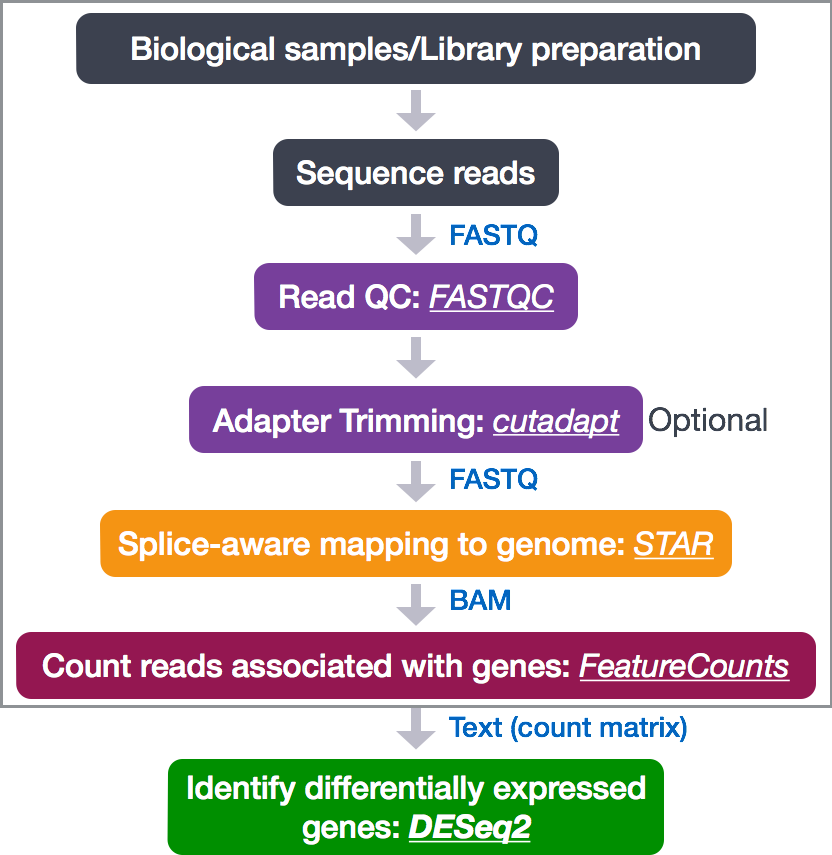
\includegraphics[width=4.16667in,height=\textheight,keepaspectratio]{img/rnaseq_full_workflow.png}

In the next few lessons, we will walk you through an \textbf{end-to-end gene-level RNA-seq differential expression workflow} using various R packages. We will start with the count matrix, perform exploratory data analysis for quality assessment and to explore the relationship between samples, perform differential expression analysis, and visually explore the results prior to performing downstream functional analysis.

\section{Review of the dataset}\label{review-of-the-dataset}

We will be using the full count matrix from the RNA-seq dataset that is part of a larger study described in \href{http://www.ncbi.nlm.nih.gov/pubmed/25464849}{Kenny PJ et al, Cell Rep 2014} investigating the interactions between genes potentially involved in Fragile X syndrome (FXS). FXS is a genetic disorder and the leading cause of inherited intellectual disabilities like autism. FXS is caused by aberrant production of a protein called Fragile X Messenger Ribonucleoprotein (\textbf{FMRP}) that is needed for brain development. People who have FXS do not make this protein. The authors demonstrated that \textbf{FMRP} associates with another RNA-binding protein \textbf{MOV10} (Mov10 RISC Complex RNA Helicase) and acts to regulate the translation of a subset of RNAs.

What is the function of \textbf{FMRP} and \textbf{MOV10}?

\begin{quote}
\textbf{FMRP} is ``most commonly found in the brain, is essential for normal cognitive development and female reproductive function. Mutations of this gene can lead to fragile X syndrome, mental retardation, premature ovarian failure, autism, Parkinson's disease, developmental delays and other cognitive deficits.'' - from \href{https://en.wikipedia.org/wiki/FMR1}{wikipedia}
\end{quote}

\begin{quote}
\textbf{MOV10} MOV10 has been shown to associate with the 3' UTR of mRNAs as part of its role in the RNA-induced silencing complex (RISC). MOV10 is an RNA helicase believed to assist in the unwinding of RNA duplexes. MOV10 is associated with \textbf{FMRP} in the context of the microRNA pathway. \textbf{MOV10} has a role in regulating translation: it facilitates microRNA-mediated translation of some RNAs, but it also increases expression of other RNAs.
\end{quote}

The aim of the RNAseq part of the study was to characterize the transcription expression patterns of \textbf{FMRP} and \textbf{MOV10} to identify overlapping target genes which would suggest that these genes are regulated by the \textbf{MOV10-FMRP} complex.

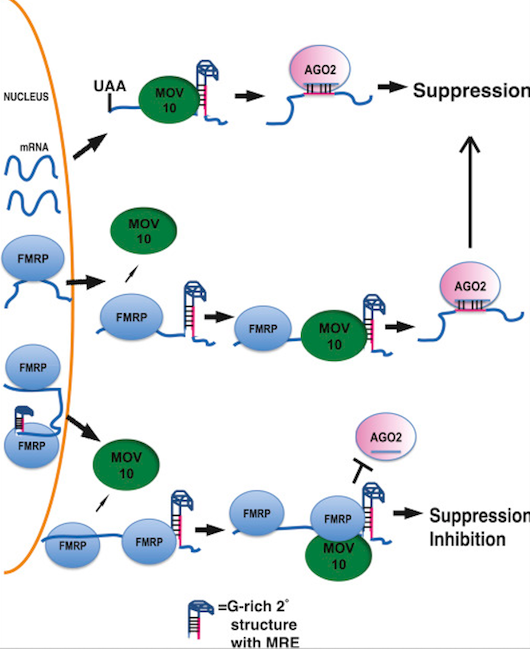
\includegraphics[width=4.16667in,height=\textheight,keepaspectratio]{img/model_mov10.png}

\textbf{Model for }MOV10-FMRP** Association in Translation Regulation\textbf{. Top: fate of RNAs bound by }MOV10\textbf{. }MOV10** binds the 3′ UTR-encoded G-rich structure to reveal MREs for subsequent AGO2 association. Middle: fate of RNAs bound by \textbf{FMRP}. \textbf{FMRP} binds RNAs in the nucleus. Upon export, \textbf{FMRP} recruits \textbf{MOV10}, which ultimately unwinds MREs for association with AGO2. Bottom: \textbf{FMRP} recruits \textbf{MOV10} to RNAs; however, binding of both \textbf{FMRP} and \textbf{MOV10} in proximity of MRE blocks association with AGO2. Red line indicates MRE.

RNA-seq was performed on HEK293F cells that were either transfected with a \textbf{MOV10} transgene, or siRNA to knock down Mov10 expression, or non-specific (irrelevant) siRNA. This resulted in 3 conditions \textbf{Mov10 oe} (over expression), \textbf{Mov10 kd} (knock down) and \textbf{Irrelevant kd}, respectively. The number of replicates is as shown below.

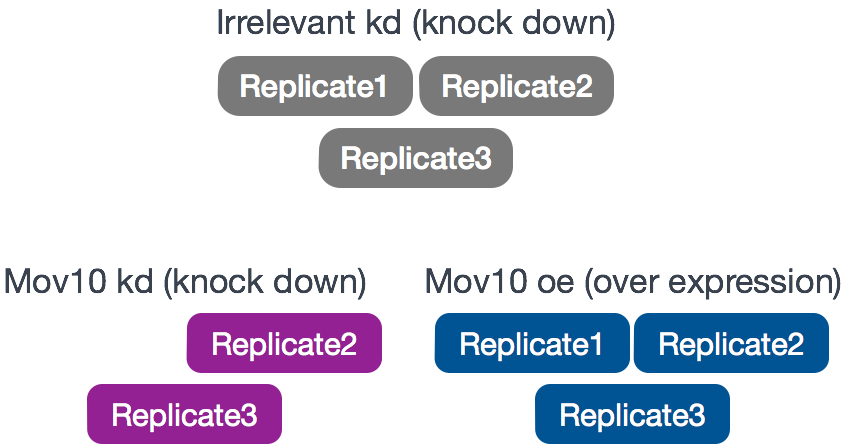
\includegraphics[width=4.16667in,height=\textheight,keepaspectratio]{img/dataset.png}

Using these data, we will evaluate transcriptional patterns associated with perturbation of \textbf{MOV10} expression. Please note that the irrelevant siRNA will be treated as our control condition.

\textbf{Links to raw data}
{[}GEO{]}: \url{https://www.ncbi.nlm.nih.gov/geo/query/acc.cgi?acc=GSE51443} ``Gene Expression Omnibus''
{[}SRA{]}: \url{https://trace.ncbi.nlm.nih.gov/Traces/sra/?study=SRP031507} ``Sequence Read Archive''

\textbf{Our questions:}

\begin{itemize}
\item
  What patterns of expression can we identify with the loss or gain of MOV10?
\item
  Are there any genes that are differentially expressed between the two conditions?
\item
  Are there any genes shared between the two conditions?
\end{itemize}

\section{Setting up}\label{setting-up}

Go to the \passthrough{\lstinline!File!} menu and to the \passthrough{\lstinline!lessons!} directory and open \passthrough{\lstinline!09-DGE\_codebook.Rmd!}. This will open in the script editor in the top left hand corner. This is where we will be running all commands required for this analysis, and like last time this is where you will enter the code/answers for your homework assignment. Please save this as something with your name in it (e.g.~\passthrough{\lstinline!firstname\_lastname\_09-DGE\_codebook.Rmd!}).

\pandocbounded{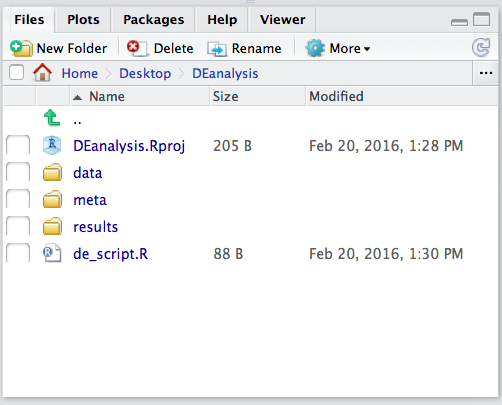
\includegraphics[keepaspectratio]{img/settingup.png}}

\subsection{Loading libraries}\label{loading-libraries}

For this analysis we will be using several R packages, some which have been installed from CRAN and others from Bioconductor. To use these packages (and the functions contained within them), we need to \textbf{load the libraries}.

\begin{lstlisting}[language=R]
## Setup Bioconductor and CRAN libraries used
library(tidyverse)
library(RColorBrewer)
library(DESeq2)
library(pheatmap)
library(ggplot2)
library(ggrepel)
\end{lstlisting}

\subsection{Loading data}\label{loading-data}

To load the data into our current environment, we will be using the \passthrough{\lstinline!read.table!} function. We need to provide the path to each file and also specify arguments to let R know that we have a header (\passthrough{\lstinline!header = T!}) and the first column is our row names (\passthrough{\lstinline!row.names = 1!}). By default the function expects tab-delimited files, which is what we have.

\begin{lstlisting}[language=R]
## Load in data
data <- read.table("data/Mov10_full_counts.txt", header = T, row.names = 1)

meta <- read.table("data/Mov10_full_meta.txt", header = T, row.names = 1)
\end{lstlisting}

Use \passthrough{\lstinline!class()!} to inspect our data and make sure we are working with data frames:

\begin{lstlisting}[language=R]
### Check classes of the data we just brought in
class(meta)
\end{lstlisting}

\section{{[}1{]} ``data.frame''}\label{data.frame}

\begin{lstlisting}[language=R]
class(data)
\end{lstlisting}

\section{{[}1{]} ``data.frame''}\label{data.frame-1}

\subsection{Viewing data}\label{viewing-data}

Make sure your datasets contain the expected samples / information before proceeding to perfom any type of analysis.

\begin{lstlisting}[language=R]
rownames(meta)
\end{lstlisting}

\section{{[}1{]} ``Irrel\_kd\_1'' ``Irrel\_kd\_2'' ``Irrel\_kd\_3'' ``Mov10\_kd\_2'' ``Mov10\_kd\_3''}\label{irrel_kd_1-irrel_kd_2-irrel_kd_3-mov10_kd_2-mov10_kd_3}

\section{{[}6{]} ``Mov10\_oe\_1'' ``Mov10\_oe\_2'' ``Mov10\_oe\_3''}\label{mov10_oe_1-mov10_oe_2-mov10_oe_3}

\begin{lstlisting}[language=R]
names(data)
\end{lstlisting}

\section{{[}1{]} ``Mov10\_kd\_2'' ``Mov10\_kd\_3'' ``Mov10\_oe\_1'' ``Mov10\_oe\_2'' ``Mov10\_oe\_3''}\label{mov10_kd_2-mov10_kd_3-mov10_oe_1-mov10_oe_2-mov10_oe_3}

\section{{[}6{]} ``Irrel\_kd\_1'' ``Irrel\_kd\_2'' ``Irrel\_kd\_3''}\label{irrel_kd_1-irrel_kd_2-irrel_kd_3}

You'll notice the colnames of the data are the sample names, and the rownames of the metadata are the sample names. This is important as we will be merging the metadata with the data based on the sample names.

\section{Differential gene expression analysis overview}\label{differential-gene-expression-analysis-overview}

So what does this count data actually represent? The count data used for differential expression analysis represents the number of sequence reads that originated from a particular gene. The higher the number of counts, the more reads associated with that gene, and the assumption that there was a higher level of expression of that gene in the sample.

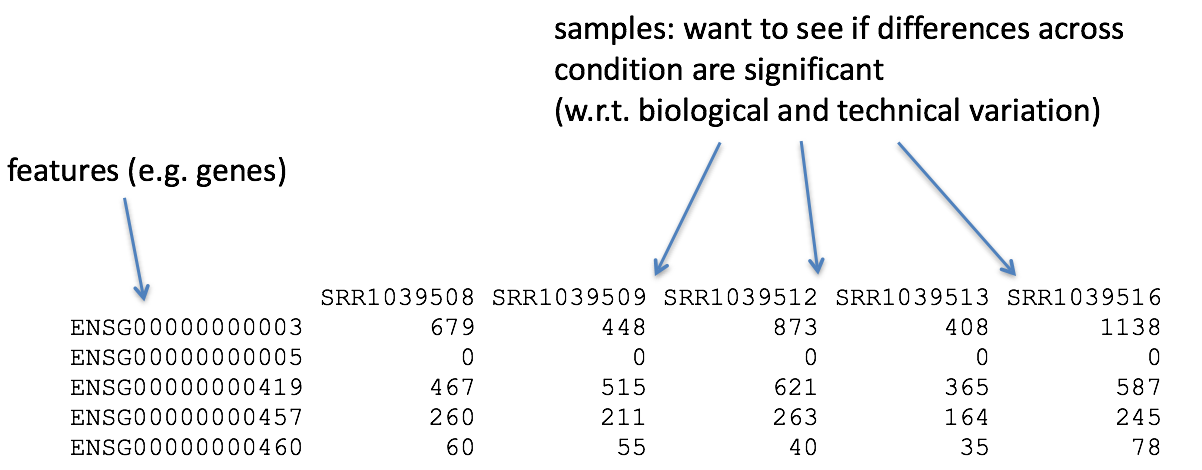
\includegraphics[width=6.25in,height=\textheight,keepaspectratio]{img/deseq_counts_overview.png}

With differential expression analysis, we are looking for genes that change in expression between two or more groups (defined in the metadata)
- case vs.~control
- correlation of expression with some variable or clinical outcome

\textbf{Why does it not work to identify differentially expressed gene by ranking the genes by how different they are between the two groups (based on fold change values)?}

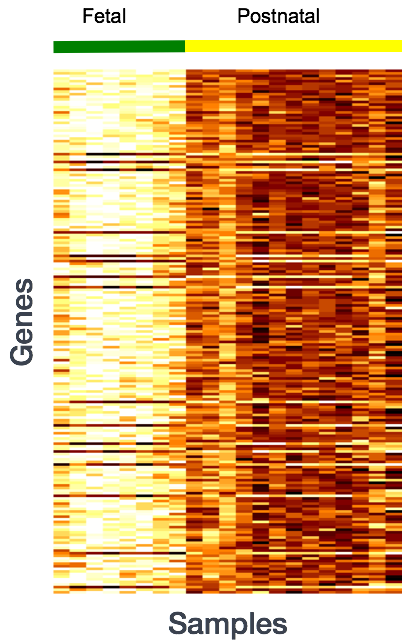
\includegraphics[width=2.08333in,height=\textheight,keepaspectratio]{img/foldchange_heatmap.png}

More often than not, there is much more going on with your data than what you are anticipating. Genes that vary in expression level between samples is a consequence of not only the experimental variables of interest but also due to extraneous sources. The goal of differential expression analysis to determine the relative role of these effects, and to separate the ``interesting'' from the ``uninteresting''.

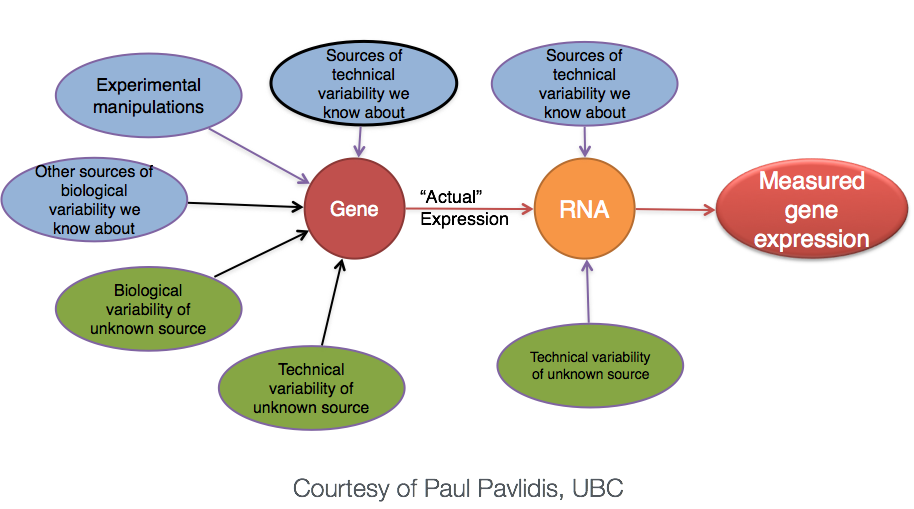
\includegraphics[width=5.20833in,height=\textheight,keepaspectratio]{img/de_variation.png}

The ``uninteresting'' presents as sources of variation in your data, and so even though the mean expression levels between sample groups may appear to be quite different, it is possible that the difference is not actually significant. This is illustrated for `GeneA' expression between `untreated' and `treated' groups in the figure below. The mean expression level of geneA for the `treated' group is twice as large as for the `untreated' group, but the variation between replicates indicates that this may not be a significant difference. \textbf{We need to take into account the variation in the data (and where it might be coming from) when determining whether genes are differentially expressed.}

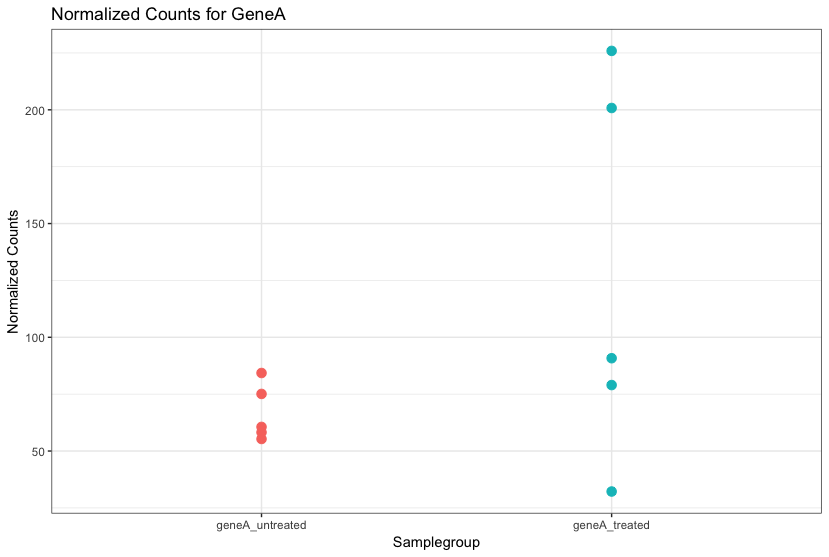
\includegraphics[width=4.16667in,height=\textheight,keepaspectratio]{img/de_norm_counts_var.png}

The goal of differential expression analysis is to determine, for each gene, whether the differences in expression (counts) \textbf{between groups} is significant given the amount of variation observed \textbf{within groups} (replicates). To test for significance, we need an appropriate statistical model that accurately performs normalization (to account for differences in sequencing depth, etc.) and variance modeling (to account for few numbers of replicates and large dynamic expression range).

\subsection{RNA-seq count distribution}\label{rna-seq-count-distribution}

To determine the appropriate statistical model, we need information about the distribution of counts. To get an idea about how RNA-seq counts are distributed, let's plot the counts for a single sample, `Mov10\_oe\_1':

\begin{lstlisting}[language=R]
ggplot(data) + geom_histogram(aes(x = Mov10_oe_1), stat = "bin", bins = 200) + xlab("Raw expression counts") +
    ylab("Number of genes")
\end{lstlisting}

\pandocbounded{\includegraphics[keepaspectratio]{2025_RNA-Seq-Analysis_files/figure-latex/unnamed-chunk-6-1.pdf}}

If we zoom in close to zero, we can see a large number of genes with counts of zero:

\begin{lstlisting}[language=R]
ggplot(data) + geom_histogram(aes(x = Mov10_oe_1), stat = "bin", bins = 200) + xlim(-5,
    500) + xlab("Raw expression counts") + ylab("Number of genes")
\end{lstlisting}

\pandocbounded{\includegraphics[keepaspectratio]{2025_RNA-Seq-Analysis_files/figure-latex/unnamed-chunk-7-1.pdf}}

These images illustrate some common features of RNA-seq count data, including a \textbf{low number of counts associated with a large proportion of genes}, and a long right tail due to the \textbf{lack of any upper limit for expression}.

\subsection{Modeling count data}\label{modeling-count-data}

Count data is often modeled using the \textbf{binomial distribution}. The Binomial distribution is a common probability distribution that models the probability of obtaining one of two outcomes under a given number of parameters. It summarizes the number of successes in a fixed number of trials when each trial has two possible outcomes. For example, a coin toss is typically modeled using a binomial distribution, where the number of successes (e.g., heads) in a fixed number of trials (e.g., 10 coin tosses) when each trial has two possible outcomes (e.g., heads or tails) and the probability of success is constant. However, not all count data can be fit with the binomial distribution. The binomial is based on discrete events and used in situations when you have a certain number of cases.

The \textbf{binomial distribution} is used to model scenarios where there are two possible outcomes, such as ``success'' or ``failure,'' over a fixed number of trials. For example, flipping a coin 10 times and counting the number of ``heads'' out of those 10 flips follows a binomial distribution with a probability of success (\(p\)) equal to 0.5.

When \textbf{the number of cases is very large (i.e.~people who buy lottery tickets), but the probability of an event is very small (probability of winning)}, the \textbf{Poisson distribution} is used to model these types of count data.

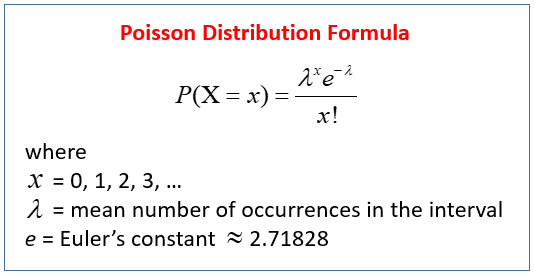
\includegraphics[width=3.125in,height=\textheight,keepaspectratio]{img/poisson-distribution-formula.png}

\textbf{With RNA-seq data, for each sample we have millions of reads being sequenced and the probability of a read mapping to a gene is extremely low.} Thus, it would be an appropriate situation to use the Poisson distribution. However, a unique property of this distribution is that the mean == variance given by the single parameter \(\lambda\).

For us to apply a poisson distribution to our data, we first need to find out
whether our data fulfills the criteria to use the poisson distribution. To do that we can plot the \emph{mean versus variance} for the `Mov10 overexpression' replicates:

To calculate the mean and variance of our data, we will use the \passthrough{\lstinline!apply!} function. The \passthrough{\lstinline!apply!} function allows you to apply a function to the margins (rows or columns) of a matrix. The syntax for \passthrough{\lstinline!apply!} is as follows: \passthrough{\lstinline!apply(X, MARGIN, FUN)!}, where \passthrough{\lstinline!X!} is a matrix, \passthrough{\lstinline!MARGIN!} is the margin of the matrix to apply the function to (1 = rows, 2 = columns), and \passthrough{\lstinline!FUN!} is the function to apply.

We will use \passthrough{\lstinline!MARGIN = 1!} to apply the function mean and variance of the counts for each row (gene) across the `Mov10 overexpression' replicates. We will then create a data frame with the mean and variance of the counts for each gene.

\begin{lstlisting}[language=R]
# calculate the mean and variance of the counts for each gene
mean_counts <- apply(data[, 3:5], 1, mean)

variance_counts <- apply(data[, 3:5], 1, var)

# for ggplot we need the data to be in a data.frame
df <- data.frame(mean_counts, variance_counts)
\end{lstlisting}

Run the following code to plot the \emph{mean versus variance} for the `Mov10 overexpression' replicates:

\begin{lstlisting}[language=R]
ggplot(df) + geom_point(aes(x = mean_counts, y = variance_counts)) + geom_line(aes(x = mean_counts,
    y = mean_counts, color = "red")) + scale_y_log10() + scale_x_log10()
\end{lstlisting}

\pandocbounded{\includegraphics[keepaspectratio]{2025_RNA-Seq-Analysis_files/figure-latex/unnamed-chunk-9-1.pdf}}

By plotting the \emph{mean versus the variance} of our data we can easily see that the \textbf{variance \textgreater{} mean} and therefore it does not fit the Poisson distribution. Genes having higher mean counts have even higher variance. Also for gene having low mean counts, there is a scatter of points and we can see that there is variability even in the variance. To account for this extra variance we need a new model.

The model that fits best, given this type of variability between replicates, is the \textbf{Negative Binomial (NB) model}. Essentially, \textbf{the NB model} is a good approximation for data where the \textbf{variance \textgreater{} mean}, as is the case with RNA-seq count data.

\subsection{Improving mean estimates (i.e.~reducing variance) with biological replicates}\label{improving-mean-estimates-i.e.-reducing-variance-with-biological-replicates}

The variance or scatter tends to reduce as we increase the number of biological replicates (\emph{the distribution will approach the Poisson distribution with increasing numbers of replicates}). \textbf{The value of additional replicates is that as you add more data (replicates), you get increasingly precise estimates of group means, and ultimately greater confidence in the ability to distinguish differences between sample classes (i.e.~more DE genes).}

The figure below shows how the number of differentially expressed (DE) genes identified is influenced by sequencing depth and number of replicates {[}\href{https://academic.oup.com/bioinformatics/article/30/3/301/228651/RNA-seq-differential-expression-studies-more}{1}{]}. Notice that increasing the number of replicates identifies more DE genes compared to increasing sequencing depth. This is because most of the biological variability occurs between samples. As a result, having more replicates typically yields better results than increasing sequencing depth, as it captures natural biological variability more effectively and leads to more accurate estimates of within-group variation. While increasing sequencing depth reduces technical noise, it has less impact on detecting DE genes since it doesn't account for biological variability. Generally, a minimum sequencing depth of 20-30 million reads per sample is recommended, though successful RNA-seq experiments have been conducted with as few as 10 million reads when enough replicates are included.

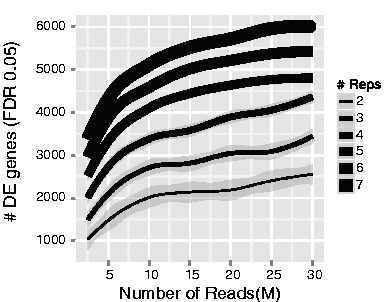
\includegraphics[width=5.20833in,height=\textheight,keepaspectratio]{img/de_replicates_img.png}

\begin{quote}
\textbf{NOTE}

\begin{itemize}
\tightlist
\item
  \textbf{Biological replicates} represent multiple samples (i.e.~RNA from different mice) representing the same sample class
\item
  \textbf{Technical replicates} represent the same sample (i.e.~RNA from the same mouse) but with technical steps replicated
\item
  Usually biological variance is much greater than technical variance, so we do not need to account for technical variance to identify biological differences in expression
\item
  \textbf{Don't spend money on technical replicates - biological replicates are much more useful}
\end{itemize}
\end{quote}

\subsection{Differential expression analysis workflow}\label{differential-expression-analysis-workflow}

To model counts appropriately when performing a differential expression analysis, there are a number of software packages that have been developed for differential expression analysis of RNA-seq data. Even as new methods are continuously being developed a few tools are generally recommended as best practice, e.g.~\textbf{\href{https://bioconductor.org/packages/release/bioc/html/DESeq2.html}{DESeq2}} and \textbf{\href{https://bioconductor.org/packages/release/bioc/html/edgeR.html}{EdgeR}}. Both these tools use the negative binomial model, employ similar methods, and typically, yield similar results. They are pretty stringent, and have a good balance between sensitivity and specificity (reducing both false positives and false negatives).

Here is a comparison of the three most highy used software packages for differential expression analysis. No single method is optimal under all circumstances, for example, limma works best when sample number is high, and edgeR and DESeq2 perform well for small sample sizes. It is also difficult to compare analysis methods due to different procedures in calculating pvalues.

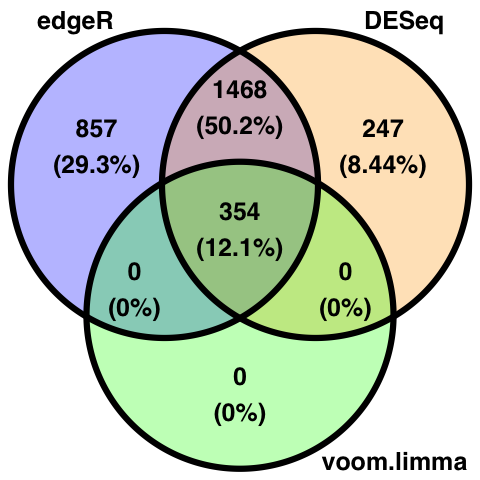
\includegraphics[width=3.125in,height=\textheight,keepaspectratio]{img/venn.png}

\textbf{We will be using \href{https://genomebiology.biomedcentral.com/articles/10.1186/s13059-014-0550-8}{DESeq2} for the DE analysis, and the analysis steps with DESeq2 are shown in the flowchart below}. DESeq2 first normalizes the count data to account for differences in library sizes and RNA composition between samples. Then, we will use the normalized counts to make some plots for QC at the gene and sample level. The final step is to use the appropriate functions from the DESeq2 package to perform the differential expression analysis.

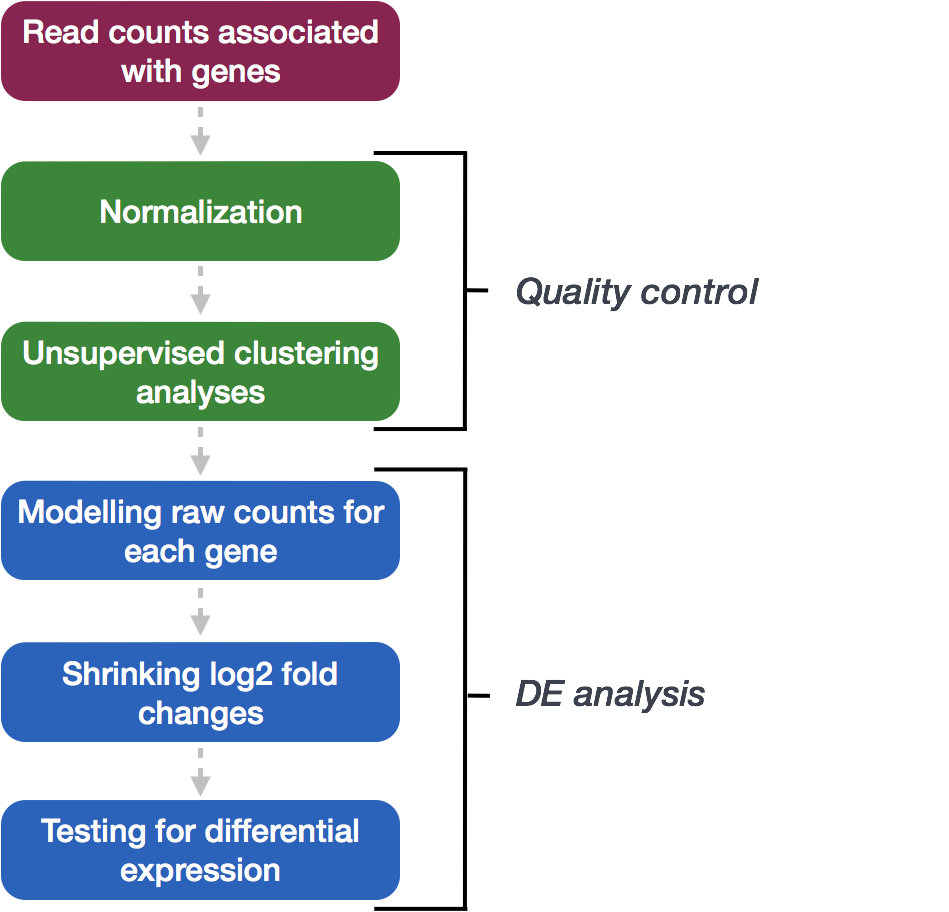
\includegraphics[width=5.20833in,height=\textheight,keepaspectratio]{img/deseq_workflow_full_2018.png}

We will go in-depth into each of these steps in the following lessons, but additional details and helpful suggestions regarding DESeq2 can be found in the \href{http://bioconductor.org/packages/devel/bioc/vignettes/DESeq2/inst/doc/DESeq2.html}{DESeq2 vignette}. As you go through this workflow and questions arise, you can reference the vignette from within RStudio:

\begin{lstlisting}[language=R]
vignette("DESeq2")
\end{lstlisting}

This is very convenient, as it provides a wealth of information at your fingertips! Be sure to use this as you need during the workshop.

\begin{center}\rule{0.5\linewidth}{0.5pt}\end{center}

\chapter{Count normalization}\label{count-normalization}

\section{Normalization}\label{normalization}

The first step in the DE analysis workflow is count normalization, which is necessary to make accurate comparisons of gene expression between samples.

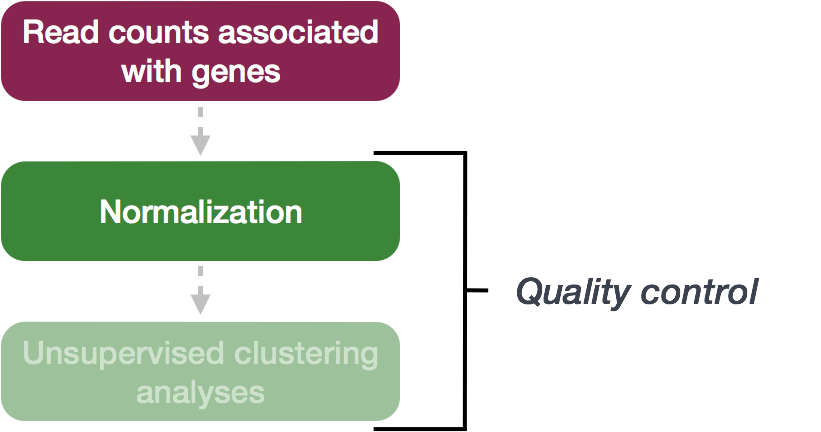
\includegraphics[width=4.16667in,height=\textheight,keepaspectratio]{img/deseq_workflow_normalization_2018.png}

The counts of mapped reads for each gene is proportional to the expression of RNA (``interesting'') in addition to many other factors (``uninteresting''). Normalization is the process of scaling raw count values to account for the ``uninteresting'' factors. In this way the expression levels are more comparable between and/or within samples.

The main factors often considered during normalization are:

\begin{itemize}
\tightlist
\item
  \textbf{Sequencing depth:}
\end{itemize}

Accounting for sequencing depth is necessary for comparison of gene expression between samples. In the example below, each gene appears to have doubled in expression in \emph{Sample A} relative to \emph{Sample B}, however this is a consequence of \emph{Sample A} having double the sequencing depth.

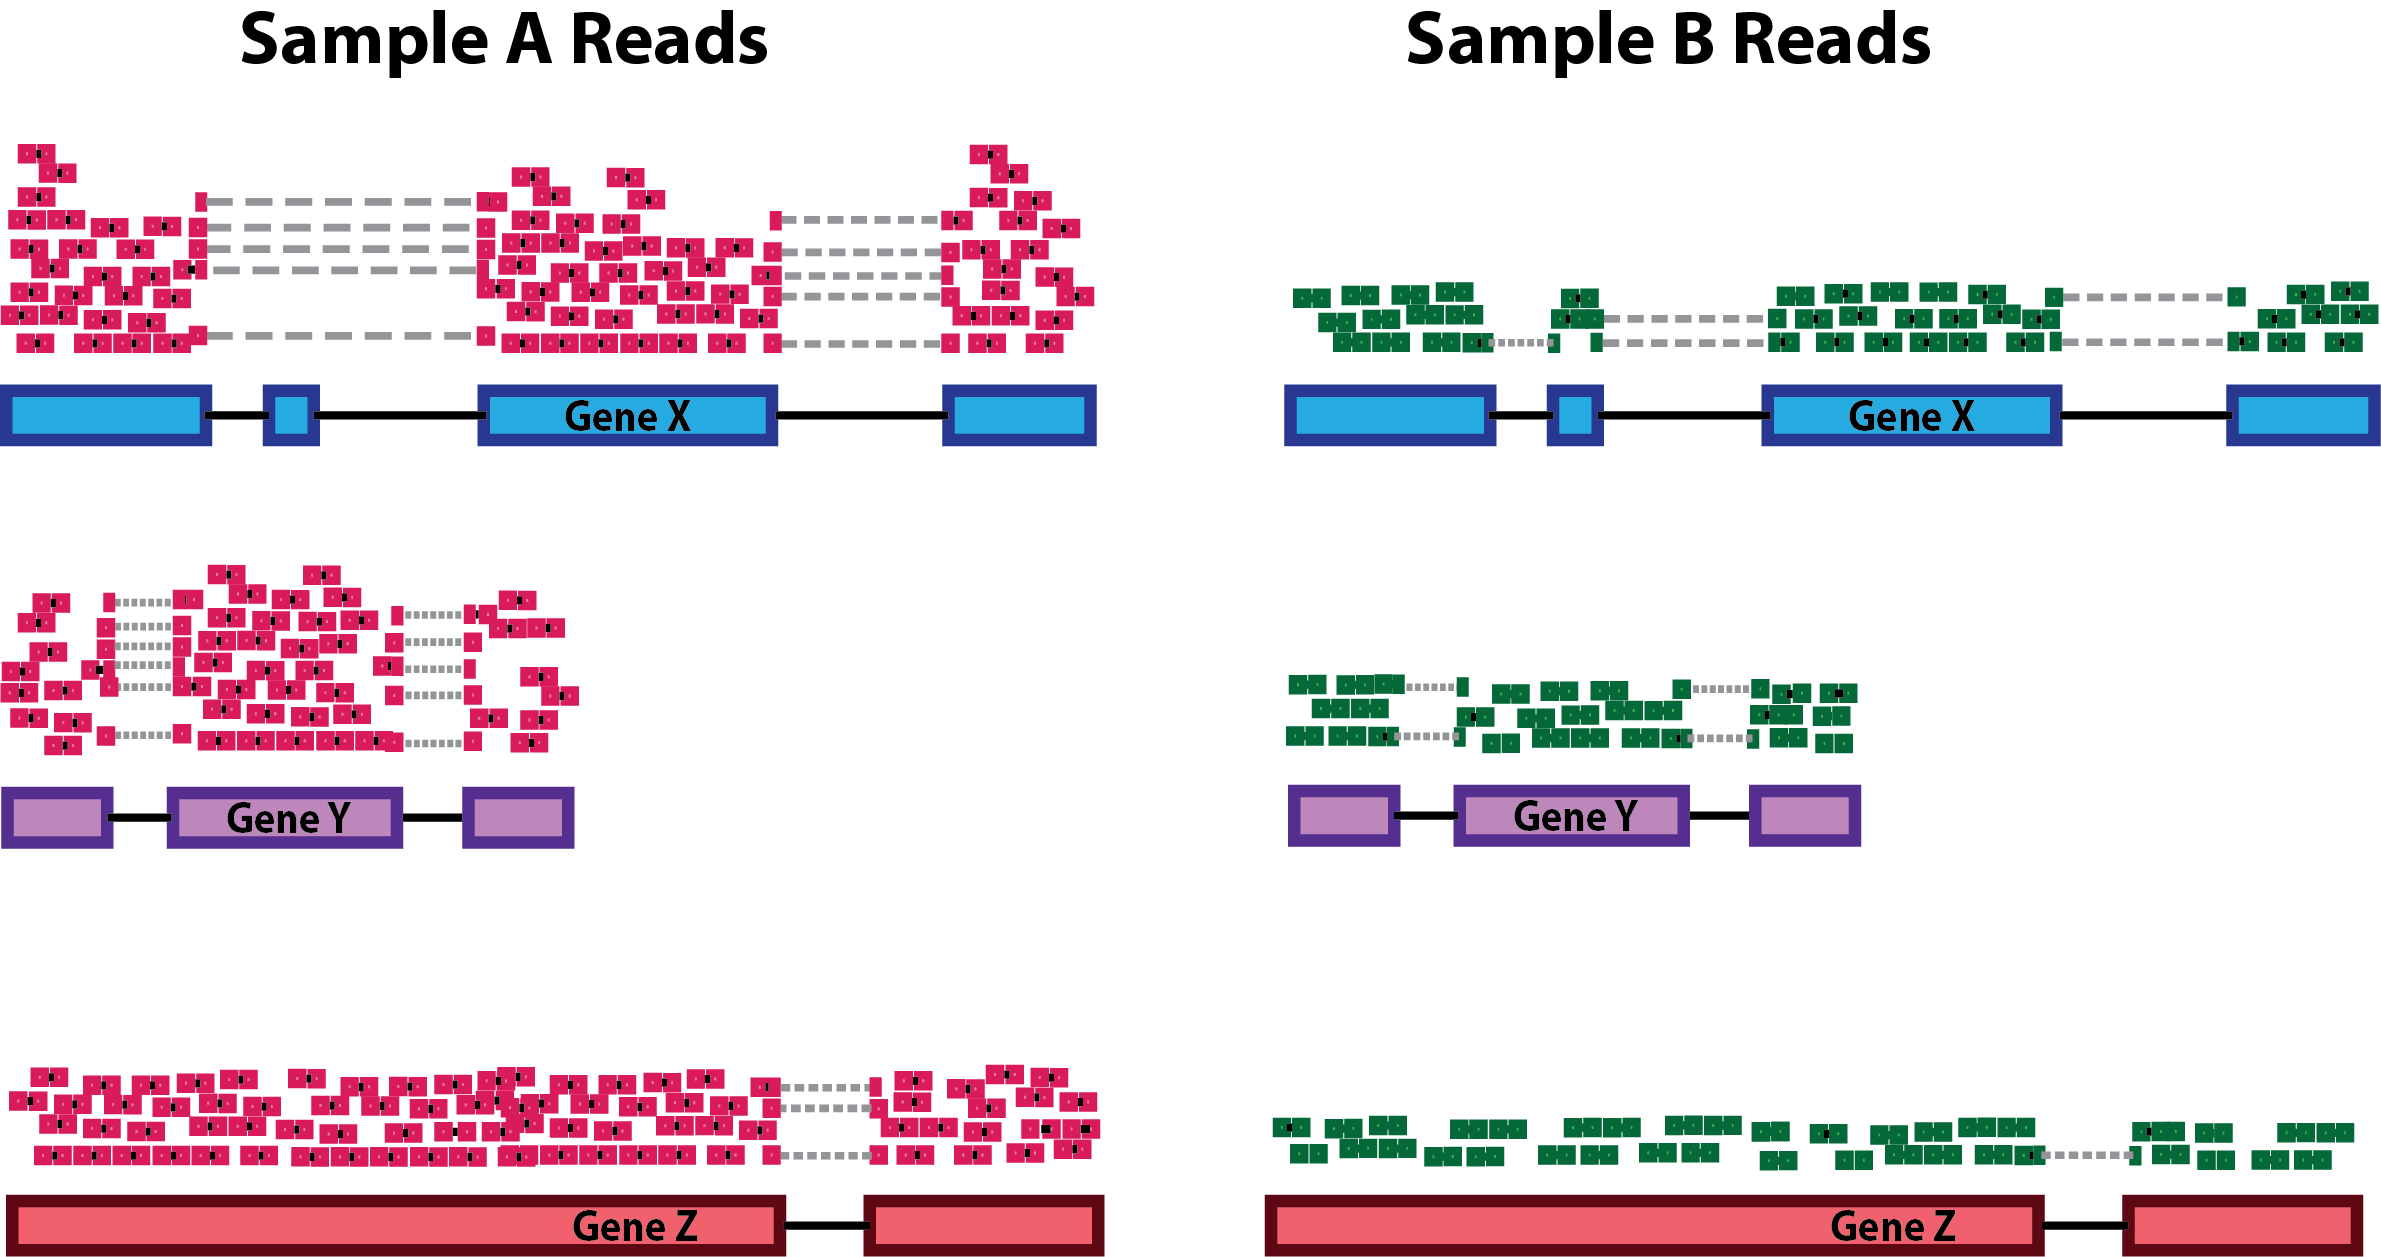
\includegraphics[width=4.16667in,height=\textheight,keepaspectratio]{img/normalization_methods_depth.png}

\begin{quote}
\emph{\textbf{NOTE:} In the figure above, each pink and green rectangle represents a read aligned to a gene. Reads connected by dashed lines connect a read spanning an intron.}
\end{quote}

\begin{itemize}
\tightlist
\item
  \textbf{Gene length:}
\end{itemize}

Accounting for gene length is necessary for comparing expression between different genes within the same sample. In the example, \emph{Gene X} and \emph{Gene Y} have similar levels of expression, but the number of reads mapped to \emph{Gene X} would be many more than the number mapped to \emph{Gene Y} because \emph{Gene X} is longer.

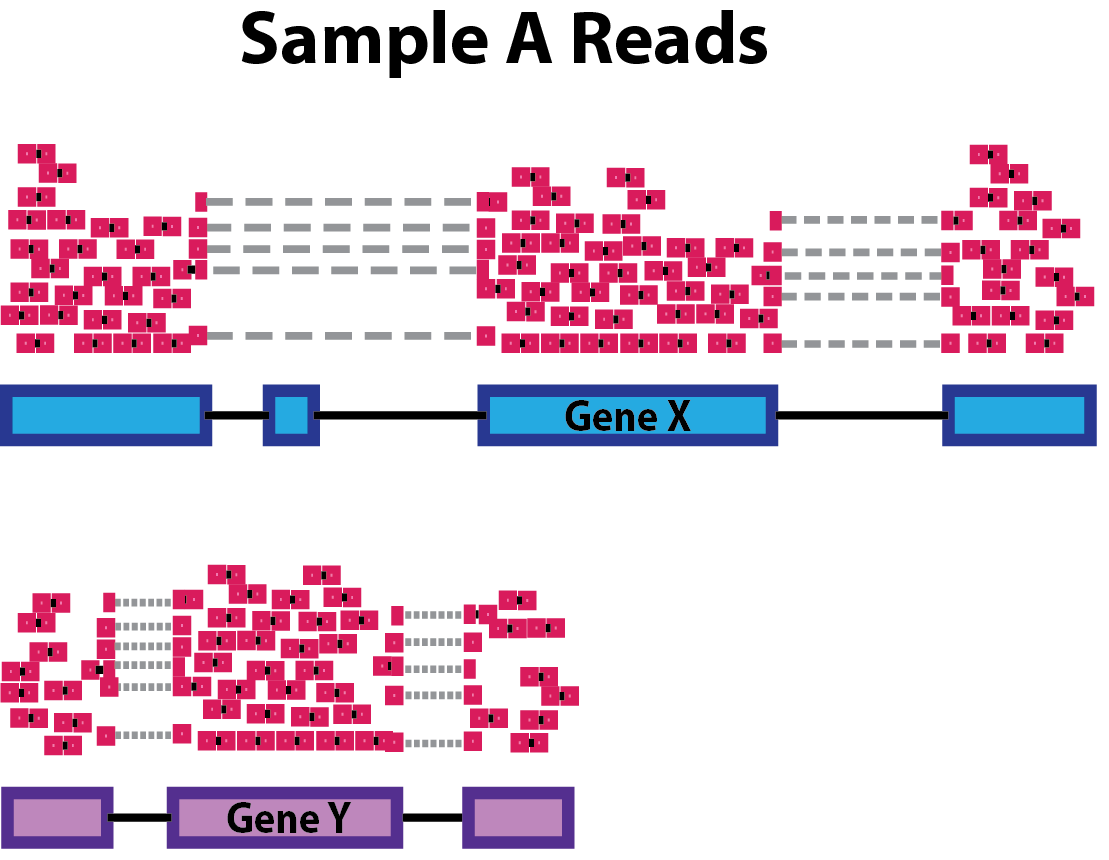
\includegraphics[width=2.08333in,height=\textheight,keepaspectratio]{img/normalization_methods_length.png}

\begin{itemize}
\tightlist
\item
  \textbf{RNA composition:}
\end{itemize}

RNA composition bias arises when a few highly expressed genes dominate the overall expression profile of a sample. Accounting for RNA composition is recommended for accurate comparison of expression between samples, and is particularly important when performing differential expression analyses {[}\href{https://genomebiology.biomedcentral.com/articles/10.1186/gb-2010-11-10-r106}{1}{]}.

In the example, if we were to divide each sample by the total number of counts to normalize, the counts would be greatly skewed by the DE gene, which takes up most of the counts for \emph{Sample A}, but not \emph{Sample B}. Most other genes for \emph{Sample A} would be divided by the larger number of total counts and appear to be less expressed than those same genes in \emph{Sample B}.

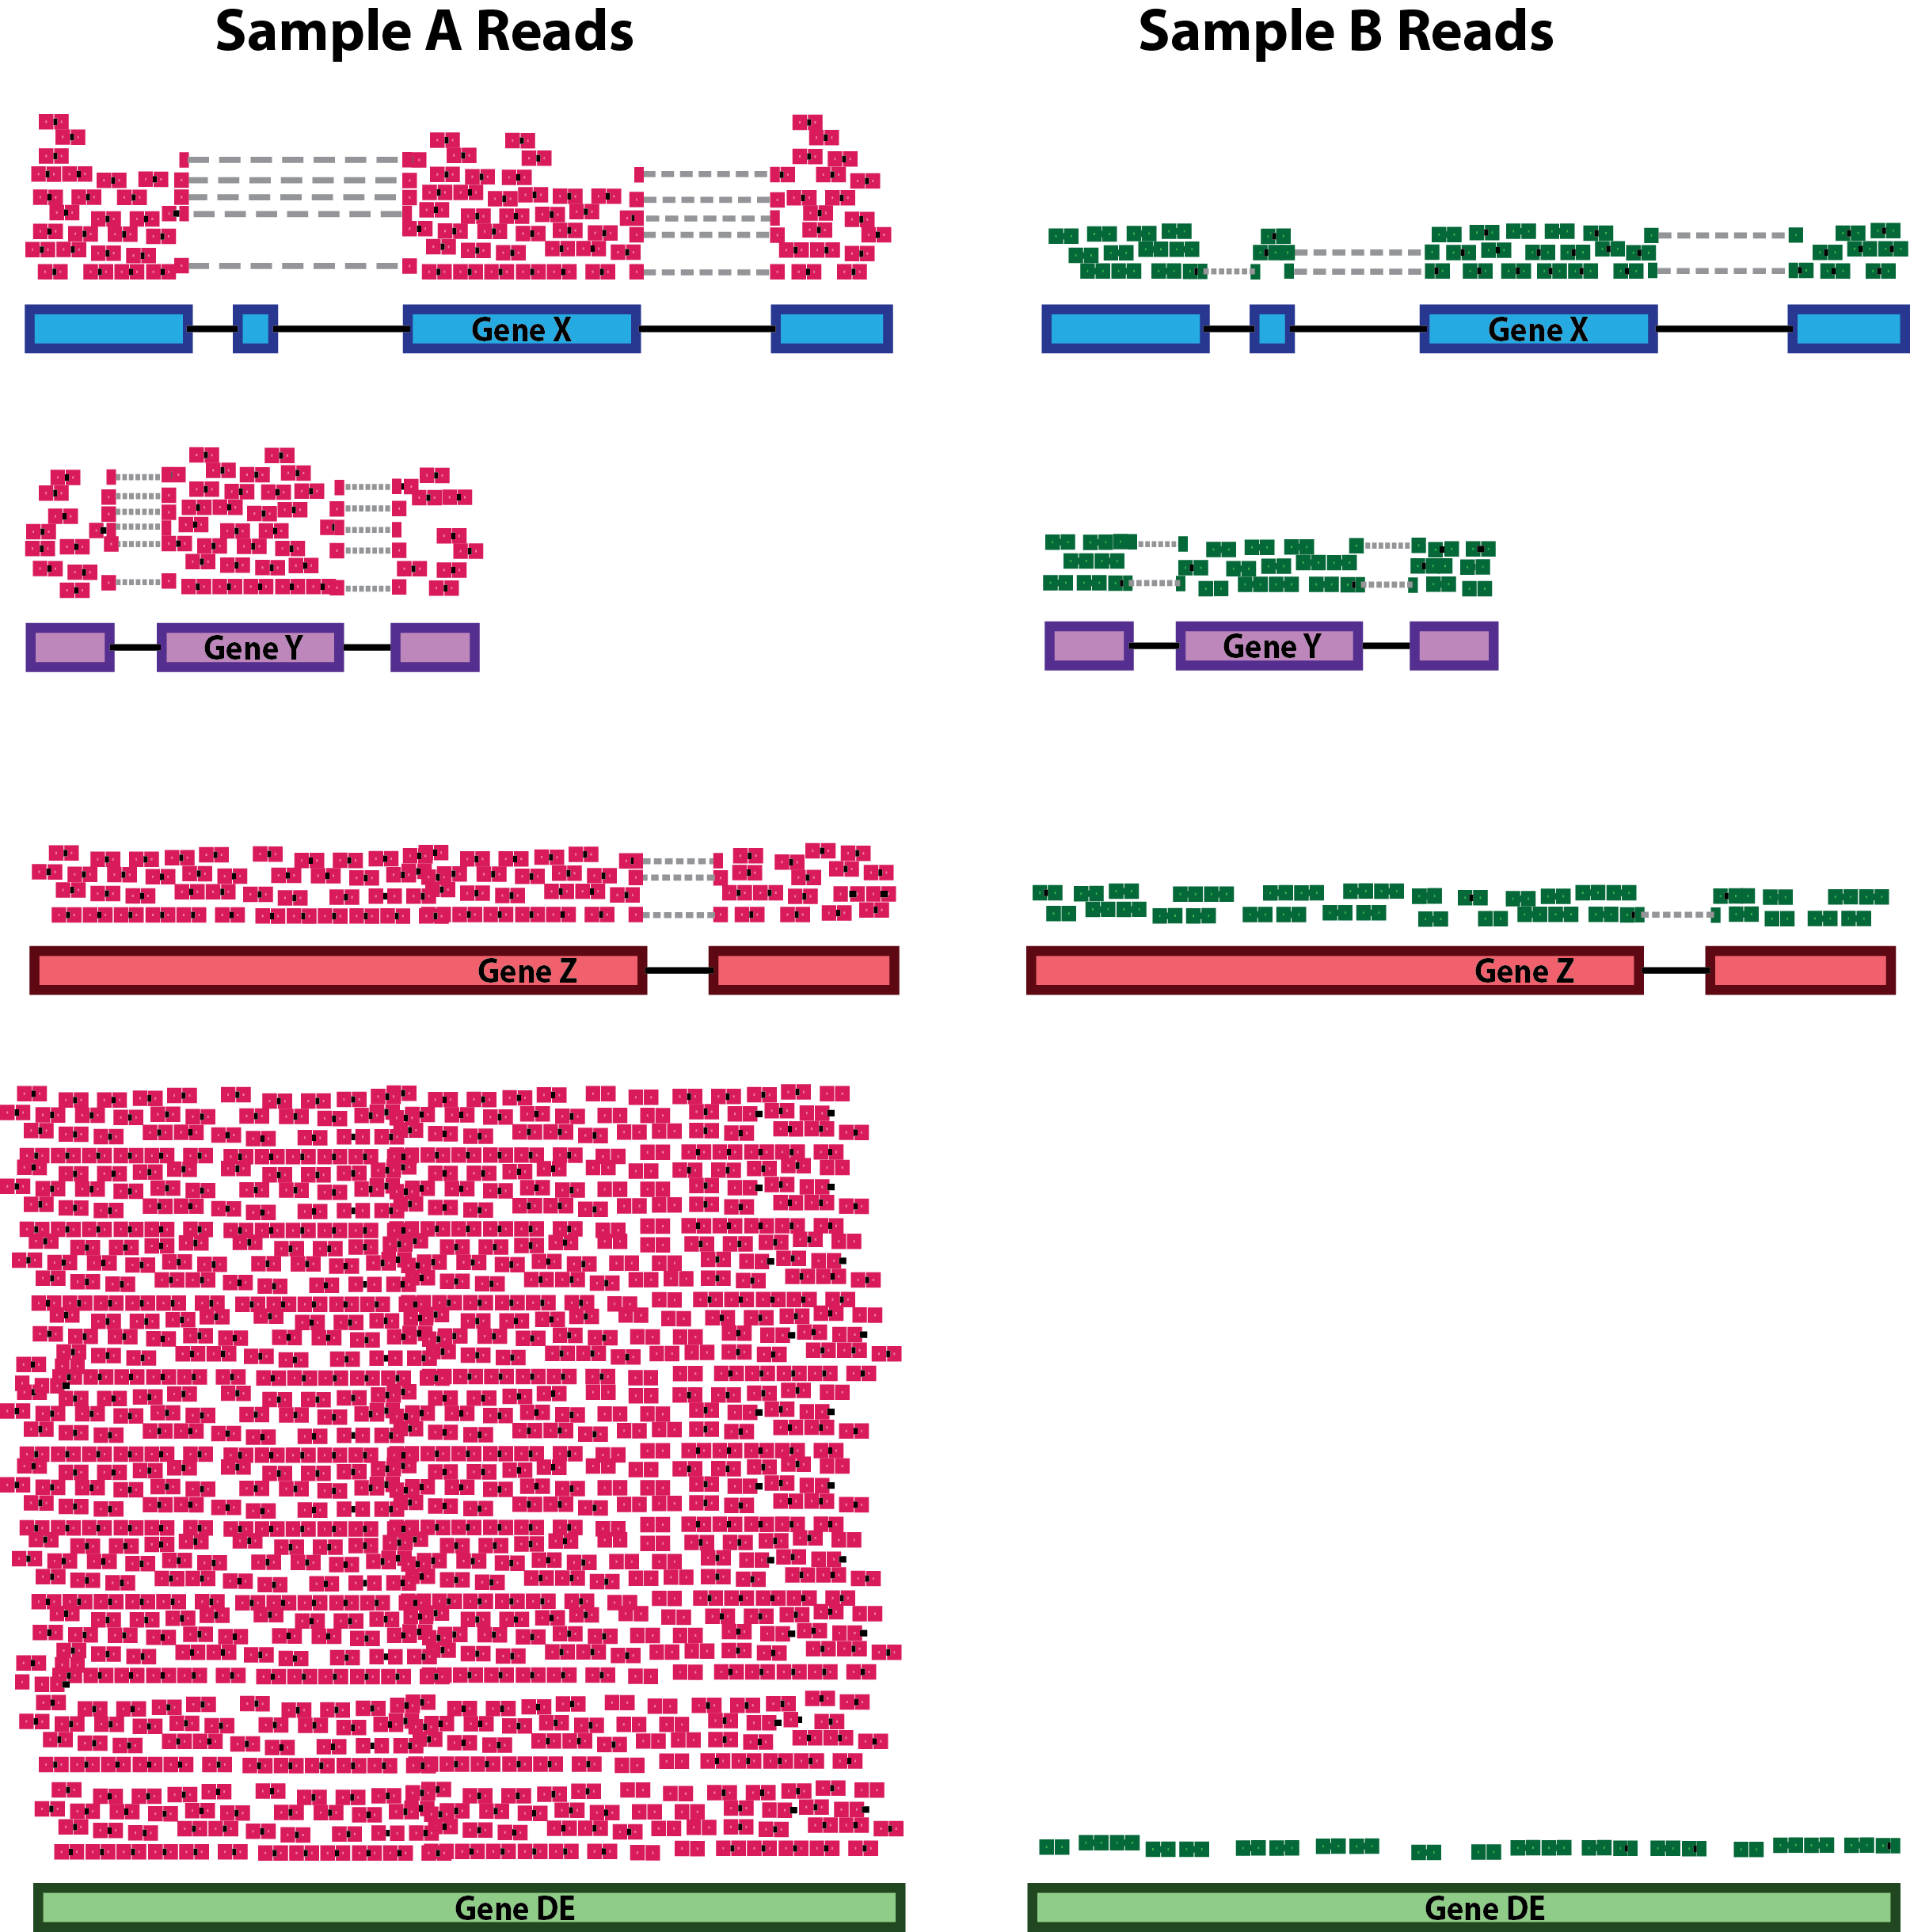
\includegraphics[width=4.16667in,height=\textheight,keepaspectratio]{img/normalization_methods_composition.png}

\textbf{\emph{While normalization is essential for differential expression analyses, it is also necessary for exploratory data analysis, visualization of data, and whenever you are exploring or comparing counts between or within samples.}}

\subsection{Common normalization methods}\label{common-normalization-methods}

Several common normalization methods exist to account for these differences:

TPM is very similar to RPKM and FPKM. The only difference is the order of operations. Here's how you calculate TPM:

For example, here's how you would calculate TPM for a gene in a sample:

\begin{enumerate}
\def\labelenumi{\arabic{enumi}.}
\tightlist
\item
  Divide the read counts by the length of each gene in kilobases. This gives you reads per kilobase (RPK).
\end{enumerate}

\[
RPK = \frac{reads}{gene length (kb)}
\]

\begin{enumerate}
\def\labelenumi{\arabic{enumi}.}
\setcounter{enumi}{1}
\tightlist
\item
  Count up all the RPK values in a sample and divide this number by 1,000,000. This is your ``per million'' scaling factor.
\end{enumerate}

\[
\text{Per million scaling factor} = \frac{\sum RPK}{1,000,000}
\]

\begin{enumerate}
\def\labelenumi{\arabic{enumi}.}
\setcounter{enumi}{2}
\tightlist
\item
  Divide the RPK values by the ``per million'' scaling factor. This gives you TPM.
\end{enumerate}

\[
TPM = \frac{RPK}{\text{Per million scaling factor}}
\]

The key idea here is that \textbf{TPM} normalizes for both \textbf{gene length} and \textbf{sequencing depth}, making it easier to compare the \textbf{relative abundance} of genes across different samples, regardless of how many total reads were generated.

\begin{longtable}[]{@{}
  >{\raggedright\arraybackslash}p{(\linewidth - 6\tabcolsep) * \real{0.2500}}
  >{\raggedright\arraybackslash}p{(\linewidth - 6\tabcolsep) * \real{0.2500}}
  >{\raggedright\arraybackslash}p{(\linewidth - 6\tabcolsep) * \real{0.2500}}
  >{\raggedright\arraybackslash}p{(\linewidth - 6\tabcolsep) * \real{0.2500}}@{}}
\toprule\noalign{}
\begin{minipage}[b]{\linewidth}\raggedright
Normalization method
\end{minipage} & \begin{minipage}[b]{\linewidth}\raggedright
Description
\end{minipage} & \begin{minipage}[b]{\linewidth}\raggedright
Accounted factors
\end{minipage} & \begin{minipage}[b]{\linewidth}\raggedright
Recommendations for use
\end{minipage} \\
\midrule\noalign{}
\endhead
\bottomrule\noalign{}
\endlastfoot
\textbf{TPM} (transcripts per kilobase million) & counts per length of transcript (kb) per million reads mapped & sequencing depth and gene length & gene count comparisons within a sample or between samples of the same sample group; \textbf{NOT for DE analysis} \\
\textbf{RPKM/FPKM} (reads/fragments per kilobase of exon per million reads/fragments mapped) & similar to TPM & sequencing depth and gene length & gene count comparisons between genes within a sample; \textbf{NOT for between sample comparisons or DE analysis} \\
DESeq2's \textbf{median of ratios} {[}\href{https://genomebiology.biomedcentral.com/articles/10.1186/gb-2010-11-10-r106}{1}{]} & counts divided by sample-specific size factors determined by median ratio of gene counts relative to geometric mean per gene & sequencing depth and RNA composition & gene count comparisons between samples and for \textbf{DE analysis}; \textbf{NOT for within sample comparisons} \\
EdgeR's \textbf{trimmed mean of M values (TMM)} {[}\href{https://genomebiology.biomedcentral.com/articles/10.1186/gb-2010-11-3-r25}{2}{]} & uses a weighted trimmed mean of the log expression ratios between samples & sequencing depth, RNA composition & gene count comparisons between samples and for \textbf{DE analysis}; \textbf{NOT for within sample comparisons} \\
\end{longtable}

\subsection{TPM (Not Recommended)}\label{tpm-not-recommended}

\textbf{Step 1: Calculate Reads Per Kilobase (RPK)}

To calculate RPK for each gene in each sample, divide the read counts by the gene length in kilobases.

\begin{longtable}[]{@{}lccc@{}}
\toprule\noalign{}
Gene & Sample 1 (reads) & Sample 2 (reads & Length \\
\midrule\noalign{}
\endhead
\bottomrule\noalign{}
\endlastfoot
Gene A & 300 & 600 & 1 kb \\
Gene B & 500 & 400 & 2 kb \\
\end{longtable}

\textbf{Sample 1:}
- Gene A RPK = 300 reads / 1 kb = 300
- Gene B RPK = 500 reads / 2 kb = 250

\textbf{Sample 2:}
- Gene A RPK = 600 reads / 1 kb = 600
- Gene B RPK = 400 reads / 2 kb = 200

\begin{longtable}[]{@{}lcc@{}}
\toprule\noalign{}
Gene & Sample 1 (RPK) & Sample 2 (RPK) \\
\midrule\noalign{}
\endhead
\bottomrule\noalign{}
\endlastfoot
Gene A & 300 & 600 \\
Gene B & 250 & 200 \\
\end{longtable}

\textbf{Step 2: Calculate the Per-Million Scaling Factor}

Sum the RPK values in each sample and divide by 1,000,000.

\textbf{Sample 1:}
- Total RPK = 300 + 250 = 550
- Scaling Factor = 550 / 1,000,000 = 0.00055

\textbf{Sample 2:}
- Total RPK = 600 + 200 = 800
- Scaling Factor = 800 / 1,000,000 = 0.0008

\textbf{Step 3: Calculate TPM}

Now, divide each gene's RPK by the per-million scaling factor to get the TPM.

\textbf{Sample 1:}
- Gene A TPM = 300 / 0.00055 = 545,455
- Gene B TPM = 250 / 0.00055 = 454,545

\textbf{Sample 2:}
- Gene A TPM = 600 / 0.0008 = 750,000
- Gene B TPM = 200 / 0.0008 = 250,000

\begin{longtable}[]{@{}lcc@{}}
\toprule\noalign{}
Gene & Sample 1 (TPM) & Sample 2 (TPM) \\
\midrule\noalign{}
\endhead
\bottomrule\noalign{}
\endlastfoot
Gene A & 545,455 & 750,000 \\
Gene B & 454,545 & 250,000 \\
\end{longtable}

TPM normalizes read counts by the total reads in a sample, allowing comparisons between genes while accounting for gene length. However, it does not account for the variability inherent in count data or overdispersion, making statistical testing on these values unreliable.

\subsection{RPKM/FPKM (Not Recommended)}\label{rpkmfpkm-not-recommended}

Using RPKM/FPKM normalization means the total normalized counts will vary between samples, making direct comparisons between genes unreliable.

\begin{longtable}[]{@{}lcc@{}}
\toprule\noalign{}
Gene & Sample A & Sample B \\
\midrule\noalign{}
\endhead
\bottomrule\noalign{}
\endlastfoot
XCR1 & 5.5 & 5.5 \\
WASHC1 & 73.4 & 21.8 \\
\ldots{} & \ldots{} & \ldots{} \\
Total RPKM & 1,000,000 & 1,500,000 \\
\end{longtable}

For example, even though both samples show XCR1 as 5.5, they cannot be directly compared because their total counts differ.

\textbf{Conclusion:}
Tools like DESeq2 or edgeR are better suited for differential expression analysis, as they:

\begin{itemize}
\item
  Use raw counts for more accurate modeling.
\item
  Apply statistical modeling (e.g., Negative Binomial) to account for variance across replicates.
\end{itemize}

\subsection{DESeq2 Normalization: Median of Ratios Method}\label{deseq2-normalization-median-of-ratios-method}

For differential expression analysis, gene length need not be factored in; however, \textbf{sequencing depth} and \textbf{RNA composition} must be considered. The median of ratios method neutralizes these differences.

This method involves several steps, even though from the user-end it appears as a single function call in DESeq2.

\textbf{Step 1: Create a Pseudo-reference Sample (Row-wise Geometric Mean)}

The \textbf{geometric mean} of a set of \(n\) positive numbers \(x_1, x_2, \dots, x_n\) is defined as:

\[
\text{Geometric Mean} = \left( \prod_{i=1}^{n} x_i \right)^{\frac{1}{n}}
\]

For each gene, a pseudo-reference sample is created that is equal to the geometric mean across all samples, reducing the impact of extreme values.

\begin{longtable}[]{@{}lccc@{}}
\toprule\noalign{}
Gene & Sample A & Sample B & Pseudo-reference Sample \\
\midrule\noalign{}
\endhead
\bottomrule\noalign{}
\endlastfoot
EF2A & 1489 & 906 & sqrt(1489 * 906) = \textbf{1161.5} \\
ABCD1 & 22 & 13 & sqrt(22 * 13) = \textbf{17.7} \\
\ldots{} & \ldots{} & \ldots{} & \ldots{} \\
\end{longtable}

\textbf{Step 2: Calculate the Ratio of Each Sample to the Reference}

For every gene in a sample, calculate the ratio of the sample count to the reference (sample/ref). This is performed for each sample in the dataset, resulting in ratios for most genes that are similar, as depicted below:

\begin{longtable}[]{@{}
  >{\raggedright\arraybackslash}p{(\linewidth - 10\tabcolsep) * \real{0.0762}}
  >{\centering\arraybackslash}p{(\linewidth - 10\tabcolsep) * \real{0.0952}}
  >{\centering\arraybackslash}p{(\linewidth - 10\tabcolsep) * \real{0.1143}}
  >{\centering\arraybackslash}p{(\linewidth - 10\tabcolsep) * \real{0.2476}}
  >{\centering\arraybackslash}p{(\linewidth - 10\tabcolsep) * \real{0.2381}}
  >{\raggedleft\arraybackslash}p{(\linewidth - 10\tabcolsep) * \real{0.2286}}@{}}
\toprule\noalign{}
\begin{minipage}[b]{\linewidth}\raggedright
Gene
\end{minipage} & \begin{minipage}[b]{\linewidth}\centering
Sample A
\end{minipage} & \begin{minipage}[b]{\linewidth}\centering
Sample B
\end{minipage} & \begin{minipage}[b]{\linewidth}\centering
Pseudo-reference Sample
\end{minipage} & \begin{minipage}[b]{\linewidth}\centering
Ratio of Sample A/Ref
\end{minipage} & \begin{minipage}[b]{\linewidth}\raggedleft
Ratio of Sample B/Ref
\end{minipage} \\
\midrule\noalign{}
\endhead
\bottomrule\noalign{}
\endlastfoot
EF2A & 1489 & 906 & 1161.5 & 1489/1161.5 = \textbf{1.28} & 906/1161.5 = \textbf{0.78} \\
ABCD1 & 22 & 13 & 17.7 & 22/17.7 = \textbf{1.24} & 13/17.7 = \textbf{0.73} \\
MEFV & 793 & 410 & 570.2 & 793/570.2 = \textbf{1.39} & 410/570.2 = \textbf{0.72} \\
\ldots{} & \ldots{} & \ldots{} & \ldots{} & \ldots{} & \ldots{} \\
\end{longtable}

\textbf{Step 3: Calculate the Normalization Factor for Each Sample (Size Factor)}

The median value of all ratios for a given sample is calculated as the normalization factor (size factor):

\begin{lstlisting}[language=R]
normalization_factor_sampleA <- median(c(1.28, 1.24, 1.39, 1.35, 0.59))
normalization_factor_sampleB <- median(c(0.78, 0.73, 0.72, 0.74, 1.35))
\end{lstlisting}

The figure below illustrates the distribution of values for the ratios across all genes in a single sample.

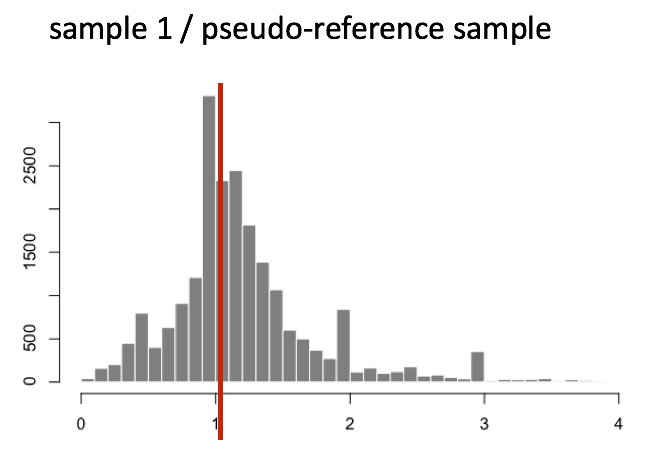
\includegraphics[width=4.16667in,height=\textheight,keepaspectratio]{img/deseq_median_of_ratios.png}

This method is robust as it assumes that not all genes are differentially expressed, allowing normalization factors to account for both sequencing depth and RNA composition efficiently.

\textbf{Step 4: Calculate the Normalized Count Values Using the Normalization Factor}

Each raw count value in a given sample is divided by that sample's normalization factor to generate normalized count values across all genes:

\begin{longtable}[]{@{}lcc@{}}
\toprule\noalign{}
Gene & Sample A & Sample B \\
\midrule\noalign{}
\endhead
\bottomrule\noalign{}
\endlastfoot
EF2A & 1489 / 1.3 = \textbf{1145.39} & 906 / 0.77 = \textbf{1176.62} \\
ABCD1 & 22 / 1.3 = \textbf{16.92} & 13 / 0.77 = \textbf{16.88} \\
\ldots{} & \ldots{} & \ldots{} \\
\end{longtable}

\begin{quote}
Note that normalized count values may not always be whole numbers.
\end{quote}

\subsection{Summary of Key Reasons for Using DESeq2}\label{summary-of-key-reasons-for-using-deseq2}

\begin{itemize}
\item
  \textbf{Median of Ratios}: This method accounts for sequencing depth and RNA composition, making it more appropriate for RNA-Seq data analysis.
\item
  \textbf{Geometric Mean}: It creates a pseudo-reference that reduces sensitivity to extreme values, affording more stable estimates.
\item
  \textbf{Normalization Procedures}: It ensures reliable comparisons of gene expression across samples by mitigating bias from technical variations, leading to more accurate differential expression analysis.
\end{itemize}

This combination of methodologies allows DESeq2 to provide robust results, enhancing the identification of differentially expressed genes in complex biological datasets.

\textbf{Exercise} points = +1

Determine the normalized counts for your gene of interest, PD1, given the raw counts and size factors below.

NOTE: You will need to run the code below to generate the raw counts dataframe (PD1) and the size factor vector (size\_factors), then use these objects to determine the normalized counts values:

\begin{lstlisting}[language=R]
# Raw counts for PD1
PD1 <- c(21, 58, 17, 97, 83, 10)
names(PD1) <- paste0("Sample", 1:6)
PD1 <- data.frame(PD1)
PD1 <- t(PD1)

# Size factors for each sample
size_factors <- c(1.32, 0.7, 1.04, 1.27, 1.11, 0.85)
\end{lstlisting}

\begin{lstlisting}[language=R]
# Your code here
\end{lstlisting}

\begin{center}\rule{0.5\linewidth}{0.5pt}\end{center}

\section{Count normalization of Mov10}\label{count-normalization-of-mov10}

Now that we know the theory of count normalization, we will normalize the counts for the Mov10 dataset using DESeq2. This requires a few steps:

\begin{enumerate}
\def\labelenumi{\arabic{enumi}.}
\tightlist
\item
  Ensure the row names of the metadata dataframe are present and in the same order as the column names of the counts dataframe.
\item
  Create a \passthrough{\lstinline!DESeqDataSet!} object
\item
  Generate the normalized counts
\end{enumerate}

\subsection{1. Match the metadata and counts data}\label{match-the-metadata-and-counts-data}

We should always make sure that we have sample names that match between the two files, and that the samples are in the right order. DESeq2 will output an error if this is not the case.

\begin{lstlisting}[language=R]
### Check that sample names match in both files
all(colnames(data) %in% rownames(meta))
\end{lstlisting}

\section{{[}1{]} TRUE}\label{true}

\begin{lstlisting}[language=R]
all(colnames(data) == rownames(meta))
\end{lstlisting}

\section{{[}1{]} FALSE}\label{false}

The colnames of our data don't match the rownames of our metadata so we need to reorder them. We can use the \passthrough{\lstinline!match!} function:

\begin{lstlisting}[language=R]
idx <- match(rownames(meta), colnames(data))
data <- data[, idx]

all(colnames(data) == rownames(meta))
\end{lstlisting}

\section{{[}1{]} TRUE}\label{true-1}

\textbf{Exercise} points = +2

Suppose we had sample names matching in the counts matrix and metadata file, but they were out of order. Write the line(s) of code required to create a new matrix with columns ordered such that they were identical to the row names of the metadata.

\begin{lstlisting}[language=R]
# write the code to reorder the columns of the 'counts' matrix to match the
# rownames of the metadata

# check that the rownames of the metadata match the colnames of the 'counts'
# matrix
\end{lstlisting}

\begin{center}\rule{0.5\linewidth}{0.5pt}\end{center}

\subsection{2. Create DESEq2 object}\label{create-deseq2-object}

Bioconductor software packages often define and use a custom class within R for storing data (input data, intermediate data and also result data). These custom data structures are similar to \passthrough{\lstinline!lists!} in that they can contain multiple different data types/structures within them. But, unlike lists they have pre-specified \passthrough{\lstinline!data slots!}, which hold specific types/classes of data. The data stored in these pre-specified slots can be accessed by using specific package-defined functions.

Let's start by creating the \passthrough{\lstinline!DESeqDataSet!} object and then we can talk a bit more about what is stored inside it. To create the object we will need the \textbf{count matrix} and the \textbf{metadata} table as input. We will also need to specify a \textbf{design formula}. The design formula specifies the column(s) in the metadata table and how they should be used in the analysis. For our dataset we only have one column we are interested in, that is \passthrough{\lstinline!\~sampletype!}. This column has three factor levels, which tells DESeq2 that for each gene we want to evaluate gene expression change with respect to these different levels.

\begin{lstlisting}[language=R]
## Create DESeq2Dataset object
dds <- DESeqDataSetFromMatrix(countData = data, colData = meta, design = ~sampletype)
\end{lstlisting}

\pandocbounded{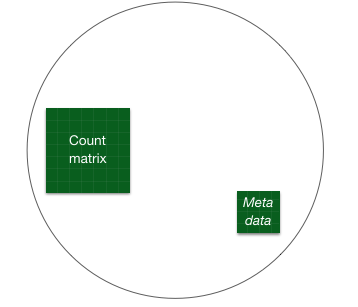
\includegraphics[keepaspectratio]{img/deseq_obj1.png}}

You can use DESeq-specific functions to access the different slots and retrieve information, if you wish. For example, suppose we wanted the original count matrix we would use \passthrough{\lstinline!counts()!}:

\begin{lstlisting}[language=R]
head(counts(dds[, 1:5]))
\end{lstlisting}

\section{Irrel\_kd\_1 Irrel\_kd\_2 Irrel\_kd\_3 Mov10\_kd\_2 Mov10\_kd\_3}\label{irrel_kd_1-irrel_kd_2-irrel_kd_3-mov10_kd_2-mov10_kd_3-1}

\section{1/2-SBSRNA4 45 31 39 57 41}\label{sbsrna4-45-31-39-57-41}

\section{A1BG 77 58 40 71 40}\label{a1bg-77-58-40-71-40}

\section{A1BG-AS1 213 172 126 256 177}\label{a1bg-as1-213-172-126-256-177}

\section{A1CF 0 0 0 0 1}\label{a1cf-0-0-0-0-1}

\section{A2LD1 91 80 50 146 81}\label{a2ld1-91-80-50-146-81}

\section{A2M 9 8 4 10 9}\label{a2m-9-8-4-10-9}

As we go through the workflow we will use the relevant functions to check what information gets stored inside our object. We can also run:

\begin{lstlisting}[language=R]
slotNames(dds)
\end{lstlisting}

\section{{[}1{]} ``design'' ``dispersionFunction'' ``rowRanges''}\label{design-dispersionfunction-rowranges}

\section{{[}4{]} ``colData'' ``assays'' ``NAMES''}\label{coldata-assays-names}

\section{{[}7{]} ``elementMetadata'' ``metadata''}\label{elementmetadata-metadata}

\subsection{3. Generate the Mov10 normalized counts}\label{generate-the-mov10-normalized-counts}

The next step is to normalize the count data in order to be able to make fair gene comparisons between samples.

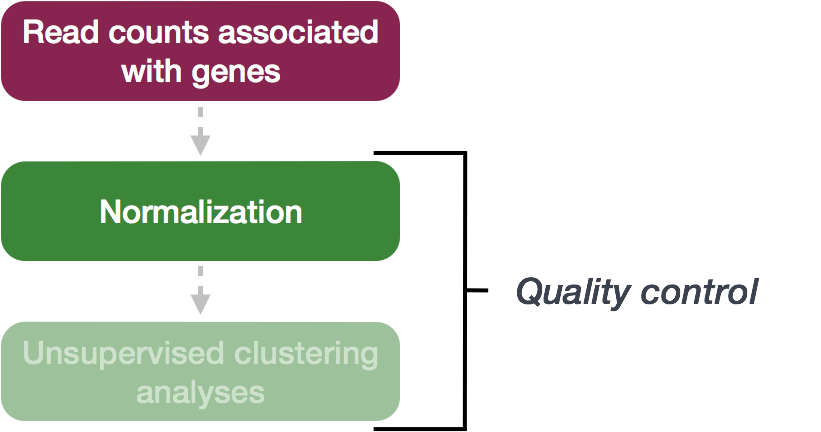
\includegraphics[width=4.16667in,height=\textheight,keepaspectratio]{img/deseq_workflow_normalization_2018.png}

To perform the \textbf{median of ratios method} of normalization, DESeq2 has a single \passthrough{\lstinline!estimateSizeFactors()!} function that will generate size factors for us. We will use the function in the example below, but \textbf{in a typical RNA-seq analysis this step is automatically performed by the \passthrough{\lstinline!DESeq()!} function}, which we will see later.

\begin{lstlisting}[language=R]
dds <- estimateSizeFactors(dds)
\end{lstlisting}

By assigning the results back to the \passthrough{\lstinline!dds!} object we are filling in the slots of the \passthrough{\lstinline!DESeqDataSet!} object with the appropriate information. We can take a look at the normalization factor applied to each sample using:

\begin{lstlisting}[language=R]
sizeFactors(dds)
\end{lstlisting}

\section{Irrel\_kd\_1 Irrel\_kd\_2 Irrel\_kd\_3 Mov10\_kd\_2 Mov10\_kd\_3 Mov10\_oe\_1 Mov10\_oe\_2}\label{irrel_kd_1-irrel_kd_2-irrel_kd_3-mov10_kd_2-mov10_kd_3-mov10_oe_1-mov10_oe_2}

\section{1.1224020 0.9625632 0.7477715 1.5646728 0.9351760 1.2016082 1.1205912}\label{section}

\section{Mov10\_oe\_3}\label{mov10_oe_3}

\section{0.6534987}\label{section-1}

Now, to retrieve the normalized counts matrix from \passthrough{\lstinline!dds!}, we use the \passthrough{\lstinline!counts()!} function and add the argument \passthrough{\lstinline!normalized=TRUE!}.

\begin{lstlisting}[language=R]
normalized_counts <- counts(dds, normalized = TRUE)
\end{lstlisting}

We can save this normalized data matrix to file for later use:

\begin{lstlisting}[language=R]
write.table(normalized_counts, file = "data/normalized_counts.txt", sep = "\t", quote = F,
    col.names = NA)
\end{lstlisting}

\chapter{Quality Control}\label{quality-control}

The next step in the DESeq2 workflow is QC, which includes sample-level and gene-level steps to perform QC checks on the count data to help us ensure that the samples/replicates look good.

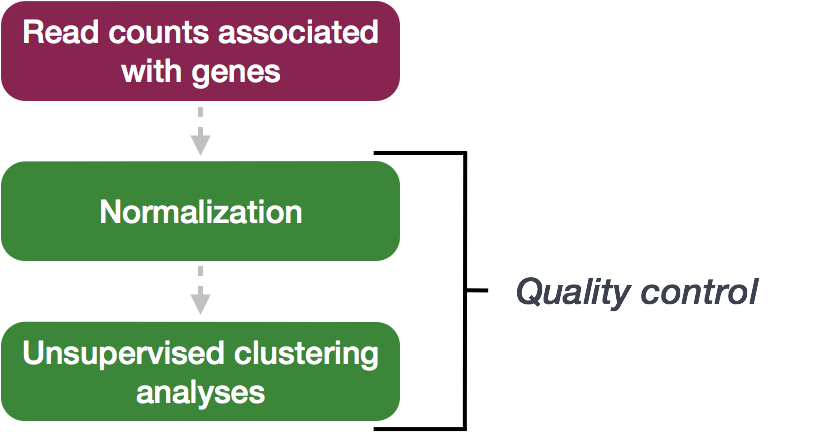
\includegraphics[width=4.16667in,height=\textheight,keepaspectratio]{img/deseq_workflow_qc_2018.png}

\section{Sample-level QC}\label{sample-level-qc}

A useful initial step in an RNA-seq analysis is often to assess overall similarity between samples:

\begin{itemize}
\tightlist
\item
  Which samples are similar to each other, which are different?
\item
  Does this fit to the expectation from the experiment's design?
\item
  What are the major sources of variation in the dataset?
\end{itemize}

To explore the similarity of our samples, we will be performing sample-level QC using Principal Component Analysis (PCA) and hierarchical clustering methods. Our sample-level QC allows us to see how well our replicates cluster together, as well as, observe whether our experimental condition represents the major source of variation in the data. Performing sample-level QC can also identify any sample outliers, which may need to be explored further to determine whether they need to be removed prior to DE analysis.

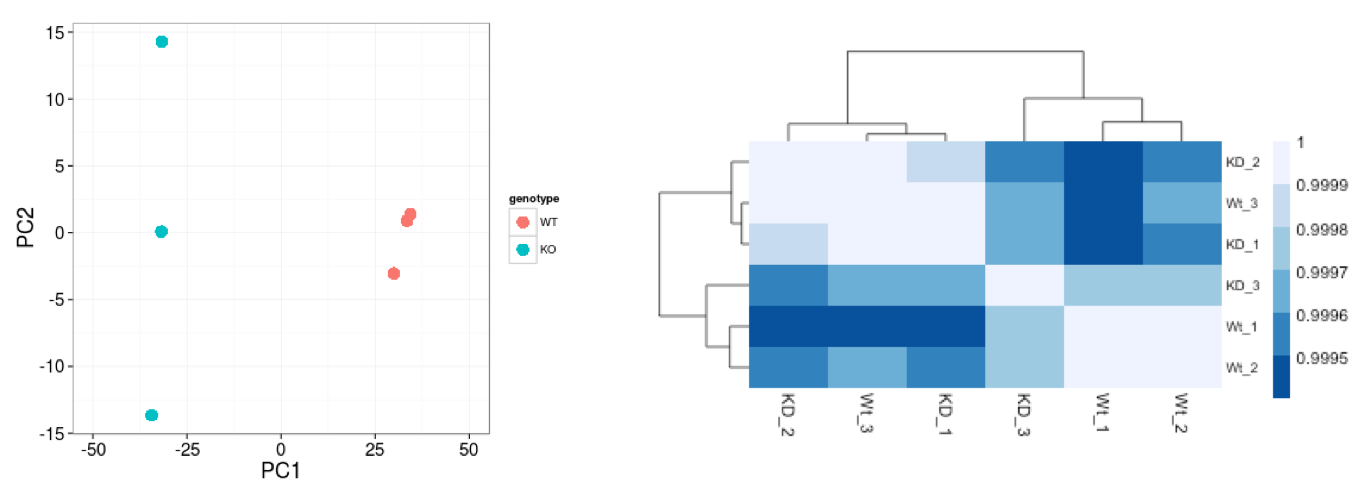
\includegraphics[width=7.29167in,height=\textheight,keepaspectratio]{img/sample_qc.png}

When using these unsupervised clustering methods, log2-transformation of the normalized counts improves the distances/clustering for visualization. DESeq2 uses a \textbf{regularized log transform} (rlog) of the normalized counts for sample-level QC as it moderates the variance across the mean, improving the clustering.

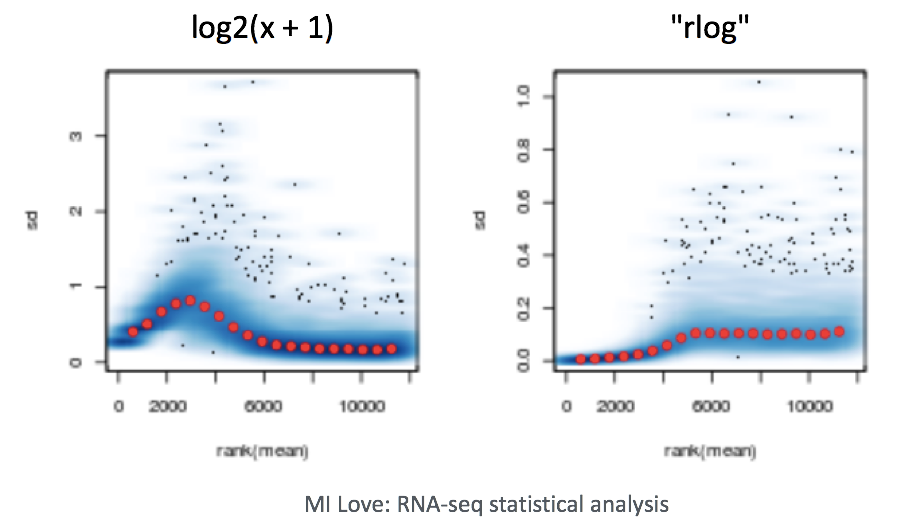
\includegraphics[width=5.20833in,height=\textheight,keepaspectratio]{img/rlog_transformation.png}

Principal Component Analysis (PCA) is a technique used to emphasize variation and highlight strong patterns in a dataset. It is particularly useful for dimensionality reduction, meaning it simplifies large datasets by identifying the directions (or principal components) that explain the greatest variation in the data. For a more detailed introduction to PCA, we recommend watching this \href{https://www.youtube.com/watch?v=_UVHneBUBW0}{StatQuest's video}.

Suppose we have a dataset with two samples and four genes. To evaluate the relationship between these samples, we can plot the counts of one sample against the other, with Sample 1 on the x-axis and Sample 2 on the y-axis, as shown below:

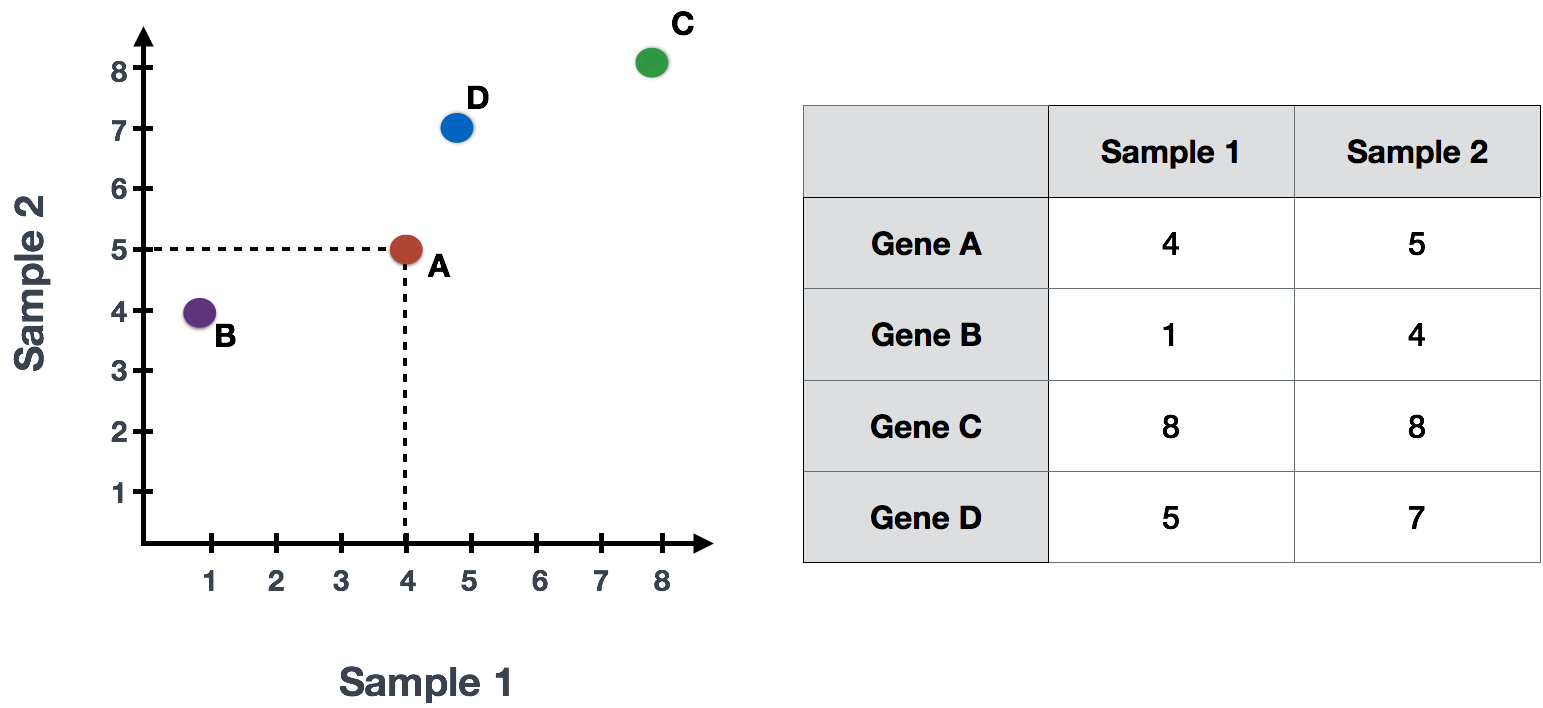
\includegraphics[width=6.25in,height=\textheight,keepaspectratio]{img/PCA_2sample_genes.png}

For PCA analysis, the first step is finding the \textbf{first principal component} (PC1). The \textbf{first principal component} is the direction that \textbf{maximizes the variance} (the sum of squared distances from the mean) and simultaneously \textbf{minimizes the squared distances between the data points} and their projections onto that line. Why? Because variance is essentially the spread (or squared distances) of the data from its mean, and PCA wants to capture as much of this spread as possible. In this example, the most variation is along the diagonal. That is, the \textbf{largest spread in the data} is between the two endpoints of this line. \textbf{This is called the first principal component, or PC1.} The genes at the endpoints of this line (Gene B and Gene C) have the \textbf{greatest influence} on the direction of this line.

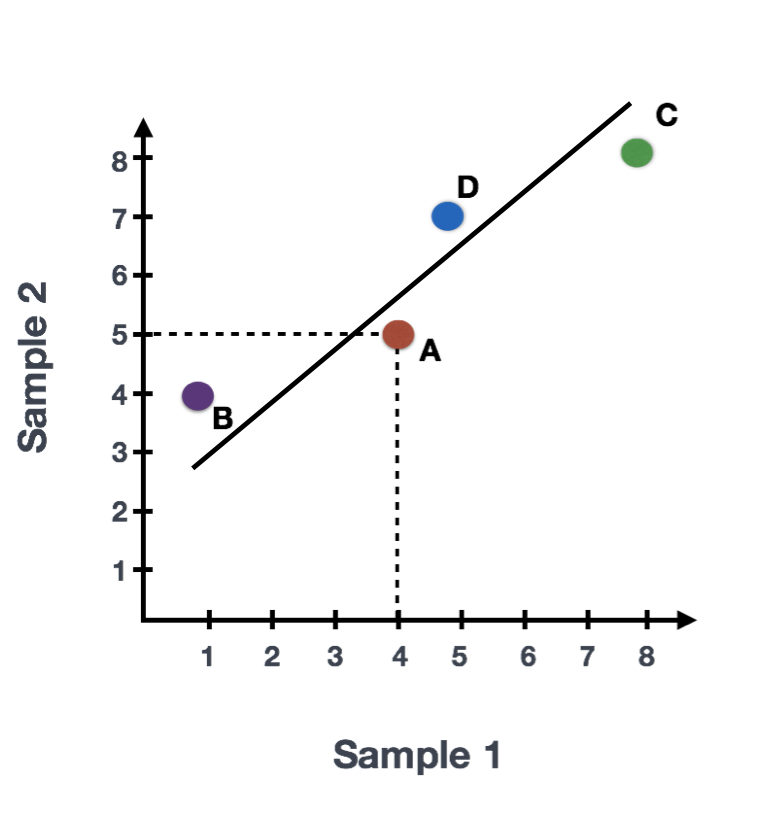
\includegraphics[width=3.125in,height=\textheight,keepaspectratio]{img/pca_with_PC1_line.png}

After determining PC1, PCA assigns each sample a \textbf{PC1 score}, which represents how each sample aligns with this principal component. The score for each sample is calculated by taking the product of each gene's influence on PC1 and its normalized expression in the sample, and summing these products across all genes. A second line can then be drawn to represent the \textbf{second principal component (PC2)}, which captures the second-largest amount of variation in the data. This process can continue for additional principal components.

The formula to calculate a sample's PC1 score is as follows:

\[
\text{Sample1 PC1 score} = \sum_{i=1}^{n} (\text{counts}_{i} \times \text{influence}_{i})
\]

Where:

\begin{itemize}
\item
  \(\text{counts}_{i}\): Normalized expression of gene \(i\) in the sample
\item
  \(\text{influence}_{i}\): Influence of gene \(i\) on PC1
\end{itemize}

While calculating the \textbf{influence} of each gene on PC1 is complex, a key step involves calculating a z-score for each gene.

A z-score measures how far a gene's expression deviates from the mean, and genes with larger z-scores (like Gene B and Gene C in this example) have a greater influence on PC1 because they contribute more to the variation.

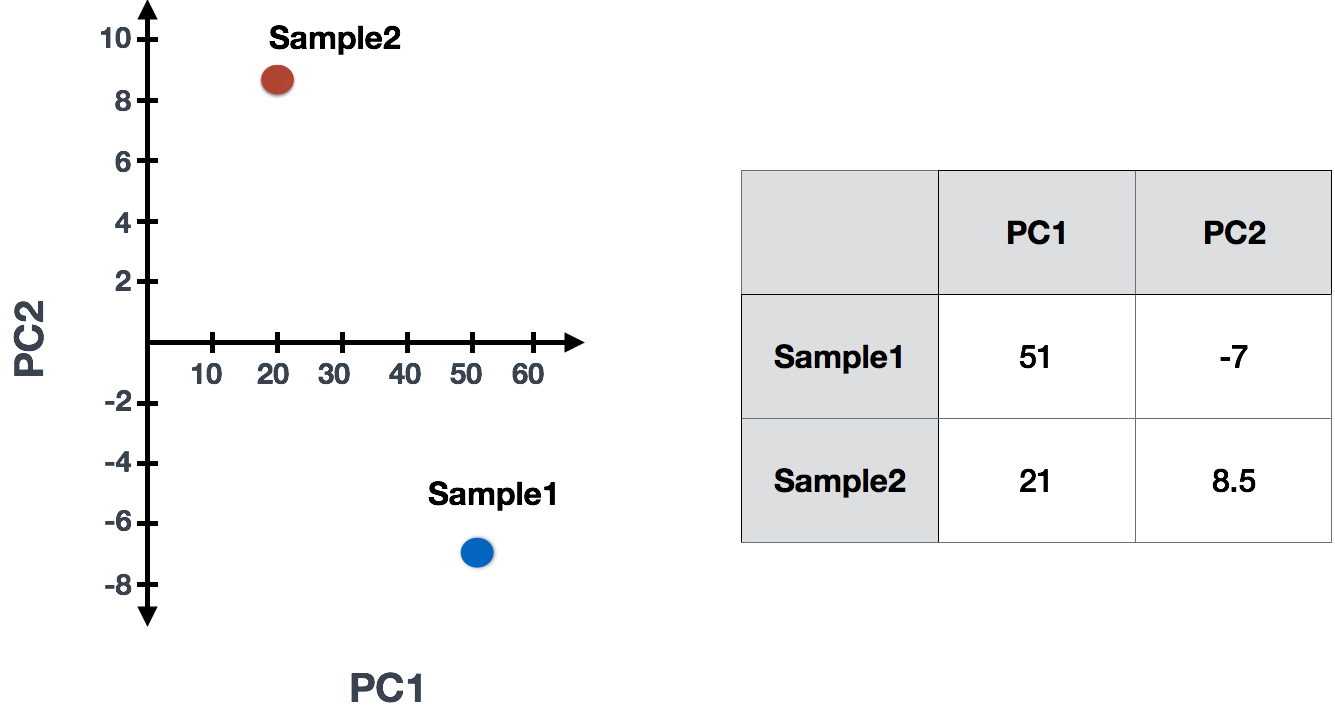
\includegraphics[width=6.25in,height=\textheight,keepaspectratio]{img/PCA_samples.png}

Briefly, calculating PCA and the influence of each gene on PC1 involves the following steps:

\subsubsection{Steps to calculate PCA}\label{steps-to-calculate-pca}

\begin{enumerate}
\def\labelenumi{\arabic{enumi}.}
\tightlist
\item
  \textbf{Z-Scores}:
\end{enumerate}

\begin{itemize}
\tightlist
\item
  A z-score transforms the data points, indicating how far a value is from the mean in terms of standard deviations. This standardization adjusts for differences in scale between different genes, allowing for more accurate comparisons.
\item
  The formula for calculating a z-score for a value \(x\) of a gene is:
\end{itemize}

\[
z = \frac{x - \mu}{\sigma}
\]

Where:

\begin{itemize}
\item
  \(\mu\) is the mean expression of the gene across samples.
\item
  \(\sigma\) is the standard deviation of the gene expression.
\end{itemize}

\begin{enumerate}
\def\labelenumi{\arabic{enumi}.}
\setcounter{enumi}{1}
\tightlist
\item
  \textbf{Covariance matrix}:
\end{enumerate}

\begin{itemize}
\item
  Covariance measures the degree to which two variables change together. In the context of PCA, we calculate the covariance matrix for standardized (z-scored) gene expressions to understand how genes vary together.
\item
  A positive covariance indicates that higher values of one gene correspond to higher values of another, while a negative covariance implies that higher values of one gene correspond to lower values of another.
\item
  After standardizing the data, calculate the covariance between the z-scores of different genes. This will produce a covariance matrix that reveals how gene expressions vary together.
\item
  In the context of Principal Component Analysis (PCA), the covariance matrix is a crucial component. It captures how variables in the dataset change with respect to one another and is used to determine the principal components.
\end{itemize}

\begin{enumerate}
\def\labelenumi{\arabic{enumi}.}
\setcounter{enumi}{2}
\tightlist
\item
  \textbf{Eigenvectors and Eigenvalues:} Find these from the covariance matrix. They reveal the directions (principal components) and their importance (variance explained) in the data. Think of PCA as creating new ``axes'' or dimensions that capture the most variation in the data. PCA will identify the direction of these axes based on the covariance of the standardized gene expressions that better highlight differences in your data.
\end{enumerate}

The \textbf{take-home message} is that if \textbf{two samples have similar levels of expression for the genes that contribute significantly to PC1}, they will have similar PC1 scores and will be plotted close to each other on the PC1 axis. Therefore, we would expect \textbf{biological replicates} (samples from the same condition) to have similar PC1 scores and cluster together. On the other hand, samples from different treatment groups should have different PC1 scores, reflecting their distinct gene expression patterns. This is more easily understood through visualizing example PCA plots.

\subsubsection{Interpreting PCA plots}\label{interpreting-pca-plots}

In real datasets with many samples and genes, PCA reduces the complex, high-dimensional data into a 2-dimensional space, where each sample is represented by its scores for the principal components. Typically, we plot the first two principal components (PC1 and PC2), as they explain the most variation in the data.

When interpreting PCA plots, \textbf{biological replicates} (samples from the same condition) should cluster together because they have similar expression patterns for the genes driving variation in PC1. \textbf{Samples from different treatment groups} will often separate along these axes, reflecting differences in their gene expression profiles.

This is best understood by looking at example PCA plots, where you can visualize how biological replicates cluster and treatment groups separate based on their gene expression patterns.

\subsubsection{Interpreting PCA plots example}\label{interpreting-pca-plots-example}

We have an example dataset and a few associated PCA plots below to get a feel for how to interpret them. The metadata for the experiment is displayed below. The main condition of interest is \passthrough{\lstinline!treatment!}.

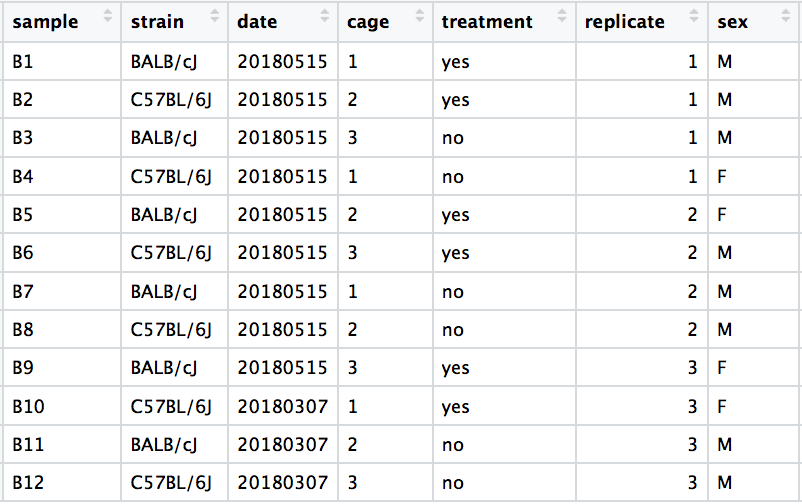
\includegraphics[width=6.25in,height=\textheight,keepaspectratio]{img/example_metadata.png}

When visualizing the samples on PC1 and PC2, we can color the points based on different metadata columns to identify potential sources of variation. In the first plot, if we don't observe a clear separation of samples by \passthrough{\lstinline!treatment!}, we can explore other factors that may explain the variation. Ideally, our metadata table includes all known sources of variation (such as batch effects, age, or gender), and we can use these factors to color the PCA plot to see if they explain any underlying patterns.

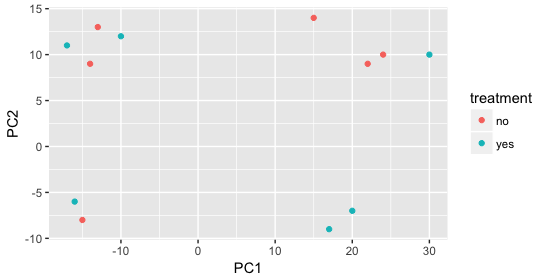
\includegraphics[width=6.25in,height=\textheight,keepaspectratio]{img/example_PCA_treatmentPC1.png}

We begin by coloring the points in the PCA plot based on the \passthrough{\lstinline!cage!} factor, but this factor does not seem to explain the variation observed on PC1 or PC2.

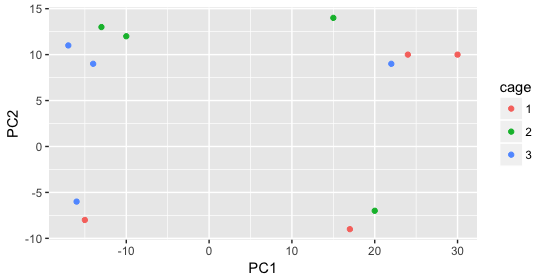
\includegraphics[width=6.25in,height=\textheight,keepaspectratio]{img/example_PCA_cage.png}

Next, we color the points by the \passthrough{\lstinline!sex!} factor. Here, we observe that \passthrough{\lstinline!sex!} separates the samples along PC2, which is valuable information. We can use this in our model to account for variation due to \passthrough{\lstinline!sex!} and potentially regress it out to focus on other sources of variation.

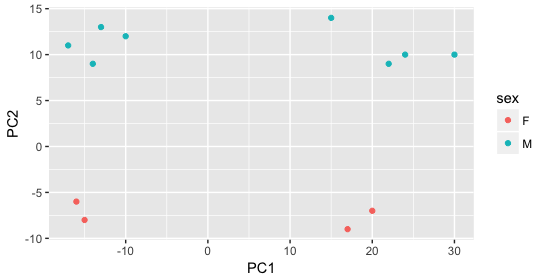
\includegraphics[width=6.25in,height=\textheight,keepaspectratio]{img/example_PCA_sex.png}

Next we explore the \passthrough{\lstinline!strain!} factor and find that it explains the variation on PC1.

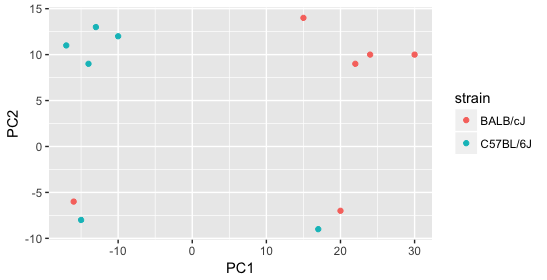
\includegraphics[width=6.25in,height=\textheight,keepaspectratio]{img/example_PCA_strain.png}

It's great that we have been able to identify the sources of variation for both PC1 and PC2. By accounting for it in our model, we should be able to detect more genes differentially expressed due to \passthrough{\lstinline!treatment!}.

Worrisome about this plot is that we see two samples that do not cluster with the correct strain. This would indicate a likely \textbf{sample swap} and should be investigated to determine whether these samples are indeed the labeled strains. If we found there was a switch, we could swap the samples in the metadata. However, if we think they are labeled correctly or are unsure, we could just remove the samples from the dataset.

Still we haven't found if \passthrough{\lstinline!treatment!} is a major source of variation after \passthrough{\lstinline!strain!} and \passthrough{\lstinline!sex!}. So, we explore PC3 and PC4 to see if \passthrough{\lstinline!treatment!} is driving the variation represented by either of these PCs.

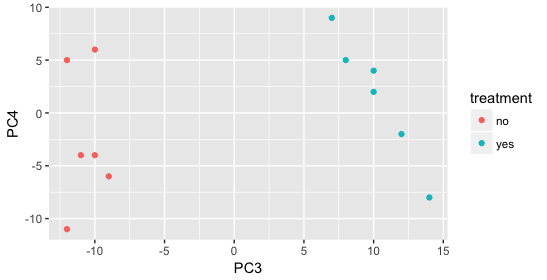
\includegraphics[width=6.25in,height=\textheight,keepaspectratio]{img/example_PCA_treatmentPC3.png}

We find that the samples separate by \passthrough{\lstinline!treatment!} on PC3, and are optimistic about our DE analysis since our condition of interest, \passthrough{\lstinline!treatment!}, is separating on PC3 and we can regress out the variation driving PC1 and PC2. Treatment separating on PC3 indicates that it still contributes to variation, but its effect is smaller and is only captured after accounting for the larger effects (\passthrough{\lstinline!strain!}, \passthrough{\lstinline!sex!})..
me stop

\textbf{Exercise} points = +5

The figure below was generated from a time course experiment with sample groups `Ctrl' and `Sci' and the following timepoints: 0h, 2h, 8h, and 16h.

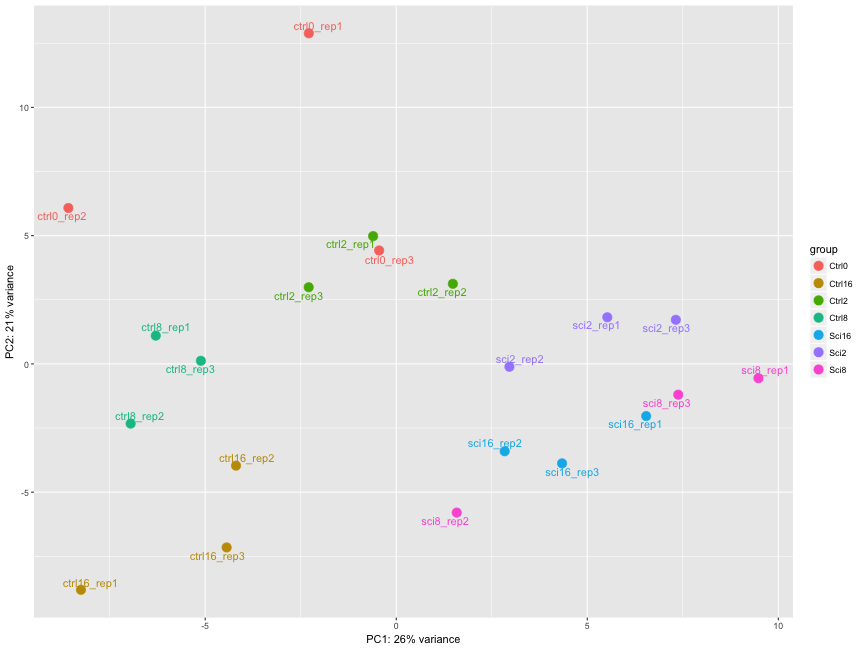
\includegraphics[width=6.25in,height=\textheight,keepaspectratio]{img/PCA_example3.png}

\textbf{Determine the sources explaining the variation represented by PC1 and PC2.}

\begin{itemize}
\tightlist
\item
  Ans:
\end{itemize}

\textbf{Do the sample groups separate well?}

\begin{itemize}
\tightlist
\item
  Ans:
\end{itemize}

\textbf{Do the replicates cluster together for each sample group?}

\begin{itemize}
\tightlist
\item
  Ans:
\end{itemize}

\textbf{Are there any outliers in the data?}

\begin{itemize}
\tightlist
\item
  Ans:
\end{itemize}

\textbf{Should we have any other concerns regarding the samples in the dataset?}

\begin{itemize}
\tightlist
\item
  Ans:
\end{itemize}

\subsection{Recommended Resources}\label{recommended-resources}

For further reading and visual examples of PCA, consider resources such as:
- StatQuest's PCA video (\href{https://www.youtube.com/watch?v=_UVHneBUBW0}{Link})
- Online tutorials on PCA in bioinformatics.

\subsection{Hierarchical Clustering Heatmap}\label{hierarchical-clustering-heatmap}

Similar to PCA, hierarchical clustering is another, complementary method for identifying strong patterns in a dataset and potential outliers. The heatmap displays \textbf{the correlation of gene expression for all pairwise combinations of samples} in the dataset. Since the majority of genes are not differentially expressed, samples generally have high correlations with each other (values higher than 0.80). Samples below 0.80 may indicate an outlier in your data and/or sample contamination.

The hierarchical tree can indicate which samples are more similar to each other based on the normalized gene expression values. The color blocks indicate substructure in the data, and you would expect to see your replicates cluster together as a block for each sample group. Additionally, we expect to see samples clustered similar to the groupings observed in a PCA plot.

\textbf{In the plot below, we would be quite concerned about `Wt\_3' and `KD\_3' samples not clustering with the other replicates. We would want to explore the PCA to see if we see the same clustering of samples.}

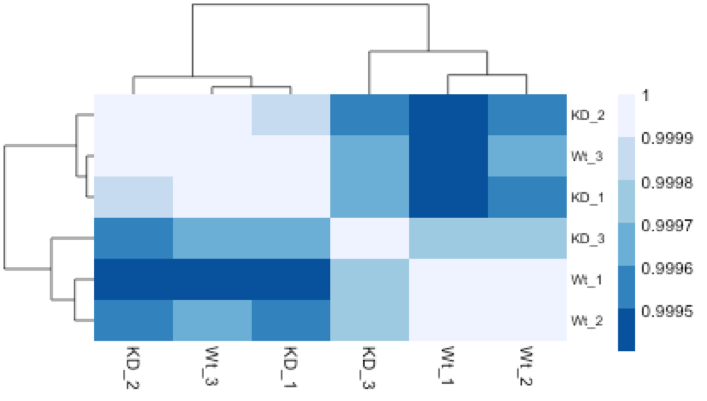
\includegraphics[width=5.20833in,height=\textheight,keepaspectratio]{img/heatmap_example.png}

\section{Gene-level QC}\label{gene-level-qc}

In addition to examining how well the samples/replicates cluster together, there are a few more QC steps. Prior to differential expression analysis it is beneficial to omit genes that have little or no chance of being detected as differentially expressed. This will increase the power to detect differentially expressed genes. The genes omitted fall into three categories:

\begin{itemize}
\tightlist
\item
  Genes with zero counts in all samples
\item
  Genes with an extreme count outlier
\item
  Genes with a low mean normalized counts
\end{itemize}

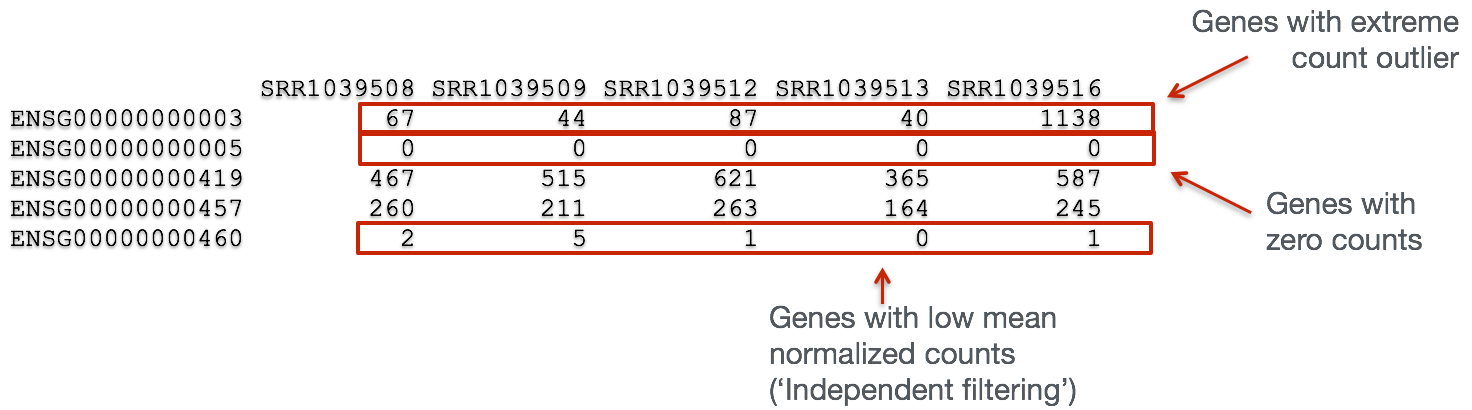
\includegraphics[width=6.25in,height=\textheight,keepaspectratio]{img/gene_filtering.png}

\textbf{DESeq2 will perform this filtering by default; however other DE tools, such as EdgeR will not.} Filtering is a necessary step, especially when you are using methods other than DESeq2.

\section{Mov10 quality assessment and exploratory analysis using DESeq2}\label{mov10-quality-assessment-and-exploratory-analysis-using-deseq2}

Now that we have a good understanding of the QC steps normally employed for RNA-seq, let's implement them for the Mov10 dataset we are going to be working with.

\subsection{Transform normalized counts using the rlog transformation}\label{transform-normalized-counts-using-the-rlog-transformation}

\textbf{To improve the distances/clustering for the PCA and heirarchical clustering visualization methods}, we need to apply the \textbf{regularized log transformation (rlog)} transformation to the normalized counts. \textbf{rlog} is used for visualizations in RNA-Seq data analysis, particularly with tools like DESeq2, because it stabilizes the variance across different levels of gene expression, making it easier to interpret patterns in the data.

\textbf{Example of Variance Stabilization}
Raw RNA-Seq count data has different levels of variability:

Without stabilization: Lowly expressed genes show high variability between samples (often due to noise), and highly expressed genes show less variability.
With stabilization (e.g., rlog or vst): Variance across genes is more evenly distributed, which makes the data easier to work with in analyses like clustering or PCA.

\begin{quote}
The rlog transformation of the normalized counts is only necessary for these visualization methods during this quality assessment.
\end{quote}

\begin{lstlisting}[language=R]
### Transform counts for data visualization
rld <- rlog(dds, blind = TRUE)
\end{lstlisting}

The \passthrough{\lstinline!blind=TRUE!} argument results in a transformation unbiased to sample condition information. When performing quality assessment, it is important to include this option. The \href{http://bioconductor.org/packages/devel/bioc/vignettes/DESeq2/inst/doc/DESeq2.html\#blind-dispersion-estimation}{DESeq2 vignette} has more details.

The \passthrough{\lstinline!rlog!} function returns a \passthrough{\lstinline!DESeqTransform!} object, another type of DESeq-specific object. The reason you don't just get a matrix of transformed values is because all of the parameters (i.e.~size factors) that went into computing the rlog transform are stored in that object. We use this object to plot the PCA and heirarchical clustering figures for quality assessment.

\subsection{Principal components analysis (PCA)}\label{principal-components-analysis-pca}

DESeq2 has a built-in function for plotting PCA plots, that uses \passthrough{\lstinline!ggplot2!} under the hood. This is great because it saves us having to type out lines of code and having to fiddle with the different ggplot2 layers. In addition, it takes the \passthrough{\lstinline!rlog!} object as an input directly, hence saving us the trouble of extracting the relevant information from it.

The function \passthrough{\lstinline!plotPCA()!} requires two arguments as input: an \passthrough{\lstinline!rlog!} object and the \passthrough{\lstinline!intgroup!} (the column in our metadata that we are interested in).

\begin{lstlisting}[language=R]
### Plot PCA
plotPCA(rld, intgroup = "sampletype")
\end{lstlisting}

\begin{center}\includegraphics{2025_RNA-Seq-Analysis_files/figure-latex/unnamed-chunk-25-1} \end{center}

\textbf{What does this plot tell you about the similarity of samples? Does it fit the expectation from the experimental design?} By default the function uses the \emph{top 500 most variable genes}. You can change this by adding the \passthrough{\lstinline!ntop!} argument and specifying how many genes you want to use to draw the plot.

\begin{quote}
\href{http://www.sthda.com/english/wiki/principal-component-analysis-in-r-prcomp-vs-princomp-r-software-and-data-mining}{Resources} are available to learn how to do more complex inquiries using the PCs.
\end{quote}

\subsection{Hierarchical Clustering}\label{hierarchical-clustering}

Since there is no built-in function for heatmaps in DESeq2 we will be using the \passthrough{\lstinline!pheatmap()!} function from the \passthrough{\lstinline!pheatmap!} package. This function requires a matrix/dataframe of numeric values as input, and so the first thing we need to is retrieve that information from the \passthrough{\lstinline!rld!} object:

\begin{lstlisting}[language=R]
### Extract the rlog matrix from the object
rld_mat <- assay(rld)  ## assay() is function from the 'SummarizedExperiment' package that was loaded when you loaded DESeq2
\end{lstlisting}

Then we need to compute the pairwise correlation values for samples. We can do this using the \passthrough{\lstinline!cor()!} function:

\begin{lstlisting}[language=R]
### Compute pairwise correlation values
rld_cor <- cor(rld_mat)  ## cor() is a base R function

head(rld_cor)  ## check the output of cor(), make note of the rownames and colnames
\end{lstlisting}

\section{Irrel\_kd\_1 Irrel\_kd\_2 Irrel\_kd\_3 Mov10\_kd\_2 Mov10\_kd\_3 Mov10\_oe\_1}\label{irrel_kd_1-irrel_kd_2-irrel_kd_3-mov10_kd_2-mov10_kd_3-mov10_oe_1}

\section{Irrel\_kd\_1 1.0000000 0.9999614 0.9999532 0.9997202 0.9997748 0.9996700}\label{irrel_kd_1-1.0000000-0.9999614-0.9999532-0.9997202-0.9997748-0.9996700}

\section{Irrel\_kd\_2 0.9999614 1.0000000 0.9999544 0.9996918 0.9997568 0.9996984}\label{irrel_kd_2-0.9999614-1.0000000-0.9999544-0.9996918-0.9997568-0.9996984}

\section{Irrel\_kd\_3 0.9999532 0.9999544 1.0000000 0.9996816 0.9997574 0.9997067}\label{irrel_kd_3-0.9999532-0.9999544-1.0000000-0.9996816-0.9997574-0.9997067}

\section{Mov10\_kd\_2 0.9997202 0.9996918 0.9996816 1.0000000 0.9999492 0.9994868}\label{mov10_kd_2-0.9997202-0.9996918-0.9996816-1.0000000-0.9999492-0.9994868}

\section{Mov10\_kd\_3 0.9997748 0.9997568 0.9997574 0.9999492 1.0000000 0.9996154}\label{mov10_kd_3-0.9997748-0.9997568-0.9997574-0.9999492-1.0000000-0.9996154}

\section{Mov10\_oe\_1 0.9996700 0.9996984 0.9997067 0.9994868 0.9996154 1.0000000}\label{mov10_oe_1-0.9996700-0.9996984-0.9997067-0.9994868-0.9996154-1.0000000}

\section{Mov10\_oe\_2 Mov10\_oe\_3}\label{mov10_oe_2-mov10_oe_3}

\section{Irrel\_kd\_1 0.9996599 0.9995804}\label{irrel_kd_1-0.9996599-0.9995804}

\section{Irrel\_kd\_2 0.9996825 0.9996227}\label{irrel_kd_2-0.9996825-0.9996227}

\section{Irrel\_kd\_3 0.9997090 0.9996026}\label{irrel_kd_3-0.9997090-0.9996026}

\section{Mov10\_kd\_2 0.9994565 0.9993869}\label{mov10_kd_2-0.9994565-0.9993869}

\section{Mov10\_kd\_3 0.9995905 0.9995235}\label{mov10_kd_3-0.9995905-0.9995235}

\section{Mov10\_oe\_1 0.9999505 0.9999196}\label{mov10_oe_1-0.9999505-0.9999196}

And now to plot the correlation values as a heatmap:

\begin{lstlisting}[language=R]
### Plot heatmap
pheatmap(rld_cor)
\end{lstlisting}

\begin{center}\includegraphics{2025_RNA-Seq-Analysis_files/figure-latex/unnamed-chunk-28-1} \end{center}

Overall, we observe pretty high correlations across the board ( \textgreater{} 0.999) suggesting no outlying sample(s). Also, similar to the PCA plot you see the samples clustering together by sample group. Together, these plots suggest to us that the data are of good quality and we have the green light to proceed to differential expression analysis.

\textbf{Exercise} points = +3

The pheatmap function has a number of different arguments that we can alter from default values to enhance the aesthetics of the plot. Try adding the arguments \passthrough{\lstinline!color!}, \passthrough{\lstinline!border\_color!}, \passthrough{\lstinline!fontsize\_row!}, \passthrough{\lstinline!fontsize\_col!}, \passthrough{\lstinline!show\_rownames!} and \passthrough{\lstinline!show\_colnames!} to your pheatmap. How does your plot change (plot shown below)? Take a look through the help pages (?pheatmap) and identify what each of the added arguments is contributing to the plot.

Pheatmap for exercise:

\begin{lstlisting}[language=R]
library(pheatmap)
library(RColorBrewer)
heat.colors <- colorRampPalette(brewer.pal(9, "Blues"))(100)

pheatmap(rld_cor, color = colorRampPalette(brewer.pal(9, "Blues"))(100))
\end{lstlisting}

\begin{center}\includegraphics{2025_RNA-Seq-Analysis_files/figure-latex/unnamed-chunk-29-1} \end{center}

\begin{lstlisting}[language=R]
library(pheatmap)
library(RColorBrewer)

pheatmap(rld_cor)
\end{lstlisting}

\begin{center}\includegraphics{2025_RNA-Seq-Analysis_files/figure-latex/unnamed-chunk-30-1} \end{center}

\begin{lstlisting}[language=R]
library(pheatmap)
pheatmap(rld_cor)
\end{lstlisting}

\pandocbounded{\includegraphics[keepaspectratio]{2025_RNA-Seq-Analysis_files/figure-latex/unnamed-chunk-31-1.pdf}}

\pandocbounded{\includegraphics[keepaspectratio]{2025_RNA-Seq-Analysis_files/figure-latex/unnamed-chunk-32-1.pdf}}

\begin{lstlisting}[language=R]
# The color palette 'Blues' is a good choice for this heatmap
heat.colors <- brewer.pal(9, "Blues")

# Your code here
\end{lstlisting}

\begin{center}\rule{0.5\linewidth}{0.5pt}\end{center}

\chapter{DGE analysis workflow}\label{dge-analysis-workflow}

Differential expression analysis with DESeq2 involves multiple steps as displayed in the flowchart below in blue.

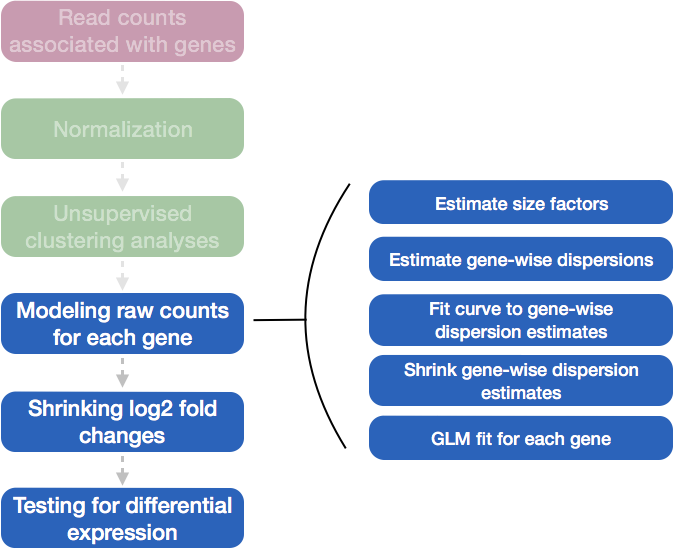
\includegraphics[width=6.25in,height=\textheight,keepaspectratio]{img/DESeq2_workflow_2018.png}
Here's a more succinct version of your workflow:

\textbf{DESeq2 Workflow Overview:}

\begin{enumerate}
\def\labelenumi{\arabic{enumi}.}
\item
  \textbf{Load Data:} Start with raw count data and sample metadata.
\item
  \textbf{Normalize Counts:} Estimate size factors to adjust for sequencing depth or library size differences.
\item
  \textbf{Estimate Dispersion:} Calculate gene-wise dispersion, measuring variability in counts not explained by mean expression.
\item
  \textbf{Fit Dispersion Trend:} Model the relationship between mean counts and dispersion, either parametrically (default) or non-parametrically.
\item
  \textbf{Shrink Dispersions:} Use empirical Bayes shrinkage to stabilize dispersion estimates, particularly for low-count genes. Empirical Bayes is a version of Bayesian statistics where the prior distribution is estimated from the data itself, rather than being set externally.
  In empirical Bayes shrinkage, the idea is to estimate a common pattern or distribution (the prior) across all observations (e.g., all genes) and then use this estimated distribution to influence or ``shrink'' each individual observation.
\item
  \textbf{Fit NB Model:} Fit a negative binomial model using the shrunken dispersion estimates, capturing variability and estimating log-fold changes.
\item
  \textbf{Shrink Log-Fold Changes:} Optionally stabilize log-fold changes with regularization, especially for low-expression genes.
\item
  \textbf{Statistical Testing:} Perform Wald tests to identify differentially expressed genes, providing adjusted p-values for multiple testing.
\end{enumerate}

This final step in the differential expression analysis workflow of fitting the raw counts to the \textbf{NB model} and performing the statistical test for differentially expressed genes, is the step we care about. This is the step that performs statistical tests to identify significant differences in gene expression between sample groups.

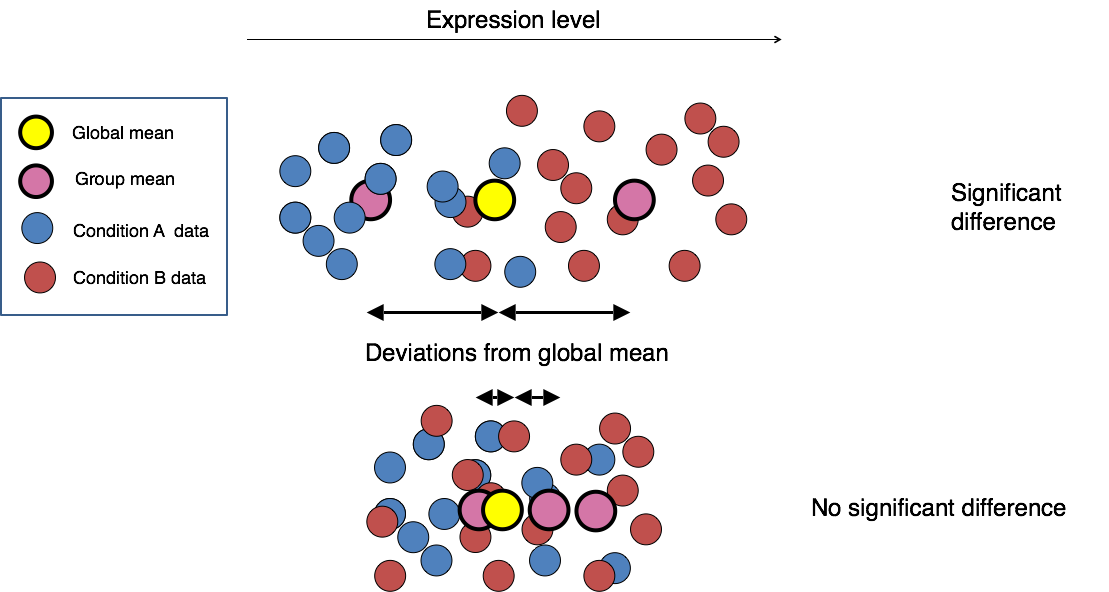
\includegraphics[width=6.25in,height=\textheight,keepaspectratio]{img/de_theory.png}

Although the \href{https://genomebiology.biomedcentral.com/articles/10.1186/s13059-014-0550-8}{DESeq2 paper} was published in 2014, but the package is continually updated and available for use in R through Bioconductor.

\section{Running DESeq2}\label{running-deseq2}

Prior to performing the differential expression analysis, it is a good idea to know what \textbf{sources of variation} are present in your data, either by exploration during the QC and/or prior knowledge. \textbf{Sources of variation} refer to anything that causes differences in gene expression across your samples, including \textbf{biological factors} (\textbf{treatment}, \textbf{sex}, \textbf{age}) and \textbf{technical factors} (\textbf{batch effects}, \textbf{sequencing depth}). Ideally, these are all factors in your metadata. These factors lead to variability in the data and can affect your ability to detect meaningful biological signals (like differential expression between \textbf{treated} and \textbf{control} samples).Once you know the major sources of variation, you can remove them prior to analysis or control for them in the statistical model by including them in your \textbf{design formula}.

\subsection{Set the Design Formula}\label{set-the-design-formula}

The main purpose of the \textbf{design formula} in DESeq2 is to specify the factors that are influencing gene expression so that their effects can be \textbf{accounted for} or \textbf{controlled} during the analysis. This allows DESeq2 to isolate the effect of the variable you're primarily interested in while adjusting for other known sources of variation. The design formula should have all of the factors in your metadata that account for major sources of variation in your data. The last factor entered in the formula should be the condition of interest.

For example:

\begin{lstlisting}[language=R]
design(dds)
\end{lstlisting}

\section{\textasciitilde sampletype}\label{sampletype}

This shows that \textbf{sampletype} is the condition of interest and as such is the only covariate. DESeq2 will test for differential expression between the two sample types, adjusting for any other variation.

\textbf{Example}

If you want to examine the expression differences between \passthrough{\lstinline!treatments!} as shown below, and you know that major sources of variation include \passthrough{\lstinline!sex!} and \passthrough{\lstinline!age!}, then your design formula would be:

\passthrough{\lstinline!design <- \~ sex + age + treatment!}

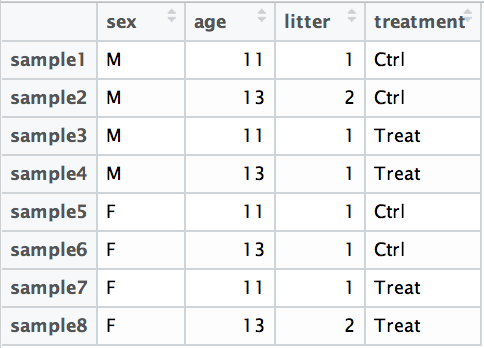
\includegraphics[width=3.125in,height=\textheight,keepaspectratio]{img/meta_example.png}

This allows DESeq2 to adjust for \textbf{sex} and \textbf{age} while testing for differences in \textbf{treatment}.

\textbf{Why is this important?}\\
Including known sources of variation (like \textbf{sex} and \textbf{age}) ensures any gene expression differences are due to the condition of interest (e.g., \textbf{treatment}), not confounded by other factors.

\textbf{Steps to set the design formula:}
1. Identify your factor of interest (e.g., \textbf{treatment}).
2. Determine any confounders (e.g., \textbf{sex}, \textbf{age}).
3. Write the formula, placing the factor of interest last.
4. Use \textbf{PCA} to ensure all relevant factors are included.

\textbf{Exercise} points = +3

\begin{enumerate}
\def\labelenumi{\arabic{enumi}.}
\tightlist
\item
  Suppose you wanted to study the expression differences between the two age groups in the metadata shown above, and major sources of variation were \textbf{sex} and \textbf{treatment}, how would the design formula be written?
\end{enumerate}

\begin{lstlisting}[language=R]
# Your code here
\end{lstlisting}

\begin{enumerate}
\def\labelenumi{\arabic{enumi}.}
\setcounter{enumi}{1}
\tightlist
\item
  Based on our Mov10 metadata dataframe, which factors could we include in our design formula?
\end{enumerate}

\begin{itemize}
\tightlist
\item
  Ans:
\end{itemize}

\begin{enumerate}
\def\labelenumi{\arabic{enumi}.}
\setcounter{enumi}{2}
\tightlist
\item
  What would you do if you wanted to include a factor in your design formula that is not in your metadata?
\end{enumerate}

\begin{itemize}
\tightlist
\item
  Ans:
\end{itemize}

\subsection{MOV10 Differential Expression Analysis}\label{mov10-differential-expression-analysis}

Now that we understand how to specify the model in DESeq2, we can proceed with running the differential expression pipeline on the raw count data.

\textbf{Running Differential Expression in Two Lines of Code}

To obtain differential expression results from our raw count data, we only need to run two lines of code!

First, we create a DESeqDataSet, as we did in the \href{https://hbctraining.github.io/DGE_workshop/lessons/02_DGE_count_normalization.html\#2-create-deseq2-object}{`Count normalization'} lesson, specifying the location of our raw counts and metadata, and applying our design formula:

\begin{lstlisting}[language=R]
## Create DESeq object
dds <- DESeqDataSetFromMatrix(countData = data, colData = meta, design = ~sampletype)
\end{lstlisting}

Next, we run the actual differential expression analysis with a single call to the \passthrough{\lstinline!DESeq()!} function. This function handles everything---from \textbf{normalization} to \textbf{linear} modeling---all in one step. During execution, \passthrough{\lstinline!DESeq2!} will print messages detailing the steps being performed: estimating size factors, estimating dispersions, gene-wise dispersion estimates, modeling the mean-dispersion relationship, and statistical testing for differential expression.

\begin{lstlisting}[language=R]
## Run analysis
dds <- DESeq(dds)
\end{lstlisting}

By re-assigning the result to back to the same variable name (\passthrough{\lstinline!dds!}), we update our \passthrough{\lstinline!DESeqDataSet!} object, which will now contain the results of each step in the analysis, effectively filling in the \passthrough{\lstinline!slots!} of our \passthrough{\lstinline!DESeqDataSet!} object.

\pandocbounded{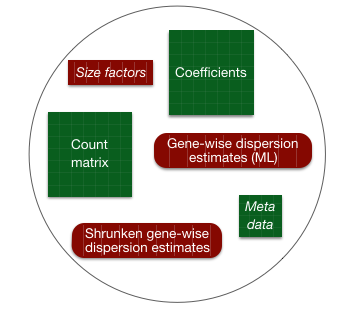
\includegraphics[keepaspectratio]{img/deseq_obj2.png}}

\section{DESeq2 differential gene expression analysis workflow}\label{deseq2-differential-gene-expression-analysis-workflow}

With these two lines of code, we have completed the core steps in the DESeq2 differential gene expression analysis. The key steps in this workflow are summarized below:

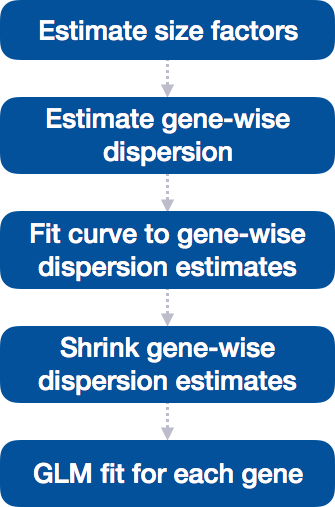
\includegraphics[width=2.08333in,height=\textheight,keepaspectratio]{img/deseq2_workflow_separate.png}

In the following sections, we will explore each step in detail to better understand how DESeq2 performs the statistical analysis and what metrics we should focus on to evaluate the quality of the results.

\subsection{Step 1: Estimate size factors}\label{step-1-estimate-size-factors}

The first step in the differential expression analysis is to estimate the size factors, which is exactly what we already did to normalize the raw counts.

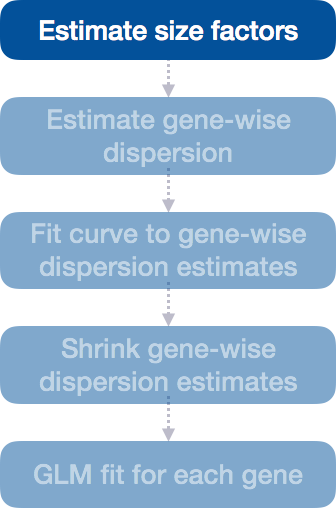
\includegraphics[width=2.08333in,height=\textheight,keepaspectratio]{img/deseq2_workflow_separate_sf.png}

DESeq2 will automatically estimate the size factors when performing the differential expression analysis. However, if you have already generated the size factors using \passthrough{\lstinline!estimateSizeFactors()!}, as we did earlier, then \passthrough{\lstinline!DESeq2!} will use these values.

To normalize the count data, \passthrough{\lstinline!DESeq2!} calculates size factors for each sample using the \emph{median of ratios method} discussed previously in the Count normalization (Chapter \ref{count-normalization}) lesson.

\subsubsection{MOV10 DE analysis: examining the size factors}\label{mov10-de-analysis-examining-the-size-factors}

Let's take a quick look at size factor values we have for each sample:

\begin{lstlisting}[language=R]
## Check the size factors
sizeFactors(dds)
\end{lstlisting}

\section{Irrel\_kd\_1 Irrel\_kd\_2 Irrel\_kd\_3 Mov10\_kd\_2 Mov10\_kd\_3 Mov10\_oe\_1 Mov10\_oe\_2}\label{irrel_kd_1-irrel_kd_2-irrel_kd_3-mov10_kd_2-mov10_kd_3-mov10_oe_1-mov10_oe_2-1}

\section{1.1224020 0.9625632 0.7477715 1.5646728 0.9351760 1.2016082 1.1205912}\label{section-2}

\section{Mov10\_oe\_3}\label{mov10_oe_3-1}

\section{0.6534987}\label{section-3}

Take a look at the total number of reads for each sample:

\begin{lstlisting}[language=R]
## Total number of raw counts per sample
colSums(counts(dds))
\end{lstlisting}

\section{Irrel\_kd\_1 Irrel\_kd\_2 Irrel\_kd\_3 Mov10\_kd\_2 Mov10\_kd\_3 Mov10\_oe\_1 Mov10\_oe\_2}\label{irrel_kd_1-irrel_kd_2-irrel_kd_3-mov10_kd_2-mov10_kd_3-mov10_oe_1-mov10_oe_2-2}

\section{22687366 19381680 14962754 32826936 19360003 23447317 21713289}\label{section-4}

\section{Mov10\_oe\_3}\label{mov10_oe_3-2}

\section{12737889}\label{section-5}

\textbf{How do the numbers correlate with the size factor?}

\begin{lstlisting}[language=R]
# Your code here
\end{lstlisting}

\subsection{Step 2: Estimate Gene-wise Dispersion}\label{step-2-estimate-gene-wise-dispersion}

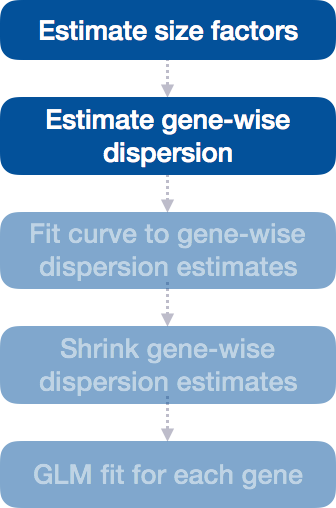
\includegraphics[width=2.08333in,height=\textheight,keepaspectratio]{img/deseq2_workflow_separate_dis.png}

The next step in differential expression analysis is estimating gene-wise dispersions. Understanding dispersion is crucial in RNA-Seq analysis.

\textbf{What is Dispersion?}

Dispersion measures the variability in gene expression that cannot be explained by the mean expression levels alone. It captures the extra-Poisson variability observed in RNA-Seq data, where the variance tends to exceed the mean due to biological and technical factors.

In DESeq2, dispersion reflects the variability in gene expression for a given mean count and is characterized by:

\begin{itemize}
\tightlist
\item
  \textbf{Lower mean counts}: Higher dispersion (more variability).
\item
  \textbf{Higher mean counts}: Lower dispersion (less variability).
\end{itemize}

The plot below illustrates the relationship between mean expression and variance: each black dot represents a gene, showing that variance can be predicted more reliably for genes with higher mean counts, while lower mean counts exhibit greater variability.

\includegraphics[width=6.25in,height=\textheight,keepaspectratio]{img/deseq_mean_vs_variance.png}

\textbf{Modeling Dispersion Using the Negative Binomial Distribution}

DESeq2 utilizes the Negative Binomial (NB) distribution to model RNA-Seq count data, effectively managing overdispersion, which is common in biological data. The two key parameters of the NB model are the mean expression level and the dispersion.

For each gene \(i\), the observed count \(Y_{ij}\) in sample \(j\) is modeled as:

\[
Y_{ij} \sim \text{NB}(\mu_{ij}, \alpha_{i})
\]

Where:
- \(Y_{ij}\) is the observed count for gene \(i\) in sample \(j\).
- \(\mu_{ij}\) is the expected normalized count for gene \(i\).
- \(\alpha_{i}\) is the gene-specific dispersion parameter.

\subsection{Step 3: Fit Curve to Gene-wise Dispersion Estimates}\label{step-3-fit-curve-to-gene-wise-dispersion-estimates}

After estimating gene-wise dispersions using maximum likelihood, DESeq2 fits a global trend to model how dispersion changes as a function of mean expression across all genes. This process stabilizes the dispersion estimates, especially for low-count genes.

\begin{itemize}
\tightlist
\item
  \textbf{Low-count genes} with more uncertain dispersion estimates are pulled closer to the global trend.
\item
  \textbf{Genes with higher counts} or more reliable estimates will be shrunk less.
\end{itemize}

\textbf{Why is Shrinkage Important?}

Shrinkage improves the reliability of dispersion estimates, making them more stable for genes with low or moderate counts, which typically have noisier estimates. This reduces the influence of random fluctuations and results in more accurate estimates for downstream differential expression testing.

Additionally, shrinkage helps to reduce false positives in differential expression analysis, ensuring that estimates for these genes are more reliable for subsequent testing.

Genes with extremely high dispersion values (outliers) may demonstrate variability that is unexpected for their mean expression levels and are typically not shrunk. These genes are often biological outliers or affected by technical issues.

\includegraphics[width=2.08333in,height=\textheight,keepaspectratio]{img/deseq2_workflow_separate_fit.png}

\subsection{Step 4: Assessing Model Fit with Dispersion Plots}\label{step-4-assessing-model-fit-with-dispersion-plots}

After shrinkage, it's essential to evaluate how well the model fits the data through dispersion plots. Ideally, most genes should scatter around the fitted curve, with dispersions decreasing as mean expression increases. Unusual patterns, such as points far from the curve, may indicate data quality issues, like outliers or contamination.

Using DESeq2's \passthrough{\lstinline!plotDispEsts()!} function visualizes the fit of the model and the extent of shrinkage across genes.

\subsubsection{Examples of Problematic Dispersion Plots}\label{examples-of-problematic-dispersion-plots}

Certainly! Problematic dispersion plots in RNA-Seq analysis, particularly when using tools like DESeq2, can arise from various issues. Here are some reasons that could lead to visual discrepancies in dispersion plots:

\textbf{Reasons for Problematic Dispersion Plots}

\begin{itemize}
\item
  \textbf{Low Count Data}:
\item
  \textbf{High Variability}: Genes with low expression levels often exhibit greater variability (higher dispersion) across replicates, leading to noisy estimates.
\item
  \textbf{Unstable Estimates}: With few counts, it's difficult to obtain reliable dispersion estimates, resulting in significant scattering in the plot.
\item
  \textbf{Outliers in the Data}:

  \begin{itemize}
  \tightlist
  \item
    \textbf{Biological Outliers}: Certain genes may genuinely exhibit high variability due to biological conditions (e.g., activation in response to stimuli), leading to higher dispersion estimates.
  \item
    \textbf{Technical Outliers}: Poor quality samples or technical errors in sequencing (e.g., contamination or failed PCR) can result in erroneous high counts for certain genes, affecting overall variability.
  \end{itemize}
\item
  \textbf{Batch Effects}:

  \begin{itemize}
  \tightlist
  \item
    Differences in sequencing runs or sample processing can introduce variability independent of biological differences. If not normalized, batch effects can distort dispersion estimates, making it seem like certain genes are more variable than they truly are.
  \end{itemize}
\item
  \textbf{Unequal Group Sizes}:

  \begin{itemize}
  \tightlist
  \item
    Uneven distribution of samples across experimental conditions can affect dispersion estimates, particularly if one group has fewer replicates or more variability.
  \end{itemize}
\item
  \textbf{Unaccounted Biological Variation}:

  \begin{itemize}
  \tightlist
  \item
    Biological variability among samples or genes that is not captured by the experimental design can affect estimates. For instance, genes involved in complex pathways may show higher dispersion due to interactions.
  \end{itemize}
\item
  \textbf{Data Quality Issues}:

  \begin{itemize}
  \tightlist
  \item
    Problems with sample handling, library construction, or sequencing can introduce discrepancies in data that visually manifest as unexpected dispersion.
  \end{itemize}
\end{itemize}

\subsection{Assessing and Addressing Issues}\label{assessing-and-addressing-issues}

To tackle issues identified in problematic dispersion plots:

\begin{itemize}
\item
  \textbf{Quality Control}: Always perform thorough quality control checks on your raw sequencing data to identify outliers and poorly performing samples.
\item
  \textbf{Filtering}: Remove low-count genes or outliers that might skew your data before running the analysis.
\item
  \textbf{Increasing Replicates}: Where possible, aim for more replicates to stabilize dispersion estimates, particularly for low-expressed genes.
\item
  \textbf{Model Evaluation}: Consider exploring different statistical models if patterns suggest that the negative binomial model is not a good fit.
\item
  \textbf{Visual Inspection}: Regularly visualize data through various methods (e.g., PCA, heatmaps, dispersion plots) to check for quality and consistency.
\end{itemize}

By understanding the potential causes for problematic dispersion plots, you can troubleshoot and improve your RNA-Seq analysis to yield more reliable results. If you have specific questions or scenarios you want to discuss, feel free to ask!

Here are examples of dispersion plots suggesting potential data quality or fitting issues:

\includegraphics[width=6.25in,height=\textheight,keepaspectratio]{img/bad_dispersion1.png}

\includegraphics[width=6.25in,height=\textheight,keepaspectratio]{img/bad_dispersion2.png}

\subsection{MOV10 Differential Expression Analysis: Exploring Dispersion Estimates}\label{mov10-differential-expression-analysis-exploring-dispersion-estimates}

Now, let's explore the dispersion estimates for the MOV10 dataset:

\begin{lstlisting}[language=R]
## Plot dispersion estimates
plotDispEsts(dds)
\end{lstlisting}

\pandocbounded{\includegraphics[keepaspectratio]{2025_RNA-Seq-Analysis_files/figure-latex/unnamed-chunk-41-1.pdf}}

\textbf{Since we have a small sample size, for many genes we see quite a bit of shrinkage. Do you think our data are a good fit for the model?}

\begin{center}\rule{0.5\linewidth}{0.5pt}\end{center}

\chapter{Negative Binomial model fitting}\label{negative-binomial-model-fitting}

\section{Generalized Linear Model fit for each gene}\label{generalized-linear-model-fit-for-each-gene}

The final step in the DESeq2 workflow is fitting the \textbf{Negative Binomial (NB) model} for each gene and performing differential expression testing. This step is crucial for identifying genes that are significantly differentially expressed between experimental conditions.

\includegraphics[width=4.16667in,height=\textheight,keepaspectratio]{img/deseq2_workflow_separate_2018.png}

DESeq2 uses a \textbf{Negative Binomial Generalized Linear Model (GLM)} to estimate the counts for each gene. A GLM is a statistical method that models relationships between variables and is an extension of linear regression. It is suitable for handling non-normally distributed data, such as RNA-seq counts, which often exhibit overdispersion (variance \textgreater{} mean).

To fit the NB GLM, DESeq2 requires two key parameters:

\begin{itemize}
\item
  \textbf{Size factor}, which accounts for differences in sequencing depth across samples.
\item
  \textbf{Dispersion estimate}, which measures variability in gene expression across replicates.
\end{itemize}

The model incorporates the estimated dispersion and the design matrix specifying the experimental conditions and covariates.

\subsection{Negative Binomial Model Formula}\label{negative-binomial-model-formula}

DESeq2 models RNA-seq counts as follows:

\[
Y_{ij} \sim \text{NB}\left(\mu_{ij}, \alpha_i\right)
\]

Where:

\begin{itemize}
\item
  \(Y_{ij}\) is the observed counts for gene \(i\) in sample \(j\)
\item
  \(\mu_{ij}\) is the expected normalized counts for gene \(i\) in sample \(j\)
\item
  \(\alpha_i\) is the dispersion parameter for gene \(i\), which has been estimated
\end{itemize}

The expected mean \(\mu_{ij}\) is modeled as:

\[
\mu_{ij} = sizeFactor_{j} \times q_{ij}
\]

Where:

\begin{itemize}
\item
  \(sizeFactor_{j}\) normalizes for differences in sequencing depth across samples
\item
  \(q_{ij}\) represents the true underlying expression level of gene \(i\) in sample \(j\), typically modeled as a function of covariates (such as experimental conditions).
\end{itemize}

\subsection{Estimating Beta Coefficients Using the Design Matrix}\label{estimating-beta-coefficients-using-the-design-matrix}

In DESeq2, \textbf{beta coefficients} (\(\beta\)) are estimated using the \textbf{design matrix}, which captures the experimental conditions for each sample (e.g., control, treatment). These coefficients represent the \textbf{log2 fold changes} in gene expression between different conditions. The estimation process involves fitting a \textbf{negative binomial generalized linear model (GLM)} to the observed count data for each gene, where the expected mean expression \(\mu_{ij}\) is modeled as a function of the design matrix \(X_j\) and the beta coefficients \(\beta_i\).

\subsection{Step-by-Step Process:}\label{step-by-step-process}

\begin{enumerate}
\def\labelenumi{\arabic{enumi}.}
\tightlist
\item
  \textbf{Define the Design Matrix \(X_j\):}
  The design matrix \(X\) includes the covariates (experimental conditions) for each sample. Each row of the matrix corresponds to a sample, and each column corresponds to a covariate (e.g., intercept, control, treatment). This matrix is generated using the \textbf{\passthrough{\lstinline!model.matrix()!}} function in R.
\end{enumerate}

\begin{lstlisting}[language=R]
X <- model.matrix(~sampletype, data = meta)

# OR

X <- model.matrix(design(dds), data = colData(dds))
\end{lstlisting}

\begin{enumerate}
\def\labelenumi{\arabic{enumi}.}
\setcounter{enumi}{1}
\tightlist
\item
  \textbf{Link Mean Expression to the Design Matrix:}
  The expected mean expression for \textbf{gene \(i\)} in \textbf{sample \(j\)} is modeled as:
\end{enumerate}

\[
\log_2(\mu_{ij}) = \beta_i X_j
\]

Or equivalently:

\[
\mu_{ij} = 2^{\beta_i X_j}
\]

Here:

\begin{itemize}
\item
  \(X_j\) is the row of the design matrix for sample \(j\) (it contains the covariates for that sample)
\item
  \(\beta_i\) is the vector of log2 fold changes (beta coefficients) for gene \(i\).
\end{itemize}

\begin{enumerate}
\def\labelenumi{\arabic{enumi}.}
\setcounter{enumi}{2}
\tightlist
\item
  \textbf{Estimate the Beta Coefficients:}
  ``DESeq2 estimates the \textbf{beta coefficients} by fitting a \textbf{negative binomial GLM} to the data using \textbf{Maximum Likelihood Estimation (MLE)}. DESeq2 substitutes the mean (\(\mu_{ij}\)) with \(2^{\beta_i X_j}\) in the negative binomial model, using MLE to predict expected counts based on experimental covariates and estimate gene expression changes while controlling for design factors.
\end{enumerate}

The model is fit using the \textbf{\passthrough{\lstinline!DESeq()!}} function in R, which carries out the entire estimation process:

\begin{lstlisting}[language=R]
dds <- DESeq(dds)
\end{lstlisting}

\begin{enumerate}
\def\labelenumi{\arabic{enumi}.}
\setcounter{enumi}{3}
\tightlist
\item
  \textbf{Extract the Beta Coefficients:}
  Once the model is fitted, the estimated beta coefficients (log2 fold changes) for each gene can be extracted using the \textbf{\passthrough{\lstinline!coef()!}} function:
\end{enumerate}

\begin{lstlisting}[language=R]
beta_coefficients <- coef(dds)
\end{lstlisting}

This gives a matrix of estimated beta coefficients, where each row corresponds to a gene and each column corresponds to a covariate in the design matrix.

\subsection{Example:}\label{example}

For example, if the design matrix includes an intercept (control) and two conditions (MOV10 knockdown and MOV10 overexpression), the beta coefficients \(\beta_i\) for gene \(i\) would represent:

\begin{itemize}
\item
  \(\beta_{i1}\): the log2 fold change for the control group (intercept)
\item
  \(\beta_{i2}\): the log2 fold change for the MOV10 knockdown group
\item
  \(\beta_{i3}\): the log2 fold change for the MOV10 overexpression group.
\end{itemize}

\subsection{Calculation:}\label{calculation}

To calculate the fitted (expected) log2 counts for \textbf{gene \(i\)} in \textbf{sample \(j\)}, you can take the \textbf{dot product} of the row of the design matrix \(X_j\) for that sample and the beta coefficients \(\beta_i\) for that gene:

\[
\log_2(\mu_{ij}) = \beta_i X_j = \beta_{i1} X_{j1} + \beta_{i2} X_{j2}  + \dots + \beta_{iP} X_{jP}
\]

Where:

\begin{itemize}
\tightlist
\item
  \(P\) is the number of covariates in the design matrix
\end{itemize}

The expected mean \(\mu_{ij}\) on the original count scale is obtained by exponentiating the log2-scale fitted values:

\[
\mu_{ij} = 2^{\beta_i X_j}
\]

\textbf{Exercise} points = +1

In the DESeq2 workflow, what is the purpose of the design matrix in the context of fitting the Negative Binomial model for each gene?

\begin{itemize}
\tightlist
\item
  Ans:
\end{itemize}

\subsection{Matrix Multiplication Form:}\label{matrix-multiplication-form}

If you want to calculate the fitted values for all genes and samples at once, you can express the model as a \textbf{matrix multiplication}:

\[
\log_2(\mu) = \beta X^T
\]

This computes the expected log2 counts for all genes across all samples.

In R, you can calculate the fitted log2 counts for all genes and samples using:

\begin{lstlisting}[language=R]
log2_fitted <- beta_coefficients %*% t(X)
\end{lstlisting}

This step multiplies the beta coefficients matrix by the transpose of the design matrix to compute the fitted log2 counts.

\subsection{\texorpdfstring{\textbf{Log2 Fold Change and Adjustments}}{Log2 Fold Change and Adjustments}}\label{log2-fold-change-and-adjustments}

The \(\beta\) coefficents are the estimates for the \textbf{log2 fold changes} for each sample group. However, \textbf{log2 fold changes} are inherently noisier when counts are low due to the large dispersion we observe with low read counts. To avoid this, the \textbf{log2 fold changes calculated by the model need to be adjusted}.

\section{Shrunken log2 foldchanges (LFC)}\label{shrunken-log2-foldchanges-lfc}

To generate more accurate LFC estimates, DESeq2 allows for the \textbf{shrinkage of the LFC estimates toward zero} when the information for a gene is low, which could include:

\begin{itemize}
\tightlist
\item
  Low counts
\item
  High dispersion values
\end{itemize}

As with the shrinkage of dispersion estimates, LFC shrinkage uses \textbf{information from all genes} to generate more accurate estimates. Specifically, the distribution of LFC estimates for all genes is used (as a prior) to shrink the LFC estimates of genes with little information or high dispersion toward more likely (lower) LFC estimates.

\includegraphics[width=5.20833in,height=\textheight,keepaspectratio]{img/deseq2_shrunken_lfc.png}

\emph{Illustration taken from the \href{https://genomebiology.biomedcentral.com/articles/10.1186/s13059-014-0550-8}{DESeq2 paper}.}

For example, in the figure above, the green gene and purple gene have the same mean values for the two sample groups (C57BL/6J and DBA/2J), but the green gene has little variation while the purple gene has high levels of variation. For the green gene with low variation, the \textbf{unshrunken LFC estimate} (vertex of the green \textbf{solid line}) is very similar to the shrunken LFC estimate (vertex of the green dotted line), but the LFC estimates for the purple gene are quite different due to the high dispersion. So even though two genes can have similar normalized count values, they can have differing degrees of LFC shrinkage. Notice the \textbf{LFC estimates are shrunken toward the prior (black solid line)}.

\textbf{Generating Shrunken LFC Estimates}
To generate the shrunken log2 fold change estimates, you have to run an additional step on your results object (that we will create below) with the function \passthrough{\lstinline!lfcShrink()!}

\subsection{Hypothesis Testing}\label{hypothesis-testing}

In DESeq2, hypothesis testing evaluates whether changes in gene expression between conditions are statistically significant. The \textbf{null hypothesis} assumes no differential expression between groups, meaning the log2 fold change is zero (\(LFC = 0\)).

\section{Statistical test for LFC estimates: Wald test}\label{statistical-test-for-lfc-estimates-wald-test}

In DESeq2, the Wald test is the default used for hypothesis testing when comparing two groups. The Wald test is a test usually performed on the LFC estimates.

DESeq2 implements the Wald test by:

\begin{itemize}
\item
  Taking the LFC and dividing it by its standard error, resulting in a z-statistic
\item
  The z-statistic is compared to a standard normal distribution, and a p-value is computed reporting the probability that a z-statistic at least as extreme as the observed value would be selected at random
\item
  If the p-value is small we reject the null hypothesis (LFC = 0) and state that there is evidence against the null (i.e.~the gene is differentially expressed).
\end{itemize}

\section{MOV10 Differential Expression Analysis: Control versus Overexpression}\label{mov10-differential-expression-analysis-control-versus-overexpression}

We have three sample classes so we can make three possible pairwise comparisons:

\begin{enumerate}
\def\labelenumi{\arabic{enumi}.}
\tightlist
\item
  Control vs.~Mov10 overexpression
\item
  Control vs.~Mov10 knockdown
\item
  Mov10 knockdown vs.~Mov10 overexpression
\end{enumerate}

\textbf{We are really only interested in \#1 and \#2 from above}. Using the design formula we provided \passthrough{\lstinline!\~ sampletype!}, indicating that this is our main factor of interest.

\subsection{Creating Contrasts for Hypothesis Testing}\label{creating-contrasts-for-hypothesis-testing}

In DESeq2, \textbf{contrasts} specify which groups to compare for differential expression testing. You can define contrasts in two ways:

\begin{enumerate}
\def\labelenumi{\arabic{enumi}.}
\item
  \textbf{Default Comparison:} DESeq2 automatically uses the alphabetically first level of the factor as the \textbf{baseline}.
\item
  \textbf{Manual Specification:} You can manually specify the comparison using the \passthrough{\lstinline!contrast!} argument in the \passthrough{\lstinline!results()!} function. The \passthrough{\lstinline!contrast!} argument takes a vector of three elements. The first element is the name of the factor (design). The second and third elements listed in the contrast are the names of the numerator and denominator level for the fold change, respectively.
\end{enumerate}

\textbf{Building the Results Table}

To build the results table, we use the \passthrough{\lstinline!results()!} function. You can specify the \passthrough{\lstinline!contrast!} to be tested using the contrast argument. In this example, we'll save the unshrunken and shrunken results of \textbf{Control vs.~Mov10 overexpression} to different variables. We'll also set the \passthrough{\lstinline!alpha!} to 0.05, which is more stringent than the default value of 0.1.

\begin{lstlisting}[language=R]
# define contrasts
contrast_oe <- c("sampletype", "MOV10_overexpression", "control")

# extract results table
res_tableOE_unshrunken <- results(dds, contrast = contrast_oe, alpha = 0.05)

resultsNames(dds)
\end{lstlisting}

\section{{[}1{]} ``Intercept''}\label{intercept}

\section{{[}2{]} ``sampletype\_MOV10\_knockdown\_vs\_control''}\label{sampletype_mov10_knockdown_vs_control}

\section{{[}3{]} ``sampletype\_MOV10\_overexpression\_vs\_control''}\label{sampletype_mov10_overexpression_vs_control}

\begin{lstlisting}[language=R]
# shrink log2 fold changes
res_tableOE <- lfcShrink(dds = dds, coef = "sampletype_MOV10_overexpression_vs_control",
    res = res_tableOE_unshrunken)

# save the results for future use
saveRDS(res_tableOE, file = "data/res_tableOE.RDS")
\end{lstlisting}

\textbf{The order of the names determines the direction of fold change that is reported.} The name provided in the second element is the level that is used as baseline. So for example, if we observe a log2 fold change of -2 this would mean the gene expression is lower in Mov10\_oe relative to the control.

\subsection{MA Plot}\label{ma-plot}

A plot that can be useful to exploring our results is the MA plot. The MA plot shows the mean of the normalized counts versus the log2 foldchanges for all genes tested. The genes that are significantly DE are colored to be easily identified. This is also a great way to illustrate the effect of LFC shrinkage. The DESeq2 package offers a simple function to generate an MA plot.

\textbf{Shrunken \& Unshrunken Results:}

\begin{lstlisting}[language=R]
par(mfrow = c(1, 2))

plotMA(res_tableOE_unshrunken, ylim = c(-2, 2))

abline(v = 10, col = "red", lwd = 2)

# Shrunken results:
plotMA(res_tableOE, ylim = c(-2, 2))

abline(v = 10, col = "red", lwd = 2)
\end{lstlisting}

\pandocbounded{\includegraphics[keepaspectratio]{2025_RNA-Seq-Analysis_files/figure-latex/unnamed-chunk-47-1.pdf}}

\textbf{MOV10 DE Analysis: Exploring the Results}

The results table in \passthrough{\lstinline!DESeq2!} looks similar to a data.frame and can be treated like one for accessing or subsetting data. However, it is stored as a \passthrough{\lstinline!DESeqResults!} object, which is important to keep in mind when working with visualization tools.

\begin{lstlisting}[language=R]
class(res_tableOE)
\end{lstlisting}

\section{{[}1{]} ``DESeqResults''}\label{deseqresults}

\section{attr(,``package'')}\label{attrpackage}

\section{{[}1{]} ``DESeq2''}\label{deseq2}

Let's go through some of the columns in the results table to get a better idea of what we are looking at. To extract information regarding the meaning of each column we can use \passthrough{\lstinline!mcols()!}:

\begin{lstlisting}[language=R]
mcols(res_tableOE, use.names = T)
\end{lstlisting}

\section{DataFrame with 5 rows and 2 columns}\label{dataframe-with-5-rows-and-2-columns}

\section{type description}\label{type-description}

\section{\texorpdfstring{ }{ }}\label{section-6}

\section{baseMean intermediate mean of normalized c..}\label{basemean-intermediate-mean-of-normalized-c..}

\section{log2FoldChange results log2 fold change (MA..}\label{log2foldchange-results-log2-fold-change-ma..}

\section{lfcSE results posterior SD: sample..}\label{lfcse-results-posterior-sd-sample..}

\section{pvalue results Wald test p-value: s..}\label{pvalue-results-wald-test-p-value-s..}

\section{padj results BH adjusted p-values}\label{padj-results-bh-adjusted-p-values}

Now let's take a look at what information is stored in the results:

\begin{lstlisting}[language=R]
head(res_tableOE)
\end{lstlisting}

\section{log2 fold change (MAP): sampletype MOV10\_overexpression vs control}\label{log2-fold-change-map-sampletype-mov10_overexpression-vs-control}

\section{Wald test p-value: sampletype MOV10 overexpression vs control}\label{wald-test-p-value-sampletype-mov10-overexpression-vs-control}

\section{DataFrame with 6 rows and 5 columns}\label{dataframe-with-6-rows-and-5-columns}

\section{baseMean log2FoldChange lfcSE pvalue padj}\label{basemean-log2foldchange-lfcse-pvalue-padj}

\section{\texorpdfstring{ }{    }}\label{section-7}

\section{1/2-SBSRNA4 45.652040 0.16820235 0.209100 0.1610752 0.2655661}\label{sbsrna4-45.652040-0.16820235-0.209100-0.1610752-0.2655661}

\section{A1BG 61.093102 0.13645896 0.176779 0.2401909 0.3603094}\label{a1bg-61.093102-0.13645896-0.176779-0.2401909-0.3603094}

\section{A1BG-AS1 175.665807 -0.04046122 0.116928 0.6789312 0.7748342}\label{a1bg-as1-175.665807--0.04046122-0.116928-0.6789312-0.7748342}

\section{A1CF 0.237692 0.00626747 0.210057 0.7945932 NA}\label{a1cf-0.237692-0.00626747-0.210057-0.7945932-na}

\section{A2LD1 89.617985 0.29017719 0.195395 0.0333343 0.0741149}\label{a2ld1-89.617985-0.29017719-0.195395-0.0333343-0.0741149}

\section{A2M 5.860084 -0.09619722 0.233561 0.1057823 0.1900466}\label{a2m-5.860084--0.09619722-0.233561-0.1057823-0.1900466}

\begin{lstlisting}[language=R]
names(res_tableOE)
\end{lstlisting}

\section{{[}1{]} ``baseMean'' ``log2FoldChange'' ``lfcSE'' ``pvalue''}\label{basemean-log2foldchange-lfcse-pvalue}

\section{{[}5{]} ``padj''}\label{padj}

\textbf{Interpreting p-values Set to NA}

In some cases, p-values or adjusted p-values may be set to NA for a gene. This happens in three scenarios:

\begin{enumerate}
\def\labelenumi{\arabic{enumi}.}
\item
  \textbf{Zero counts:} If all samples have zero counts for a gene, its baseMean will be zero, and the log2 fold change, p-value, and adjusted p-value will all be set to NA.
\item
  \textbf{Outliers:} If a gene has an extreme count outlier, its p-values will be set to NA. These outliers are detected using Cook's distance.
\item
  \textbf{Low counts:} If a gene is filtered out by independent filtering for having a low mean normalized count, only the adjusted p-value will be set to NA.
\end{enumerate}

\subsection{Multiple Testing Correction}\label{multiple-testing-correction}

When testing many genes, using raw \textbf{p-values} increases the chance of false positives (genes appearing significant by chance). If we used the \passthrough{\lstinline!p-value!} directly from the Wald test with a significance cut-off of p \textless{} 0.05, that means there is a 5\% chance it is a false positives. Each p-value is the result of a single test (single gene). The more genes we test, the more we inflate the false positive rate. This issue is the known as the \textbf{multiple testing problem.} FFor example, if we test 20,000 genes for differential expression, at p \textless{} 0.05 we would expect to find 1,000 genes by chance. If we found 3000 genes to be differentially expressed total, 150 of our genes are false positives. We would not want to sift through our ``significant'' genes to identify which ones are true positives.

DESeq2 addresses this by removing genes with low counts or outliers before testing and by applying the \textbf{Benjamini-Hochberg (BH)} method to control the \textbf{false discovery rate (FDR)}.

\subsection{Benjamini-Hochberg Adjustment}\label{benjamini-hochberg-adjustment}

The \textbf{BH-adjusted p-value} is calculated as:

\begin{enumerate}
\def\labelenumi{\arabic{enumi}.}
\item
  Sort p-values from smallest to largest.
\item
  Assign ranks to each p-value \(p_i\).
\item
  Compute the adjusted p-value:
\end{enumerate}

\[p_{i}^{adj} = p_{i} \times \frac{m}{i}\]

Where:

\begin{itemize}
\item
  \(p_{i}\) is the raw p-value
\item
  \(m\) is the total number of genes tested
\item
  \(i\) is the rank of the p-value.
\end{itemize}

\textbf{Adjusted p-values} are compared to a significance threshold (e.g., 0.05) to identify significant genes. The \textbf{Bonferroni method}, another correction, is more conservative and less commonly used due to a higher risk of false negatives.

In most cases, we should use the \textbf{adjusted p-values} (BH-corrected) to identify significant genes.

\subsection{\texorpdfstring{MOV10 DE Analysis: \textbf{Control vs.~Knockdown}}{MOV10 DE Analysis: Control vs.~Knockdown}}\label{mov10-de-analysis-control-vs.-knockdown}

After examining the overexpression results, let's move on to the comparison between \textbf{Control vs.~Knockdown}. We'll use contrasts in the \passthrough{\lstinline!results()!} function to extract the results table and store it in the \passthrough{\lstinline!res\_tableKD!} variable. You can also use \passthrough{\lstinline!coef!} to specify the contrast directly in the \passthrough{\lstinline!lfcShrink()!} function.

\begin{lstlisting}[language=R]
# define contrast
contrast_kd <- c("sampletype", "MOV10_knockdown", "control")

# extract results table
res_tableKD_unshrunken <- results(dds, contrast = contrast_kd, alpha = 0.05)

resultsNames(dds)
\end{lstlisting}

\section{{[}1{]} ``Intercept''}\label{intercept-1}

\section{{[}2{]} ``sampletype\_MOV10\_knockdown\_vs\_control''}\label{sampletype_mov10_knockdown_vs_control-1}

\section{{[}3{]} ``sampletype\_MOV10\_overexpression\_vs\_control''}\label{sampletype_mov10_overexpression_vs_control-1}

\begin{lstlisting}[language=R]
# use the `coef` argument to specify the contrast directly
res_tableKD <- lfcShrink(dds, coef = 2, res = res_tableKD_unshrunken)

## Save results for future use
saveRDS(res_tableKD, file = "data/res_tableKD.RDS")
\end{lstlisting}

\section{Summarizing Results}\label{summarizing-results}

To summarize the results, DESeq2 offers the \passthrough{\lstinline!summary()!} function, which conveniently reports the number of genes that are significantly differentially expressed at a specified threshold (\passthrough{\lstinline!default FDR < 0.05!}). Note that, even though the output refers to p-values, it actually summarizes the results using \textbf{adjusted p-values (padj/FDR)}.

Let's start by summarizing the results for the OE vs.~control comparison:

\begin{lstlisting}[language=R]
## Summarize results
summary(res_tableOE)
\end{lstlisting}

\section{}\label{section-8}

\section{out of 19748 with nonzero total read count}\label{out-of-19748-with-nonzero-total-read-count}

\section{adjusted p-value \textless{} 0.05}\label{adjusted-p-value-0.05}

\section{LFC \textgreater{} 0 (up) : 3103, 16\%}\label{lfc-0-up-3103-16}

\section{LFC \textless{} 0 (down) : 3408, 17\%}\label{lfc-0-down-3408-17}

\section{outliers {[}1{]} : 0, 0\%}\label{outliers-1-0-0}

\section{low counts {[}2{]} : 4171, 21\%}\label{low-counts-2-4171-21}

\section{(mean count \textless{} 5)}\label{mean-count-5}

\section{{[}1{]} see `cooksCutoff' argument of ?results}\label{see-cookscutoff-argument-of-results}

\section{{[}2{]} see `independentFiltering' argument of ?results}\label{see-independentfiltering-argument-of-results}

In addition to reporting the number of up- and down-regulated genes at the default significance threshold, this function also provides information on:

\begin{itemize}
\tightlist
\item
  \textbf{Number of genes tested} (genes with non-zero total read count)
\item
  \textbf{Number of genes excluded} from multiple test correction due to low mean counts
\end{itemize}

\subsection{Extracting Significant Differentially Expressed Genes}\label{extracting-significant-differentially-expressed-genes}

In some cases, using only the FDR threshold doesn't sufficiently reduce the number of significant genes, making it difficult to extract biologically meaningful results. To increase stringency, we can apply an additional fold change threshold.

Although the summary() function doesn't include an argument for fold change thresholds, we can define our own criteria.

Let's start by setting the thresholds for both adjusted p-value (FDR \textless{} 0.05) and log2 fold change (\textbar log2FC\textbar{} \textgreater{} 0.58, corresponding to a 1.5-fold change):

\begin{lstlisting}[language=R]
### Set thresholds
padj.cutoff <- 0.05
lfc.cutoff <- 0.58
\end{lstlisting}

Next, we'll convert the results table to a tibble for easier subsetting:

\begin{lstlisting}[language=R]
res_tableOE_tb <- res_tableOE %>%
    data.frame() %>%
    rownames_to_column(var = "gene") %>%
    as_tibble()
\end{lstlisting}

Now, we can filter the table to retain only the genes that meet the significance and fold change criteria:

\begin{lstlisting}[language=R]
sigOE <- res_tableOE_tb %>%
    dplyr::filter(padj < padj.cutoff & abs(log2FoldChange) > lfc.cutoff)

# Save the results for future use
saveRDS(sigOE, "data/sigOE.RDS")
\end{lstlisting}

\textbf{Exercise} points = +3

How many genes are differentially expressed in the \textbf{Overexpression vs.~Control} comparison based on the criteria we just defined? Does this reduce the number of significant genes compared to using only the FDR threshold?

\begin{lstlisting}[language=R]
# Your code here
\end{lstlisting}

\textbf{Does this reduce our results?}

\begin{lstlisting}[language=R]
# Your code here
\end{lstlisting}

\subsection{MOV10 Knockdown Analysis: Control vs.~Knockdown}\label{mov10-knockdown-analysis-control-vs.-knockdown}

Next, let's perform the same analysis for the \textbf{Control vs.~Mov10 knockdown} comparison. We'll use the same thresholds for adjusted p-value (FDR \textless{} 0.05) and log2 fold change (\textbar log2FC\textbar{} \textgreater{} 0.58).

\begin{lstlisting}[language=R]
res_tableKD_tb <- res_tableKD %>%
    data.frame() %>%
    rownames_to_column(var = "gene") %>%
    as_tibble()

sigKD <- res_tableKD_tb %>%
    dplyr::filter(padj < padj.cutoff & abs(log2FoldChange) > lfc.cutoff)

# We'll save this object for use in the homework
saveRDS(sigKD, "data/sigKD.RDS")
\end{lstlisting}

\textbf{How many genes are differentially expressed in the Knockdown compared to Control?}

\begin{lstlisting}[language=R]
# Your code here
\end{lstlisting}

With our subset of significant genes identified, we can now proceed to visualize the results and explore patterns of differential expression.

\begin{lstlisting}[language=R]
## Save all objects for later
save.image()
\end{lstlisting}

\chapter{Visualizing RNA-seq results}\label{visualizing-rna-seq-results}

During this lesson, we will get you started with some basic and more advanced visualization techniques to explore and interpret the results of your differential expression analysis.

Let's start by loading a few libraries:

\begin{lstlisting}[language=R]
# load libraries
library(tidyverse)
library(ggplot2)
library(ggrepel)
library(RColorBrewer)
library(DESeq2)
library(pheatmap)
library(dplyr)
\end{lstlisting}

We will be working with three different data objects we have already created in earlier lessons:

\begin{itemize}
\tightlist
\item
  Metadata for our samples (a dataframe): \passthrough{\lstinline!meta!}
\item
  Normalized expression data for every gene in each of our samples (a matrix): \passthrough{\lstinline!normalized\_counts!}
\item
  Tibble versions of the DESeq2 results we generated in the last lesson: \passthrough{\lstinline!res\_tableOE\_tb!} and \passthrough{\lstinline!res\_tableKD\_tb!}
\end{itemize}

Let's create tibble objects from the \passthrough{\lstinline!meta!} and \passthrough{\lstinline!normalized\_counts!} data frames before we start plotting. This will enable us to use the \passthrough{\lstinline!tidyverse!} functionality more easily.

Check to make sure the column names of the \passthrough{\lstinline!normalized\_counts!} matrix are the same as the row names of the \passthrough{\lstinline!meta!} data frame. If they are not, you will need to reorder the columns of \passthrough{\lstinline!normalized\_counts!} to match the row names of \passthrough{\lstinline!meta!}.

\begin{lstlisting}[language=R]
# Read in the metadata
meta <- read.table("data/Mov10_full_meta.txt", header = T, row.names = 1)

# Create a tibble for meta data
mov10_meta <- meta %>%
    rownames_to_column(var = "samplename") %>%
    as_tibble()

# read in the normalized counts
normalized_counts <- read.delim("data/normalized_counts.txt", row.names = 1)

all(mov10_meta$samplename == colnames(normalized_counts))
\end{lstlisting}

\section{{[}1{]} TRUE}\label{true-2}

\begin{lstlisting}[language=R]
# Create a tibble for normalized_counts
normalized_counts <- normalized_counts %>%
    data.frame() %>%
    rownames_to_column(var = "gene") %>%
    as_tibble()
\end{lstlisting}

\subsection{Plotting signicant DE genes}\label{plotting-signicant-de-genes}

One way to visualize results would be to simply plot the expression data for a handful of genes. We could do that by picking out specific genes of interest or selecting a range of genes.

\subsubsection{\texorpdfstring{\textbf{Using DESeq2 \texttt{plotCounts()} to plot expression of a single gene}}{Using DESeq2 plotCounts() to plot expression of a single gene}}\label{using-deseq2-plotcounts-to-plot-expression-of-a-single-gene}

To pick out a specific gene of interest to plot, for example Mov10, we can use the \passthrough{\lstinline!plotCounts()!} from DESeq2. \passthrough{\lstinline!plotCounts()!} is a function that allows us to plot the normalized counts for a single gene across all samples.

\begin{lstlisting}[language=R]
plotCounts(dds, gene = "MOV10", intgroup = "sampletype")
\end{lstlisting}

\pandocbounded{\includegraphics[keepaspectratio]{2025_RNA-Seq-Analysis_files/figure-latex/unnamed-chunk-63-1.pdf}}

\begin{lstlisting}[language=R]
# We can also color the points by sample type
sampletype = as.factor(mov10_meta$sampletype)

library(RColorBrewer)

display.brewer.all()
\end{lstlisting}

\pandocbounded{\includegraphics[keepaspectratio]{2025_RNA-Seq-Analysis_files/figure-latex/unnamed-chunk-63-2.pdf}}

\begin{lstlisting}[language=R]
col = brewer.pal(8, "Dark2")
palette(col)

plotCounts(dds, gene = "MOV10", intgroup = "sampletype", col = as.numeric(sampletype),
    pch = 19)
\end{lstlisting}

\pandocbounded{\includegraphics[keepaspectratio]{2025_RNA-Seq-Analysis_files/figure-latex/unnamed-chunk-63-3.pdf}}

\textbf{This function only allows for plotting the counts of a single gene at a time.}

\subsubsection{\texorpdfstring{\textbf{Using ggplot2 to plot expression of a single gene}}{Using ggplot2 to plot expression of a single gene}}\label{using-ggplot2-to-plot-expression-of-a-single-gene}

We can also use ggplot2 to plot the \passthrough{\lstinline!MOV10!} counts. We can save the output of \passthrough{\lstinline!plotCounts()!} to a variable specifying the \passthrough{\lstinline!returnData=TRUE!} argument. This will save the normalized counts for the gene \passthrough{\lstinline!MOV10!} to a data frame object. We can then use ggplot2 to plot the normalized counts for \passthrough{\lstinline!MOV10!} across all samples.

\begin{lstlisting}[language=R]
# Save `plotCounts()` to a data frame object
d <- plotCounts(dds, gene = "MOV10", intgroup = "sampletype", returnData = TRUE)

# Plot using ggplot2
ggplot(d, aes(x = sampletype, y = count, color = sampletype)) + geom_point(position = position_jitter(w = 0.1,
    h = 0)) + geom_text_repel(aes(label = rownames(d))) + theme_bw() + ggtitle("MOV10") +
    theme(plot.title = element_text(hjust = 0.5))
\end{lstlisting}

\pandocbounded{\includegraphics[keepaspectratio]{2025_RNA-Seq-Analysis_files/figure-latex/unnamed-chunk-64-1.pdf}}

\begin{quote}
Note that in the plot below (code above), we are using \passthrough{\lstinline!geom\_text\_repel()!} from the \passthrough{\lstinline!ggrepel!} package to label our individual points on the plot.
\end{quote}

\subsubsection{\texorpdfstring{Using \texttt{ggplot2} to plot multiple genes (e.g.~top 20)}{Using ggplot2 to plot multiple genes (e.g.~top 20)}}\label{using-ggplot2-to-plot-multiple-genes-e.g.-top-20}

Often it is helpful to check the expression of multiple genes of interest at the same time. This often first requires some data wrangling.

We are going to plot the normalized count values for the \textbf{top 20 differentially expressed genes (by padj values)}.

To do this, we first need to determine the gene names of our top 20 genes by ordering our results and extracting the top 20 genes (by padj values):

\begin{lstlisting}[language=R]
res_tableOE <- readRDS("data/res_tableOE.RDS")

res_tableOE_tb <- res_tableOE %>%
    data.frame() %>%
    rownames_to_column(var = "gene") %>%
    as_tibble()

## Order results by padj values
top20_sigOE_genes <- res_tableOE_tb %>%
    arrange(padj) %>%
    # Arrange rows by padj values
pull(gene) %>%
    # Extract character vector of ordered genes
head(n = 20)
# Extract the first 20 genes
\end{lstlisting}

Then, we can extract the normalized count values for these top 20 genes:

\begin{lstlisting}[language=R]
## Normalized counts for top 20 significant genes
top20_sigOE_norm <- normalized_counts %>%
    filter(gene %in% top20_sigOE_genes)
\end{lstlisting}

Now that we have the normalized counts for each of the top 20 genes for all 8 samples, to plot using \passthrough{\lstinline!ggplot()!}, we need to \passthrough{\lstinline!pivot\_longer!} top20\_sigOE\_norm from a wide format to a long format so the counts for all samples will be in a single column to allow us to give ggplot the one column with the values we want it to plot.

The \passthrough{\lstinline!pivot\_longer()!} function in the \textbf{tidyr} package will perform this operation and will output the normalized counts for all genes for \emph{Mov10\_oe\_1} listed in the first 20 rows, followed by the normalized counts for \emph{Mov10\_oe\_2} in the next 20 rows, so on and so forth.

\includegraphics[width=8.33333in,height=\textheight,keepaspectratio]{img/melt_wide_to_long_format.png}

\begin{lstlisting}[language=R]
# Pivot the data frame
pivoted_top20_sigOE <- top20_sigOE_norm %>%
    pivot_longer(colnames(top20_sigOE_norm)[2:9], names_to = "samplename", values_to = "normalized_counts")

## Check the column header in the 'pivoted' data frame
head(pivoted_top20_sigOE)
\end{lstlisting}

\section{\# A tibble: 6 x 3}\label{a-tibble-6-x-3}

\section{gene samplename normalized\_counts}\label{gene-samplename-normalized_counts}

\section{\texorpdfstring{ }{  }}\label{section-9}

\section{1 ADAMTS1 Irrel\_kd\_1 6718.}\label{adamts1-irrel_kd_1-6718.}

\section{2 ADAMTS1 Irrel\_kd\_2 6455.}\label{adamts1-irrel_kd_2-6455.}

\section{3 ADAMTS1 Irrel\_kd\_3 6802.}\label{adamts1-irrel_kd_3-6802.}

\section{4 ADAMTS1 Mov10\_kd\_2 6869.}\label{adamts1-mov10_kd_2-6869.}

\section{5 ADAMTS1 Mov10\_kd\_3 8731.}\label{adamts1-mov10_kd_3-8731.}

\section{6 ADAMTS1 Mov10\_oe\_1 13252.}\label{adamts1-mov10_oe_1-13252.}

Now, if we want our counts colored by sample group, then we need to combine the metadata information with the melted normalized counts data into the same data frame for input to \passthrough{\lstinline!ggplot()!}:

\passthrough{\lstinline!inner\_join(x,y)!} will merge 2 data frames by the colname in x that matches a column name in y in this case \passthrough{\lstinline!samplename!} column.

\begin{lstlisting}[language=R]
pivoted_top20_sigOE <- inner_join(mov10_meta, pivoted_top20_sigOE)
\end{lstlisting}

Now that we have a data frame in a format that can be utilised by ggplot easily, let's plot!

\begin{lstlisting}[language=R]
## plot using ggplot2
ggplot(pivoted_top20_sigOE) + geom_point(aes(x = gene, y = normalized_counts, color = sampletype)) +
    scale_y_log10() + xlab("Genes") + ylab("log10 Normalized Counts") + ggtitle("Top 20 Significant DE Genes") +
    theme_bw() + theme(axis.text.x = element_text(angle = 45, hjust = 1)) + theme(plot.title = element_text(hjust = 0.5))
\end{lstlisting}

\pandocbounded{\includegraphics[keepaspectratio]{2025_RNA-Seq-Analysis_files/figure-latex/unnamed-chunk-69-1.pdf}}

\subsection{Heatmap}\label{heatmap}

We will plot a heatmap of the \passthrough{\lstinline!sigOE!} genes to visualize their expression across all samples using \passthrough{\lstinline!pheatmap()!}.

\begin{lstlisting}[language=R]
sigOE = readRDS("data/sigOE.RDS")

norm_OEsig <- normalized_counts[, c(1, 2:4, 7:9)] %>%
    filter(gene %in% sigOE$gene) %>%
    data.frame() %>%
    column_to_rownames(var = "gene")
\end{lstlisting}

Now let's draw the heatmap using pheatmap. We can also add annotations to the heatmap to indicate the sample type. The \passthrough{\lstinline!annotation\_col!} argument in \passthrough{\lstinline!pheatmap()!}requires a data frame with the same row names as the column names of the matrix used to generate the heatmap.

\begin{lstlisting}[language=R]
### Annotate our heatmap (optional)
annotation <- mov10_meta %>%
    filter(samplename %in% colnames(norm_OEsig)) %>%
    dplyr::select(samplename, sampletype) %>%
    data.frame(row.names = "samplename")

annotation$sampletype = factor(annotation$sampletype)

### Set a color palette
heat_colors <- brewer.pal(6, "YlOrRd")

### Set annotation colors
ann_colors = list(sampletype = c(control = "navy", MOV10_overexpression = "green"))

### Run pheatmap
pheatmap(norm_OEsig, annotation_colors = ann_colors, color = heat_colors, cluster_rows = T,
    show_rownames = F, annotation_col = annotation, border_color = NA, fontsize = 12,
    scale = "row", fontsize_col = 12)
\end{lstlisting}

\pandocbounded{\includegraphics[keepaspectratio]{2025_RNA-Seq-Analysis_files/figure-latex/unnamed-chunk-71-1.pdf}}

\begin{quote}
\emph{NOTE:} There are several additional arguments we have included in the function for aesthetics. One important one is \passthrough{\lstinline!scale="row"!}, in which Z-scores are plotted, rather than the actual normalized count value.
\end{quote}

\subsection{Volcano plots}\label{volcano-plots}

A commonly used plot in RNA-seq analysis is the \textbf{volcano plot}. in which you have the log transformed adjusted p-values plotted on the y-axis and log2 fold change values on the x-axis.

To generate a volcano plot, we first need to have a column in our results data indicating whether or not the gene is considered differentially expressed based on p-adjusted values.

\begin{lstlisting}[language=R]
## create a column for thresholding in the results table
res_tableOE_tb <- res_tableOE_tb %>%
    mutate(threshold_OE = padj < 0.05 & abs(log2FoldChange) >= 0.58)
\end{lstlisting}

Now we can start plotting. The \passthrough{\lstinline!geom\_point!} object is most applicable, as this is essentially a scatter plot:

\begin{lstlisting}[language=R]
ggplot(res_tableOE_tb) + geom_point(aes(x = log2FoldChange, y = -log10(padj), colour = threshold_OE)) +
    ggtitle("Mov10 overexpression") + xlab("log2 fold change") + ylab("-log10 adjusted p-value") +
    theme_bw() + theme(legend.position = "none", plot.title = element_text(size = rel(1.5),
    hjust = 0.5), axis.title = element_text(size = rel(1.25)))
\end{lstlisting}

\pandocbounded{\includegraphics[keepaspectratio]{2025_RNA-Seq-Analysis_files/figure-latex/unnamed-chunk-73-1.pdf}}

What if we also wanted to know where the top 10 genes (lowest padj) in our DE list are located on this plot? We could label those dots with the gene name on the volcano plot using \passthrough{\lstinline!geom\_text\_repel()!}.

First, we need to order the res\_tableOE tibble by \passthrough{\lstinline!padj!}, and add an additional column to it, to include on those gene names we want to use to label the plot.

\begin{lstlisting}[language=R]
## Create a column to indicate which genes to label
res_tableOE_tb <- res_tableOE_tb %>%
    arrange(padj) %>%
    mutate(genelabels = "")

res_tableOE_tb$genelabels[1:10] <- res_tableOE_tb$gene[1:10]

head(res_tableOE_tb)
\end{lstlisting}

\section{\# A tibble: 6 x 8}\label{a-tibble-6-x-8}

\section{gene baseMean log2FoldChange lfcSE pvalue padj threshold\_OE}\label{gene-basemean-log2foldchange-lfcse-pvalue-padj-threshold_oe}

\section{\texorpdfstring{ }{      }}\label{section-10}

\section{1 MOV10 21682. 5.08 0.110 0 0 TRUE}\label{mov10-21682.-5.08-0.110-0-0-true}

\section{2 H1F0 7881. 1.55 0.0566 3.00e-166 2.34e-162 TRUE}\label{h1f0-7881.-1.55-0.0566-3.00e-166-2.34e-162-true}

\section{3 HIST1H1C 1741. 1.52 0.0706 2.06e-104 1.07e-100 TRUE}\label{hist1h1c-1741.-1.52-0.0706-2.06e-104-1.07e-100-true}

\section{4 TXNIP 5134. 1.42 0.0697 1.62e- 93 6.33e- 90 TRUE}\label{txnip-5134.-1.42-0.0697-1.62e--93-6.33e--90-true}

\section{5 NEAT1 21974. 0.916 0.0467 8.28e- 87 2.58e- 83 TRUE}\label{neat1-21974.-0.916-0.0467-8.28e--87-2.58e--83-true}

\section{6 KLF10 1694. 1.23 0.0652 4.77e- 81 1.24e- 77 TRUE}\label{klf10-1694.-1.23-0.0652-4.77e--81-1.24e--77-true}

\section{\texorpdfstring{\# i 1 more variable: genelabels }{\# i 1 more variable: genelabels }}\label{i-1-more-variable-genelabels}

Next, we plot it as before with an additiona layer for \passthrough{\lstinline!geom\_text\_repel()!} wherein we can specify the column of gene labels we just created.

\begin{lstlisting}[language=R]
ggplot(res_tableOE_tb, aes(x = log2FoldChange, y = -log10(padj))) + geom_point(aes(colour = threshold_OE)) +
    geom_text_repel(aes(label = genelabels)) + ggtitle("Mov10 overexpression") +
    xlab("log2 fold change") + ylab("-log10 adjusted p-value") + theme_bw() + theme(legend.position = "none",
    plot.title = element_text(size = rel(1.5), hjust = 0.5), axis.title = element_text(size = rel(1.25)))
\end{lstlisting}

\pandocbounded{\includegraphics[keepaspectratio]{2025_RNA-Seq-Analysis_files/figure-latex/unnamed-chunk-75-1.pdf}}

\begin{center}\rule{0.5\linewidth}{0.5pt}\end{center}

\chapter{Summary of DGE workflow}\label{summary-of-dge-workflow}

\textbf{Homework: modify this file to analyze the MOV dataset, starting with Mov10\_full\_counts.txt in your data folder. Compare the ``MOV10\_knockdown'' to the ``control''. Include a heatmap and a volcano plot} points = +10

\begin{lstlisting}[language=R]
## Setup
library(DESeq2)
\end{lstlisting}

We have detailed the various steps in a differential expression analysis workflow, providing theory with example code. To provide a more succinct reference for the code needed to run a DGE analysis, we have summarized the steps in an analysis below:

\subsection{1. Import data into dds object:}\label{import-data-into-dds-object}

\begin{lstlisting}[language=R]
# Check that the row names of the metadata equal the column names of the **raw
# counts** data
all(colnames(raw_counts) == rownames(metadata))

# Create DESeq2Dataset object
dds <- DESeqDataSetFromMatrix(countData = raw_counts, colData = metadata, design = ~condition)
\end{lstlisting}

\subsection{2. Exploratory data analysis (PCA \& heirarchical clustering) - identifying outliers and sources of variation in the data:}\label{exploratory-data-analysis-pca-heirarchical-clustering---identifying-outliers-and-sources-of-variation-in-the-data}

\begin{lstlisting}[language=R]
# Transform counts for data visualization
rld <- rlog(dds, blind = TRUE)

# Plot PCA
plotPCA(rld, intgroup = "sampletype")

# Extract the rlog matrix from the object
rld_mat <- assay(rld)

# Compute pairwise correlation values
rld_cor <- cor(rld_mat)

# Plot heatmap
pheatmap(rld_cor)
\end{lstlisting}

\subsection{3. Run DESeq2:}\label{run-deseq2}

\begin{lstlisting}[language=R]
# **Optional step** - Re-create DESeq2 dataset if the design formula has
# changed after QC analysis in include other sources of variation

dds <- DESeqDataSetFromMatrix(countData = raw_counts, colData = metadata, design = ~condition)

# Run DESeq2 differential expression analysis
dds <- DESeq(dds)

# Output normalized counts to save as a file to access outside RStudio
normalized_counts <- counts(dds, normalized = TRUE)

write.table(normalized_counts, file = "data/normalized_counts.txt", sep = "\t", quote = F,
    col.names = NA)
\end{lstlisting}

\subsection{4. Check the fit of the dispersion estimates:}\label{check-the-fit-of-the-dispersion-estimates}

\begin{lstlisting}[language=R]
# Plot dispersion estimates
plotDispEsts(dds)
\end{lstlisting}

\subsection{5. Create contrasts to perform Wald testing on the shrunken log2 foldchanges between specific conditions:}\label{create-contrasts-to-perform-wald-testing-on-the-shrunken-log2-foldchanges-between-specific-conditions}

\begin{lstlisting}[language=R]
# Output results of Wald test for contrast
contrast <- c("condition", "level_to_compare", "base_level")

res <- results(dds, contrast = contrast)

coef = resultsNames(dds)

res_table <- lfcShrink(dds, coef = coef[2], res = res, type = "apeglm")
\end{lstlisting}

\subsection{6. Output significant results:}\label{output-significant-results}

\begin{lstlisting}[language=R]
### Set thresholds
padj.cutoff <- 0.05
lfc.cutoff <- 0.58  ## change in expression of 1.5

# Turn the results object into a data frame
res_df <- res %>%
    data.frame() %>%
    rownames_to_column(var = "gene")

# Subset the significant results
sig_res <- dplyr::filter(res_df, padj < padj.cutoff & abs(log2FoldChange) > lfc.cutoff)
\end{lstlisting}

\subsection{7. Visualize results: volcano plots, heatmaps, normalized counts plots of top genes, etc.}\label{visualize-results-volcano-plots-heatmaps-normalized-counts-plots-of-top-genes-etc.}

\subsection{8. Make sure to output the versions of all tools used in the DE analysis:}\label{make-sure-to-output-the-versions-of-all-tools-used-in-the-de-analysis}

\begin{lstlisting}[language=R]
sessionInfo()
\end{lstlisting}

\section{R version 4.5.1 (2025-06-13)}\label{r-version-4.5.1-2025-06-13}

\section{Platform: x86\_64-apple-darwin20}\label{platform-x86_64-apple-darwin20}

\section{Running under: macOS Sequoia 15.6}\label{running-under-macos-sequoia-15.6}

\section{}\label{section-11}

\section{Matrix products: default}\label{matrix-products-default}

\section{BLAS: /Library/Frameworks/R.framework/Versions/4.5-x86\_64/Resources/lib/libRblas.0.dylib}\label{blas-libraryframeworksr.frameworkversions4.5-x86_64resourcesliblibrblas.0.dylib}

\section{LAPACK: /Library/Frameworks/R.framework/Versions/4.5-x86\_64/Resources/lib/libRlapack.dylib; LAPACK version 3.12.1}\label{lapack-libraryframeworksr.frameworkversions4.5-x86_64resourcesliblibrlapack.dylib-lapack-version-3.12.1}

\section{}\label{section-12}

\section{locale:}\label{locale}

\section{{[}1{]} en\_CA.UTF-8/en\_CA.UTF-8/en\_CA.UTF-8/C/en\_CA.UTF-8/en\_CA.UTF-8}\label{en_ca.utf-8en_ca.utf-8en_ca.utf-8cen_ca.utf-8en_ca.utf-8}

\section{}\label{section-13}

\section{time zone: America/Los\_Angeles}\label{time-zone-americalos_angeles}

\section{tzcode source: internal}\label{tzcode-source-internal}

\section{}\label{section-14}

\section{attached base packages:}\label{attached-base-packages}

\section{{[}1{]} stats4 stats graphics grDevices utils datasets methods}\label{stats4-stats-graphics-grdevices-utils-datasets-methods}

\section{{[}8{]} base}\label{base}

\section{}\label{section-15}

\section{other attached packages:}\label{other-attached-packages}

\section{{[}1{]} ggrepel\_0.9.6 pheatmap\_1.0.13}\label{ggrepel_0.9.6-pheatmap_1.0.13}

\section{{[}3{]} DESeq2\_1.48.1 SummarizedExperiment\_1.38.1}\label{deseq2_1.48.1-summarizedexperiment_1.38.1}

\section{{[}5{]} Biobase\_2.68.0 MatrixGenerics\_1.20.0}\label{biobase_2.68.0-matrixgenerics_1.20.0}

\section{{[}7{]} matrixStats\_1.5.0 GenomicRanges\_1.60.0}\label{matrixstats_1.5.0-genomicranges_1.60.0}

\section{{[}9{]} GenomeInfoDb\_1.44.1 IRanges\_2.42.0}\label{genomeinfodb_1.44.1-iranges_2.42.0}

\section{{[}11{]} S4Vectors\_0.46.0 BiocGenerics\_0.54.0}\label{s4vectors_0.46.0-biocgenerics_0.54.0}

\section{{[}13{]} generics\_0.1.4 RColorBrewer\_1.1-3}\label{generics_0.1.4-rcolorbrewer_1.1-3}

\section{{[}15{]} lubridate\_1.9.4 forcats\_1.0.0}\label{lubridate_1.9.4-forcats_1.0.0}

\section{{[}17{]} stringr\_1.5.1 dplyr\_1.1.4}\label{stringr_1.5.1-dplyr_1.1.4}

\section{{[}19{]} purrr\_1.1.0 readr\_2.1.5}\label{purrr_1.1.0-readr_2.1.5}

\section{{[}21{]} tidyr\_1.3.1 tibble\_3.3.0}\label{tidyr_1.3.1-tibble_3.3.0}

\section{{[}23{]} ggplot2\_3.5.2 tidyverse\_2.0.0}\label{ggplot2_3.5.2-tidyverse_2.0.0}

\section{}\label{section-16}

\section{loaded via a namespace (and not attached):}\label{loaded-via-a-namespace-and-not-attached}

\section{{[}1{]} gtable\_0.3.6 xfun\_0.52 lattice\_0.22-7}\label{gtable_0.3.6-xfun_0.52-lattice_0.22-7}

\section{{[}4{]} numDeriv\_2016.8-1.1 tzdb\_0.5.0 vctrs\_0.6.5}\label{numderiv_2016.8-1.1-tzdb_0.5.0-vctrs_0.6.5}

\section{{[}7{]} tools\_4.5.1 parallel\_4.5.1 fansi\_1.0.6}\label{tools_4.5.1-parallel_4.5.1-fansi_1.0.6}

\section{{[}10{]} pkgconfig\_2.0.3 Matrix\_1.7-3 lifecycle\_1.0.4}\label{pkgconfig_2.0.3-matrix_1.7-3-lifecycle_1.0.4}

\section{{[}13{]} GenomeInfoDbData\_1.2.14 compiler\_4.5.1 farver\_2.1.2}\label{genomeinfodbdata_1.2.14-compiler_4.5.1-farver_2.1.2}

\section{{[}16{]} codetools\_0.2-20 htmltools\_0.5.8.1 yaml\_2.3.10}\label{codetools_0.2-20-htmltools_0.5.8.1-yaml_2.3.10}

\section{{[}19{]} pillar\_1.11.0 crayon\_1.5.3 MASS\_7.3-65}\label{pillar_1.11.0-crayon_1.5.3-mass_7.3-65}

\section{{[}22{]} BiocParallel\_1.42.1 DelayedArray\_0.34.1 emdbook\_1.3.14}\label{biocparallel_1.42.1-delayedarray_0.34.1-emdbook_1.3.14}

\section{{[}25{]} abind\_1.4-8 bdsmatrix\_1.3-7 tidyselect\_1.2.1}\label{abind_1.4-8-bdsmatrix_1.3-7-tidyselect_1.2.1}

\section{{[}28{]} locfit\_1.5-9.12 digest\_0.6.37 mvtnorm\_1.3-3}\label{locfit_1.5-9.12-digest_0.6.37-mvtnorm_1.3-3}

\section{{[}31{]} stringi\_1.8.7 bookdown\_0.43 labeling\_0.4.3}\label{stringi_1.8.7-bookdown_0.43-labeling_0.4.3}

\section{{[}34{]} fastmap\_1.2.0 grid\_4.5.1 cli\_3.6.5}\label{fastmap_1.2.0-grid_4.5.1-cli_3.6.5}

\section{{[}37{]} SparseArray\_1.8.1 magrittr\_2.0.3 S4Arrays\_1.8.1}\label{sparsearray_1.8.1-magrittr_2.0.3-s4arrays_1.8.1}

\section{{[}40{]} utf8\_1.2.6 withr\_3.0.2 scales\_1.4.0}\label{utf8_1.2.6-withr_3.0.2-scales_1.4.0}

\section{{[}43{]} UCSC.utils\_1.4.0 timechange\_0.3.0 rmarkdown\_2.29}\label{ucsc.utils_1.4.0-timechange_0.3.0-rmarkdown_2.29}

\section{{[}46{]} XVector\_0.48.0 httr\_1.4.7 hms\_1.1.3}\label{xvector_0.48.0-httr_1.4.7-hms_1.1.3}

\section{{[}49{]} coda\_0.19-4.1 evaluate\_1.0.4 knitr\_1.50}\label{coda_0.19-4.1-evaluate_1.0.4-knitr_1.50}

\section{{[}52{]} bbmle\_1.0.25.1 rlang\_1.1.6 Rcpp\_1.1.0}\label{bbmle_1.0.25.1-rlang_1.1.6-rcpp_1.1.0}

\section{{[}55{]} glue\_1.8.0 formatR\_1.14 apeglm\_1.30.0}\label{glue_1.8.0-formatr_1.14-apeglm_1.30.0}

\section{{[}58{]} rstudioapi\_0.17.1 jsonlite\_2.0.0 plyr\_1.8.9}\label{rstudioapi_0.17.1-jsonlite_2.0.0-plyr_1.8.9}

\section{{[}61{]} R6\_2.6.1}\label{r6_2.6.1}

\chapter{Functional analysis of RNAseq data}\label{functional-analysis-of-rnaseq-data}

\subsection{Ontology and GO Terms}\label{ontology-and-go-terms}

\textbf{Ontology}:
An ontology is a representation of something we know about. Ontologies consist of representations of things that are detectable or directly observable and the relationships between those things.
The \textbf{Gene Ontology (GO)} project provides an ontology of defined terms representing gene product properties. These terms are connected to each other via formally defined relationships, allowing for consistent annotation and analysis of gene functions across different species and research areas.

\subsection{GO Terms (Gene Ontology Terms)}\label{go-terms-gene-ontology-terms}

The GO terms describe three aspects of gene products:

\begin{itemize}
\tightlist
\item
  \textbf{Biological Process}: Refers to the biological objectives achieved by gene products, such as ``cell division'' or ``response to stress.''
\end{itemize}

\pandocbounded{\includegraphics[keepaspectratio]{img/go_heirarchy.jpg}}

\begin{itemize}
\item
  \textbf{Molecular Function}: Describes the biochemical activities at the molecular level, such as ``enzyme activity'' or ``DNA binding.''
\item
  \textbf{Cellular Component}: Indicates where gene products are located within the cell, like ``nucleus'' or ``mitochondrion.''
\end{itemize}

\subsection{GO Enrichment Methods}\label{go-enrichment-methods}

\pandocbounded{\includegraphics[keepaspectratio]{img/pathway_analysis.png}}

GO enrichment methods help interpret differentially expressed gene lists from RNA-Seq data and include the following:

\begin{enumerate}
\def\labelenumi{\arabic{enumi}.}
\tightlist
\item
  \textbf{Overrepresentation Analysis (ORA)}:
\end{enumerate}

\begin{itemize}
\tightlist
\item
  ORA assesses whether specific GO terms are over-represented in a gene list compared to the background set of genes (e.g., all genes in the genome). Over-represented GO terms indicate biological functions or processes that are significantly associated with the genes of interest.
\end{itemize}

\includegraphics[width=6.25in,height=\textheight,keepaspectratio]{img/go_proportions.png}

\includegraphics[width=6.25in,height=\textheight,keepaspectratio]{img/go_proportions_table3.png}`

\begin{itemize}
\tightlist
\item
  \textbf{Hypergeometric Test}:
  The hypergeometric test in GO enrichment analysis is used to determine whether a set of genes is enriched for specific GO terms compared to the background set of genes. The test calculates the probability of observing the overlap between the query gene set and the gene set associated with a particular GO term, given the total number of genes in the dataset and the number of genes in the background set.
\end{itemize}

The formula for the cumulative probability of observing \textbf{at most \(q\)} successes (the lower-tail probability) in a sample of size \(k\) from a population with \(m\) successes and \(N - m\) failures is:
\[
P(X \leq q) = \sum_{i=0}^{q} \frac{\binom{m}{i} \binom{N - m}{k - i}}{\binom{N}{k}}
\]
Where:

\textbf{\passthrough{\lstinline!q!}}: The \textbf{number of genes in your list of interest that are annotated with a specific GO term} (e.g., genes in your differential expression results that are associated with ``cell cycle regulation'').

\textbf{\passthrough{\lstinline!m!}}: The \textbf{total number of genes in the background set (e.g., all genes in the genome) that are annotated with the specific GO term} (e.g., all genes associated with ``cell cycle regulation'' in the entire dataset or genome).

\textbf{\passthrough{\lstinline!N!}}: The \textbf{total number of genes in the background set.}

\textbf{\passthrough{\lstinline!k!}}: The \textbf{total number of genes in your gene list of interest}

\subsection{Example}\label{example-1}

Suppose:your background population has \(N = 20,000\) genes (e.g., the entire genome). Out of these, \(m = 500\) genes are associated with a specific GO term (e.g., ``cell cycle regulation''). You have a list of \(k = 1000\) genes of interest. In this list, \(q = 30\) genes are associated with the ``cell cycle regulation'' GO term.

\begin{lstlisting}[language=R]
# Define parameters
N <- 20000  # Total genes in the background (population)
m <- 500  # Total genes associated with the GO term in the background
k <- 1000  # Sample size (genes in your list)
q <- 50  # Observed number of successes (overlap with GO term)

# Perform the hypergeometric test (upper-tail probability)
p_value <- phyper(q - 1, m, N - m, k, lower.tail = FALSE)
p_value
\end{lstlisting}

\section{{[}1{]} 2.551199e-06}\label{e-06}

\begin{enumerate}
\def\labelenumi{\arabic{enumi}.}
\setcounter{enumi}{1}
\tightlist
\item
  \textbf{Gene Set Enrichment Analysis (GSEA)}:
  Instead of only considering genes above a certain threshold (e.g., differentially expressed genes), GSEA looks at the \textbf{entire ranked list of genes} (e.g., ranked by their expression levels) and checks whether genes associated with a certain GO term are \emph{statistically over-represented at the top or bottom of a ranked gene list, indicating coordinated changes in gene expression}.
\end{enumerate}

Here's how GSEA works:

\begin{itemize}
\item
  \textbf{Gene Ranking}:
  Genes are ranked based on a metric that reflects their differential expression, such as log2FoldChange.
\item
  \textbf{Enrichment Score (ES)}:
  GSEA calculates an \textbf{Enrichment Score (ES)} for each gene set by walking down the ranked list, increasing the score when a gene belongs to the set and decreasing it otherwise. A positive ES suggests upregulation, while a negative ES suggests downregulation of the gene set.
\item
  \textbf{Example:}
  The GSEA enrichment plot provides a graphical view of the enrichment score for a gene set:
\end{itemize}

\pandocbounded{\includegraphics[keepaspectratio]{img/GSEA.jpg}}
- The top portion of the plot shows the running ES for the gene set as the analysis walks down the ranked list. The score at the peak of the plot (the score furthest from 0.0) is the ES for the gene set.

\begin{itemize}
\item
  The middle portion of the plot shows where the members of the gene set appear in the ranked list of genes.
\item
  The leading edge subset of a gene set is the subset of members that contribute most to the ES.
\item
  The bottom portion of the plot shows the value of the ranking metric (such as log2FoldChange) as you move down the list of ranked genes.
\end{itemize}

\subsection{\texorpdfstring{Over-representation Analysis (ORA) using \texttt{clusterProfiler}}{Over-representation Analysis (ORA) using clusterProfiler}}\label{over-representation-analysis-ora-using-clusterprofiler}

\begin{lstlisting}[language=R]
## Load required libraries
library(org.Hs.eg.db)
library(clusterProfiler)
library(tidyverse)
library(enrichplot)
library(fgsea)
library(igraph)
library(ggraph)
library(visNetwork)
library(GO.db)
library(GOSemSim)
library(GOenrichment)
library(tidyr)
\end{lstlisting}

\subsubsection{Running clusterProfiler: we first need to load the results of the differential expression analysis.}\label{running-clusterprofiler-we-first-need-to-load-the-results-of-the-differential-expression-analysis.}

\begin{lstlisting}[language=R]
res_tableOE = readRDS("data/res_tableOE.RDS")

res_tableOE_tb <- res_tableOE %>%
    data.frame() %>%
    rownames_to_column(var = "gene") %>%
    dplyr::filter(!is.na(log2FoldChange)) %>%
    as_tibble()
\end{lstlisting}

To perform the over-representation analysis, we need a list of background genes and a list of significant genes:

\begin{lstlisting}[language=R]
## background set of genes
allOE_genes <- res_tableOE_tb$gene


sigOE = dplyr::filter(res_tableOE_tb, padj < 0.05)

## significant genes
sigOE_genes = sigOE$gene
\end{lstlisting}

The\passthrough{\lstinline!enrichGO()!} function performs the ORA for the significant genes of interest (\passthrough{\lstinline!sigOE\_genes!}) compared to the background gene list (\passthrough{\lstinline!allOE\_genes!}) and returns the enriched GO terms and their associated p-values.

\begin{lstlisting}[language=R]
## Run GO enrichment analysis
ego <- enrichGO(gene = sigOE_genes, universe = allOE_genes, keyType = "SYMBOL", OrgDb = org.Hs.eg.db,
    minGSSize = 20, maxGSSize = 300, ont = "BP", pAdjustMethod = "BH", qvalueCutoff = 0.05,
    readable = TRUE)
\end{lstlisting}

We can extract the gene lists associated with each enriched GO term from the \passthrough{\lstinline!ego!} object to create edges between terms based on shared genes.

\begin{lstlisting}[language=R]
# Extract the result as a data frame
enrich_df <- as.data.frame(ego)

names(enrich_df)
\end{lstlisting}

\section{{[}1{]} ``ID'' ``Description'' ``GeneRatio'' ``BgRatio''}\label{id-description-generatio-bgratio}

\section{{[}5{]} ``RichFactor'' ``FoldEnrichment'' ``zScore'' ``pvalue''}\label{richfactor-foldenrichment-zscore-pvalue}

\section{{[}9{]} ``p.adjust'' ``qvalue'' ``geneID'' ``Count''}\label{p.adjust-qvalue-geneid-count}

\begin{lstlisting}[language=R]
head(enrich_df)
\end{lstlisting}

\section{ID}\label{id}

\section{\texorpdfstring{\url{GO:0006403} \url{GO:0006403}}{GO:0006403 GO:0006403}}\label{go0006403-go0006403}

\section{\texorpdfstring{\url{GO:0042254} \url{GO:0042254}}{GO:0042254 GO:0042254}}\label{go0042254-go0042254}

\section{\texorpdfstring{\url{GO:0051168} \url{GO:0051168}}{GO:0051168 GO:0051168}}\label{go0051168-go0051168}

\section{\texorpdfstring{\url{GO:0043484} \url{GO:0043484}}{GO:0043484 GO:0043484}}\label{go0043484-go0043484}

\section{\texorpdfstring{\url{GO:0000375} \url{GO:0000375}}{GO:0000375 GO:0000375}}\label{go0000375-go0000375}

\section{\texorpdfstring{\url{GO:0000377} \url{GO:0000377}}{GO:0000377 GO:0000377}}\label{go0000377-go0000377}

\section{Description}\label{description}

\section{\texorpdfstring{\url{GO:0006403} RNA localization}{GO:0006403 RNA localization}}\label{go0006403-rna-localization}

\section{\texorpdfstring{\url{GO:0042254} ribosome biogenesis}{GO:0042254 ribosome biogenesis}}\label{go0042254-ribosome-biogenesis}

\section{\texorpdfstring{\url{GO:0051168} nuclear export}{GO:0051168 nuclear export}}\label{go0051168-nuclear-export}

\section{\texorpdfstring{\url{GO:0043484} regulation of RNA splicing}{GO:0043484 regulation of RNA splicing}}\label{go0043484-regulation-of-rna-splicing}

\section{\texorpdfstring{\url{GO:0000375} RNA splicing, via transesterification reactions}{GO:0000375 RNA splicing, via transesterification reactions}}\label{go0000375-rna-splicing-via-transesterification-reactions}

\section{\texorpdfstring{\url{GO:0000377} RNA splicing, via transesterification reactions with bulged adenosine as nucleophile}{GO:0000377 RNA splicing, via transesterification reactions with bulged adenosine as nucleophile}}\label{go0000377-rna-splicing-via-transesterification-reactions-with-bulged-adenosine-as-nucleophile}

\section{GeneRatio BgRatio RichFactor FoldEnrichment zScore pvalue}\label{generatio-bgratio-richfactor-foldenrichment-zscore-pvalue}

\section{\texorpdfstring{\url{GO:0006403} 111/5296 189/14554 0.5873016 1.613970 6.425652 2.818880e-10}{GO:0006403 111/5296 189/14554 0.5873016 1.613970 6.425652 2.818880e-10}}\label{go0006403-1115296-18914554-0.5873016-1.613970-6.425652-2.818880e-10}

\section{\texorpdfstring{\url{GO:0042254} 152/5296 278/14554 0.5467626 1.502565 6.398863 2.833757e-10}{GO:0042254 152/5296 278/14554 0.5467626 1.502565 6.398863 2.833757e-10}}\label{go0042254-1525296-27814554-0.5467626-1.502565-6.398863-2.833757e-10}

\section{\texorpdfstring{\url{GO:0051168} 94/5296 156/14554 0.6025641 1.655914 6.229446 9.953107e-10}{GO:0051168 94/5296 156/14554 0.6025641 1.655914 6.229446 9.953107e-10}}\label{go0051168-945296-15614554-0.6025641-1.655914-6.229446-9.953107e-10}

\section{\texorpdfstring{\url{GO:0043484} 102/5296 174/14554 0.5862069 1.610962 6.131985 1.701497e-09}{GO:0043484 102/5296 174/14554 0.5862069 1.610962 6.131985 1.701497e-09}}\label{go0043484-1025296-17414554-0.5862069-1.610962-6.131985-1.701497e-09}

\section{\texorpdfstring{\url{GO:0000375} 151/5296 284/14554 0.5316901 1.461144 5.935747 4.382494e-09}{GO:0000375 151/5296 284/14554 0.5316901 1.461144 5.935747 4.382494e-09}}\label{go0000375-1515296-28414554-0.5316901-1.461144-5.935747-4.382494e-09}

\section{\texorpdfstring{\url{GO:0000377} 149/5296 280/14554 0.5321429 1.462388 5.908870 5.137522e-09}{GO:0000377 149/5296 280/14554 0.5321429 1.462388 5.908870 5.137522e-09}}\label{go0000377-1495296-28014554-0.5321429-1.462388-5.908870-5.137522e-09}

\section{p.adjust qvalue}\label{p.adjust-qvalue}

\section{\texorpdfstring{\url{GO:0006403} 5.450732e-07 4.644379e-07}{GO:0006403 5.450732e-07 4.644379e-07}}\label{go0006403-5.450732e-07-4.644379e-07}

\section{\texorpdfstring{\url{GO:0042254} 5.450732e-07 4.644379e-07}{GO:0042254 5.450732e-07 4.644379e-07}}\label{go0042254-5.450732e-07-4.644379e-07}

\section{\texorpdfstring{\url{GO:0051168} 1.276320e-06 1.087508e-06}{GO:0051168 1.276320e-06 1.087508e-06}}\label{go0051168-1.276320e-06-1.087508e-06}

\section{\texorpdfstring{\url{GO:0043484} 1.636414e-06 1.394332e-06}{GO:0043484 1.636414e-06 1.394332e-06}}\label{go0043484-1.636414e-06-1.394332e-06}

\section{\texorpdfstring{\url{GO:0000375} 2.823435e-06 2.405751e-06}{GO:0000375 2.823435e-06 2.405751e-06}}\label{go0000375-2.823435e-06-2.405751e-06}

\section{\texorpdfstring{\url{GO:0000377} 2.823435e-06 2.405751e-06}{GO:0000377 2.823435e-06 2.405751e-06}}\label{go0000377-2.823435e-06-2.405751e-06}

\section{geneID}\label{geneid}

\section{\texorpdfstring{\url{GO:0006403} ALKBH5/ALYREF/ARC/ATR/ATXN2/BICD1/CAPRIN1/CASC3/CCT2/CCT3/CCT5/CCT6A/CCT7/CETN2/CETN3/CHTOP/DCP2/DDX19A/DDX39A/DHX9/DKC1/EIF4A3/ENY2/EXOSC10/FBL/FMR1/FUBP3/FXR2/FYTTD1/GLE1/HNRNPU/HSF1/IGF2BP1/IGF2BP2/KHDRBS1/KHSRP/KPNB1/MCM3AP/MVP/NCBP1/NEAT1/NHP2/NOL6/NOP10/NSUN2/NUP107/NUP133/NUP188/NUP205/NUP210/NUP214/NUP50/NUP54/NUP85/NUP88/NUP93/NUP98/NUTF2/NXF1/NXF3/NXT1/NXT2/PABPN1/PARN/PEG10/PHAX/PIH1D1/POLDIP3/POM121/POM121C/POM121L2/PRPF6/QKI/RAE1/RAN/RBM15B/RBM33/RBM8A/RFTN1/RUVBL1/RUVBL2/SARNP/SEC13/SEH1L/SENP2/SETD2/SHQ1/SIDT2/SLBP/SMG5/SMG6/SMG7/SNUPN/SRSF3/SRSF7/STAU1/SUPT6H/TGFBR2/THOC1/THOC2/THOC6/THOC7/TOMM20/UPF1/XPO1/XPO5/YBX1/ZC3H11A/ZFP36/ZFP36L1/ZNF385A}{GO:0006403 ALKBH5/ALYREF/ARC/ATR/ATXN2/BICD1/CAPRIN1/CASC3/CCT2/CCT3/CCT5/CCT6A/CCT7/CETN2/CETN3/CHTOP/DCP2/DDX19A/DDX39A/DHX9/DKC1/EIF4A3/ENY2/EXOSC10/FBL/FMR1/FUBP3/FXR2/FYTTD1/GLE1/HNRNPU/HSF1/IGF2BP1/IGF2BP2/KHDRBS1/KHSRP/KPNB1/MCM3AP/MVP/NCBP1/NEAT1/NHP2/NOL6/NOP10/NSUN2/NUP107/NUP133/NUP188/NUP205/NUP210/NUP214/NUP50/NUP54/NUP85/NUP88/NUP93/NUP98/NUTF2/NXF1/NXF3/NXT1/NXT2/PABPN1/PARN/PEG10/PHAX/PIH1D1/POLDIP3/POM121/POM121C/POM121L2/PRPF6/QKI/RAE1/RAN/RBM15B/RBM33/RBM8A/RFTN1/RUVBL1/RUVBL2/SARNP/SEC13/SEH1L/SENP2/SETD2/SHQ1/SIDT2/SLBP/SMG5/SMG6/SMG7/SNUPN/SRSF3/SRSF7/STAU1/SUPT6H/TGFBR2/THOC1/THOC2/THOC6/THOC7/TOMM20/UPF1/XPO1/XPO5/YBX1/ZC3H11A/ZFP36/ZFP36L1/ZNF385A}}\label{go0006403-alkbh5alyrefarcatratxn2bicd1caprin1casc3cct2cct3cct5cct6acct7cetn2cetn3chtopdcp2ddx19addx39adhx9dkc1eif4a3eny2exosc10fblfmr1fubp3fxr2fyttd1gle1hnrnpuhsf1igf2bp1igf2bp2khdrbs1khsrpkpnb1mcm3apmvpncbp1neat1nhp2nol6nop10nsun2nup107nup133nup188nup205nup210nup214nup50nup54nup85nup88nup93nup98nutf2nxf1nxf3nxt1nxt2pabpn1parnpeg10phaxpih1d1poldip3pom121pom121cpom121l2prpf6qkirae1ranrbm15brbm33rbm8arftn1ruvbl1ruvbl2sarnpsec13seh1lsenp2setd2shq1sidt2slbpsmg5smg6smg7snupnsrsf3srsf7stau1supt6htgfbr2thoc1thoc2thoc6thoc7tomm20upf1xpo1xpo5ybx1zc3h11azfp36zfp36l1znf385a}

\section{\texorpdfstring{\url{GO:0042254} AATF/ABT1/BMS1/BRIX1/BYSL/C1QBP/CHD7/CUL4A/CUL4B/DDX18/DDX21/DDX27/DDX28/DDX47/DDX49/DDX51/DDX54/DDX56/DHX30/DHX37/DKC1/DNTTIP2/EBNA1BP2/EIF1AX/EIF2A/EIF4A3/EIF5/EIF5B/EIF6/EMG1/ERAL1/ERCC2/EXOSC10/EXOSC3/EXOSC5/EXOSC6/EXOSC9/FAU/FBL/FBLL1/FCF1/FRG1/FTSJ3/GEMIN4/GLUL/GNL3L/GRWD1/GTPBP10/HEATR1/IMP3/IMP4/ISG20L2/KRI1/LSG1/LSM6/LTV1/MAK16/MCAT/MDN1/MPHOSPH10/MRPS2/MRPS7/MRTO4/MYBBP1A/NAT10/NGDN/NGRN/NHP2/NLE1/NMD3/NOC2L/NOC4L/NOL10/NOL11/NOL6/NOL8/NOL9/NOLC1/NOP10/NOP14/NOP16/NOP2/NSUN5/NUDT16/NUP88/PA2G4/PDCD11/PELP1/PES1/PIH1D1/POP4/PPAN/PWP1/PWP2/RAN/RBM10/REXO1/REXO4/RIOK3/RPL24/RPL26/RPL26L1/RPL7L1/RPP30/RPP40/RPS15/RPS15A/RPS19BP1/RPS23/RPS27/RPS27A/RPS27L/RPS3A/RPSA/RPUSD1/RPUSD4/RRP1/RRP15/RRP1B/RRP36/RRP7A/RRP9/RRS1/RSL24D1/SBDS/SDAD1/SIRT7/SRFBP1/SURF6/SUV39H1/TFB1M/TRMT112/TRMT2B/TSR1/TSR2/URB1/URB2/UTP14A/UTP15/UTP18/UTP20/UTP3/WDR18/WDR43/WDR46/WDR55/WDR74/XPO1/XRCC5/XRN2/YTHDF2/ZNF622}{GO:0042254 AATF/ABT1/BMS1/BRIX1/BYSL/C1QBP/CHD7/CUL4A/CUL4B/DDX18/DDX21/DDX27/DDX28/DDX47/DDX49/DDX51/DDX54/DDX56/DHX30/DHX37/DKC1/DNTTIP2/EBNA1BP2/EIF1AX/EIF2A/EIF4A3/EIF5/EIF5B/EIF6/EMG1/ERAL1/ERCC2/EXOSC10/EXOSC3/EXOSC5/EXOSC6/EXOSC9/FAU/FBL/FBLL1/FCF1/FRG1/FTSJ3/GEMIN4/GLUL/GNL3L/GRWD1/GTPBP10/HEATR1/IMP3/IMP4/ISG20L2/KRI1/LSG1/LSM6/LTV1/MAK16/MCAT/MDN1/MPHOSPH10/MRPS2/MRPS7/MRTO4/MYBBP1A/NAT10/NGDN/NGRN/NHP2/NLE1/NMD3/NOC2L/NOC4L/NOL10/NOL11/NOL6/NOL8/NOL9/NOLC1/NOP10/NOP14/NOP16/NOP2/NSUN5/NUDT16/NUP88/PA2G4/PDCD11/PELP1/PES1/PIH1D1/POP4/PPAN/PWP1/PWP2/RAN/RBM10/REXO1/REXO4/RIOK3/RPL24/RPL26/RPL26L1/RPL7L1/RPP30/RPP40/RPS15/RPS15A/RPS19BP1/RPS23/RPS27/RPS27A/RPS27L/RPS3A/RPSA/RPUSD1/RPUSD4/RRP1/RRP15/RRP1B/RRP36/RRP7A/RRP9/RRS1/RSL24D1/SBDS/SDAD1/SIRT7/SRFBP1/SURF6/SUV39H1/TFB1M/TRMT112/TRMT2B/TSR1/TSR2/URB1/URB2/UTP14A/UTP15/UTP18/UTP20/UTP3/WDR18/WDR43/WDR46/WDR55/WDR74/XPO1/XRCC5/XRN2/YTHDF2/ZNF622}}\label{go0042254-aatfabt1bms1brix1byslc1qbpchd7cul4acul4bddx18ddx21ddx27ddx28ddx47ddx49ddx51ddx54ddx56dhx30dhx37dkc1dnttip2ebna1bp2eif1axeif2aeif4a3eif5eif5beif6emg1eral1ercc2exosc10exosc3exosc5exosc6exosc9faufblfbll1fcf1frg1ftsj3gemin4glulgnl3lgrwd1gtpbp10heatr1imp3imp4isg20l2kri1lsg1lsm6ltv1mak16mcatmdn1mphosph10mrps2mrps7mrto4mybbp1anat10ngdnngrnnhp2nle1nmd3noc2lnoc4lnol10nol11nol6nol8nol9nolc1nop10nop14nop16nop2nsun5nudt16nup88pa2g4pdcd11pelp1pes1pih1d1pop4ppanpwp1pwp2ranrbm10rexo1rexo4riok3rpl24rpl26rpl26l1rpl7l1rpp30rpp40rps15rps15arps19bp1rps23rps27rps27arps27lrps3arpsarpusd1rpusd4rrp1rrp15rrp1brrp36rrp7arrp9rrs1rsl24d1sbdssdad1sirt7srfbp1surf6suv39h1tfb1mtrmt112trmt2btsr1tsr2urb1urb2utp14autp15utp18utp20utp3wdr18wdr43wdr46wdr55wdr74xpo1xrcc5xrn2ythdf2znf622}

\section{\texorpdfstring{\url{GO:0051168} ADAR/AHCYL1/ALKBH5/ALYREF/ANP32B/BAG3/CASC3/CDK5/CHTOP/CSE1L/DDX19A/DDX39A/DHX9/EIF4A3/EIF6/EMD/ENY2/FMR1/FYTTD1/GAS6/GLE1/KHDRBS1/LSG1/LTV1/MCM3AP/MDM2/MDN1/NCBP1/NEAT1/NEMF/NMD3/NOL6/NSUN2/NUP107/NUP133/NUP188/NUP214/NUP85/NUP88/NUP93/NUP98/NUTF2/NXF1/NXF3/NXT1/NXT2/PABPN1/PARK7/PHAX/PKD1/POLDIP3/POM121/POM121C/POM121L2/PPM1A/PRKACA/PTPN11/RAE1/RAN/RANBP3/RANBP3L/RANGAP1/RAPGEF3/RBM10/RBM15B/RBM22/RBM33/RBM8A/RPS15/SARNP/SDAD1/SETD2/SFN/SIRT6/SIRT7/SMG5/SMG6/SMG7/SRSF3/SUPT6H/TGFB1/THOC1/THOC2/THOC6/THOC7/UBE2I/UPF1/XPO1/XPO4/XPO5/XPO6/XPO7/YWHAE/ZC3H11A}{GO:0051168 ADAR/AHCYL1/ALKBH5/ALYREF/ANP32B/BAG3/CASC3/CDK5/CHTOP/CSE1L/DDX19A/DDX39A/DHX9/EIF4A3/EIF6/EMD/ENY2/FMR1/FYTTD1/GAS6/GLE1/KHDRBS1/LSG1/LTV1/MCM3AP/MDM2/MDN1/NCBP1/NEAT1/NEMF/NMD3/NOL6/NSUN2/NUP107/NUP133/NUP188/NUP214/NUP85/NUP88/NUP93/NUP98/NUTF2/NXF1/NXF3/NXT1/NXT2/PABPN1/PARK7/PHAX/PKD1/POLDIP3/POM121/POM121C/POM121L2/PPM1A/PRKACA/PTPN11/RAE1/RAN/RANBP3/RANBP3L/RANGAP1/RAPGEF3/RBM10/RBM15B/RBM22/RBM33/RBM8A/RPS15/SARNP/SDAD1/SETD2/SFN/SIRT6/SIRT7/SMG5/SMG6/SMG7/SRSF3/SUPT6H/TGFB1/THOC1/THOC2/THOC6/THOC7/UBE2I/UPF1/XPO1/XPO4/XPO5/XPO6/XPO7/YWHAE/ZC3H11A}}\label{go0051168-adarahcyl1alkbh5alyrefanp32bbag3casc3cdk5chtopcse1lddx19addx39adhx9eif4a3eif6emdeny2fmr1fyttd1gas6gle1khdrbs1lsg1ltv1mcm3apmdm2mdn1ncbp1neat1nemfnmd3nol6nsun2nup107nup133nup188nup214nup85nup88nup93nup98nutf2nxf1nxf3nxt1nxt2pabpn1park7phaxpkd1poldip3pom121pom121cpom121l2ppm1aprkacaptpn11rae1ranranbp3ranbp3lrangap1rapgef3rbm10rbm15brbm22rbm33rbm8arps15sarnpsdad1setd2sfnsirt6sirt7smg5smg6smg7srsf3supt6htgfb1thoc1thoc2thoc6thoc7ube2iupf1xpo1xpo4xpo5xpo6xpo7ywhaezc3h11a}

\section{\texorpdfstring{\url{GO:0043484} ACIN1/AHNAK/AHNAK2/ARGLU1/ATXN7L3/C1QBP/CCNL1/CCNL2/CELF1/CELF2/CELF3/CELF4/CIRBP/CLK1/CLNS1A/DAZAP1/DDX5/ENY2/ERN1/ESRP1/EXOSC10/FAM50A/FASTK/FMR1/FUS/GRSF1/HNRNPF/HNRNPH2/HNRNPK/HNRNPL/HNRNPU/HOXB-AS3/HSPA1A/KAT2A/KHDRBS1/KHDRBS3/LARP7/MBNL1/MBNL2/MBNL3/NCBP1/NCL/NOVA1/NUP98/PIK3R1/POLR2A/PQBP1/PRDX6/PRMT5/PRPF19/PTBP1/PTBP2/PUF60/QKI/RBFOX2/RBM10/RBM11/RBM12B/RBM15/RBM15B/RBM22/RBM23/RBM24/RBM3/RBM38/RBM39/RBM4/RBM42/RBM8A/RBMX/RBPMS/RBPMS2/RNPS1/RPS26/RRP1B/SF1/SF3B3/SFSWAP/SLC38A2/SMU1/SNRNP70/SRPK1/SRPK2/SRSF3/SRSF6/SRSF7/SRSF9/SUPT3H/TADA2B/TADA3/TAF5L/TAF6L/TIA1/TMBIM6/TRRAP/U2AF2/UPF1/USP22/WDR77/ZBTB7A/ZNF326/ZNF638}{GO:0043484 ACIN1/AHNAK/AHNAK2/ARGLU1/ATXN7L3/C1QBP/CCNL1/CCNL2/CELF1/CELF2/CELF3/CELF4/CIRBP/CLK1/CLNS1A/DAZAP1/DDX5/ENY2/ERN1/ESRP1/EXOSC10/FAM50A/FASTK/FMR1/FUS/GRSF1/HNRNPF/HNRNPH2/HNRNPK/HNRNPL/HNRNPU/HOXB-AS3/HSPA1A/KAT2A/KHDRBS1/KHDRBS3/LARP7/MBNL1/MBNL2/MBNL3/NCBP1/NCL/NOVA1/NUP98/PIK3R1/POLR2A/PQBP1/PRDX6/PRMT5/PRPF19/PTBP1/PTBP2/PUF60/QKI/RBFOX2/RBM10/RBM11/RBM12B/RBM15/RBM15B/RBM22/RBM23/RBM24/RBM3/RBM38/RBM39/RBM4/RBM42/RBM8A/RBMX/RBPMS/RBPMS2/RNPS1/RPS26/RRP1B/SF1/SF3B3/SFSWAP/SLC38A2/SMU1/SNRNP70/SRPK1/SRPK2/SRSF3/SRSF6/SRSF7/SRSF9/SUPT3H/TADA2B/TADA3/TAF5L/TAF6L/TIA1/TMBIM6/TRRAP/U2AF2/UPF1/USP22/WDR77/ZBTB7A/ZNF326/ZNF638}}\label{go0043484-acin1ahnakahnak2arglu1atxn7l3c1qbpccnl1ccnl2celf1celf2celf3celf4cirbpclk1clns1adazap1ddx5eny2ern1esrp1exosc10fam50afastkfmr1fusgrsf1hnrnpfhnrnph2hnrnpkhnrnplhnrnpuhoxb-as3hspa1akat2akhdrbs1khdrbs3larp7mbnl1mbnl2mbnl3ncbp1nclnova1nup98pik3r1polr2apqbp1prdx6prmt5prpf19ptbp1ptbp2puf60qkirbfox2rbm10rbm11rbm12brbm15rbm15brbm22rbm23rbm24rbm3rbm38rbm39rbm4rbm42rbm8arbmxrbpmsrbpms2rnps1rps26rrp1bsf1sf3b3sfswapslc38a2smu1snrnp70srpk1srpk2srsf3srsf6srsf7srsf9supt3htada2btada3taf5ltaf6ltia1tmbim6trrapu2af2upf1usp22wdr77zbtb7aznf326znf638}

\section{\texorpdfstring{\url{GO:0000375} ACIN1/ARGLU1/C1QBP/C9orf78/CASC3/CD2BP2/CELF1/CELF2/CELF3/CELF4/CIRBP/CLNS1A/COIL/CTNNBL1/CWC15/CWF19L1/DAZAP1/DBR1/DDX1/DDX23/DDX39A/DDX42/DDX5/DHX15/DHX16/DHX38/DHX40/DHX9/EFTUD2/EIF4A3/EXOSC10/FMR1/FRG1/GCFC2/GEMIN4/GEMIN5/GEMIN7/GPKOW/HNRNPA3/HNRNPF/HNRNPK/HNRNPL/HNRNPM/HNRNPR/HNRNPU/HNRNPUL1/HSPA8/HTATSF1/IK/ILF3/KHDRBS1/KHDRBS3/KHSRP/LARP7/LSM2/LSM3/LSM4/LSM5/LSM6/LSM7/LUC7L2/LUC7L3/METTL3/MPHOSPH10/NCBP1/NCL/NOVA1/NUP98/PABPC1/PLRG1/PNN/PPIL1/PQBP1/PRDX6/PRMT5/PRMT7/PRPF19/PRPF3/PRPF38A/PRPF39/PRPF4/PRPF40B/PRPF6/PRPF8/PTBP1/PTBP2/PUF60/QKI/RALY/RBFOX2/RBM10/RBM11/RBM15/RBM15B/RBM17/RBM22/RBM23/RBM24/RBM3/RBM39/RBM4/RBM42/RBM8A/RBMX/RBPMS/RBPMS2/RNF113A/RNPC3/RNPS1/SART3/SF1/SF3A1/SF3A3/SF3B1/SF3B2/SF3B3/SF3B4/SFPQ/SFSWAP/SMU1/SNRNP200/SNRNP25/SNRNP27/SNRNP40/SNRNP70/SNRPB/SNRPC/SNRPD1/SNRPD2/SNRPD3/SRPK1/SRPK2/SRSF3/SRSF6/SRSF7/SRSF9/STRAP/SYNCRIP/TFIP11/TIA1/TSSC4/TXNL4B/U2AF1/U2AF2/UBL5/UPF1/USP39/USP4/WDR77/ZBTB7A/ZMAT2}{GO:0000375 ACIN1/ARGLU1/C1QBP/C9orf78/CASC3/CD2BP2/CELF1/CELF2/CELF3/CELF4/CIRBP/CLNS1A/COIL/CTNNBL1/CWC15/CWF19L1/DAZAP1/DBR1/DDX1/DDX23/DDX39A/DDX42/DDX5/DHX15/DHX16/DHX38/DHX40/DHX9/EFTUD2/EIF4A3/EXOSC10/FMR1/FRG1/GCFC2/GEMIN4/GEMIN5/GEMIN7/GPKOW/HNRNPA3/HNRNPF/HNRNPK/HNRNPL/HNRNPM/HNRNPR/HNRNPU/HNRNPUL1/HSPA8/HTATSF1/IK/ILF3/KHDRBS1/KHDRBS3/KHSRP/LARP7/LSM2/LSM3/LSM4/LSM5/LSM6/LSM7/LUC7L2/LUC7L3/METTL3/MPHOSPH10/NCBP1/NCL/NOVA1/NUP98/PABPC1/PLRG1/PNN/PPIL1/PQBP1/PRDX6/PRMT5/PRMT7/PRPF19/PRPF3/PRPF38A/PRPF39/PRPF4/PRPF40B/PRPF6/PRPF8/PTBP1/PTBP2/PUF60/QKI/RALY/RBFOX2/RBM10/RBM11/RBM15/RBM15B/RBM17/RBM22/RBM23/RBM24/RBM3/RBM39/RBM4/RBM42/RBM8A/RBMX/RBPMS/RBPMS2/RNF113A/RNPC3/RNPS1/SART3/SF1/SF3A1/SF3A3/SF3B1/SF3B2/SF3B3/SF3B4/SFPQ/SFSWAP/SMU1/SNRNP200/SNRNP25/SNRNP27/SNRNP40/SNRNP70/SNRPB/SNRPC/SNRPD1/SNRPD2/SNRPD3/SRPK1/SRPK2/SRSF3/SRSF6/SRSF7/SRSF9/STRAP/SYNCRIP/TFIP11/TIA1/TSSC4/TXNL4B/U2AF1/U2AF2/UBL5/UPF1/USP39/USP4/WDR77/ZBTB7A/ZMAT2}}\label{go0000375-acin1arglu1c1qbpc9orf78casc3cd2bp2celf1celf2celf3celf4cirbpclns1acoilctnnbl1cwc15cwf19l1dazap1dbr1ddx1ddx23ddx39addx42ddx5dhx15dhx16dhx38dhx40dhx9eftud2eif4a3exosc10fmr1frg1gcfc2gemin4gemin5gemin7gpkowhnrnpa3hnrnpfhnrnpkhnrnplhnrnpmhnrnprhnrnpuhnrnpul1hspa8htatsf1ikilf3khdrbs1khdrbs3khsrplarp7lsm2lsm3lsm4lsm5lsm6lsm7luc7l2luc7l3mettl3mphosph10ncbp1nclnova1nup98pabpc1plrg1pnnppil1pqbp1prdx6prmt5prmt7prpf19prpf3prpf38aprpf39prpf4prpf40bprpf6prpf8ptbp1ptbp2puf60qkiralyrbfox2rbm10rbm11rbm15rbm15brbm17rbm22rbm23rbm24rbm3rbm39rbm4rbm42rbm8arbmxrbpmsrbpms2rnf113arnpc3rnps1sart3sf1sf3a1sf3a3sf3b1sf3b2sf3b3sf3b4sfpqsfswapsmu1snrnp200snrnp25snrnp27snrnp40snrnp70snrpbsnrpcsnrpd1snrpd2snrpd3srpk1srpk2srsf3srsf6srsf7srsf9strapsyncriptfip11tia1tssc4txnl4bu2af1u2af2ubl5upf1usp39usp4wdr77zbtb7azmat2}

\section{\texorpdfstring{\url{GO:0000377} ACIN1/ARGLU1/C1QBP/C9orf78/CASC3/CD2BP2/CELF1/CELF2/CELF3/CELF4/CIRBP/CLNS1A/COIL/CTNNBL1/CWC15/CWF19L1/DAZAP1/DBR1/DDX1/DDX23/DDX39A/DDX42/DDX5/DHX15/DHX16/DHX38/DHX40/DHX9/EFTUD2/EIF4A3/EXOSC10/FMR1/FRG1/GCFC2/GEMIN4/GEMIN5/GEMIN7/GPKOW/HNRNPA3/HNRNPF/HNRNPK/HNRNPL/HNRNPM/HNRNPR/HNRNPU/HNRNPUL1/HSPA8/HTATSF1/IK/ILF3/KHDRBS1/KHDRBS3/LARP7/LSM2/LSM3/LSM4/LSM5/LSM6/LSM7/LUC7L2/LUC7L3/METTL3/NCBP1/NCL/NOVA1/NUP98/PABPC1/PLRG1/PNN/PPIL1/PQBP1/PRDX6/PRMT5/PRMT7/PRPF19/PRPF3/PRPF38A/PRPF39/PRPF4/PRPF40B/PRPF6/PRPF8/PTBP1/PTBP2/PUF60/QKI/RALY/RBFOX2/RBM10/RBM11/RBM15/RBM15B/RBM17/RBM22/RBM23/RBM24/RBM3/RBM39/RBM4/RBM42/RBM8A/RBMX/RBPMS/RBPMS2/RNF113A/RNPC3/RNPS1/SART3/SF1/SF3A1/SF3A3/SF3B1/SF3B2/SF3B3/SF3B4/SFPQ/SFSWAP/SMU1/SNRNP200/SNRNP25/SNRNP27/SNRNP40/SNRNP70/SNRPB/SNRPC/SNRPD1/SNRPD2/SNRPD3/SRPK1/SRPK2/SRSF3/SRSF6/SRSF7/SRSF9/STRAP/SYNCRIP/TFIP11/TIA1/TSSC4/TXNL4B/U2AF1/U2AF2/UBL5/UPF1/USP39/USP4/WDR77/ZBTB7A/ZMAT2}{GO:0000377 ACIN1/ARGLU1/C1QBP/C9orf78/CASC3/CD2BP2/CELF1/CELF2/CELF3/CELF4/CIRBP/CLNS1A/COIL/CTNNBL1/CWC15/CWF19L1/DAZAP1/DBR1/DDX1/DDX23/DDX39A/DDX42/DDX5/DHX15/DHX16/DHX38/DHX40/DHX9/EFTUD2/EIF4A3/EXOSC10/FMR1/FRG1/GCFC2/GEMIN4/GEMIN5/GEMIN7/GPKOW/HNRNPA3/HNRNPF/HNRNPK/HNRNPL/HNRNPM/HNRNPR/HNRNPU/HNRNPUL1/HSPA8/HTATSF1/IK/ILF3/KHDRBS1/KHDRBS3/LARP7/LSM2/LSM3/LSM4/LSM5/LSM6/LSM7/LUC7L2/LUC7L3/METTL3/NCBP1/NCL/NOVA1/NUP98/PABPC1/PLRG1/PNN/PPIL1/PQBP1/PRDX6/PRMT5/PRMT7/PRPF19/PRPF3/PRPF38A/PRPF39/PRPF4/PRPF40B/PRPF6/PRPF8/PTBP1/PTBP2/PUF60/QKI/RALY/RBFOX2/RBM10/RBM11/RBM15/RBM15B/RBM17/RBM22/RBM23/RBM24/RBM3/RBM39/RBM4/RBM42/RBM8A/RBMX/RBPMS/RBPMS2/RNF113A/RNPC3/RNPS1/SART3/SF1/SF3A1/SF3A3/SF3B1/SF3B2/SF3B3/SF3B4/SFPQ/SFSWAP/SMU1/SNRNP200/SNRNP25/SNRNP27/SNRNP40/SNRNP70/SNRPB/SNRPC/SNRPD1/SNRPD2/SNRPD3/SRPK1/SRPK2/SRSF3/SRSF6/SRSF7/SRSF9/STRAP/SYNCRIP/TFIP11/TIA1/TSSC4/TXNL4B/U2AF1/U2AF2/UBL5/UPF1/USP39/USP4/WDR77/ZBTB7A/ZMAT2}}\label{go0000377-acin1arglu1c1qbpc9orf78casc3cd2bp2celf1celf2celf3celf4cirbpclns1acoilctnnbl1cwc15cwf19l1dazap1dbr1ddx1ddx23ddx39addx42ddx5dhx15dhx16dhx38dhx40dhx9eftud2eif4a3exosc10fmr1frg1gcfc2gemin4gemin5gemin7gpkowhnrnpa3hnrnpfhnrnpkhnrnplhnrnpmhnrnprhnrnpuhnrnpul1hspa8htatsf1ikilf3khdrbs1khdrbs3larp7lsm2lsm3lsm4lsm5lsm6lsm7luc7l2luc7l3mettl3ncbp1nclnova1nup98pabpc1plrg1pnnppil1pqbp1prdx6prmt5prmt7prpf19prpf3prpf38aprpf39prpf4prpf40bprpf6prpf8ptbp1ptbp2puf60qkiralyrbfox2rbm10rbm11rbm15rbm15brbm17rbm22rbm23rbm24rbm3rbm39rbm4rbm42rbm8arbmxrbpmsrbpms2rnf113arnpc3rnps1sart3sf1sf3a1sf3a3sf3b1sf3b2sf3b3sf3b4sfpqsfswapsmu1snrnp200snrnp25snrnp27snrnp40snrnp70snrpbsnrpcsnrpd1snrpd2snrpd3srpk1srpk2srsf3srsf6srsf7srsf9strapsyncriptfip11tia1tssc4txnl4bu2af1u2af2ubl5upf1usp39usp4wdr77zbtb7azmat2}

\section{Count}\label{count}

\section{\texorpdfstring{\url{GO:0006403} 111}{GO:0006403 111}}\label{go0006403-111}

\section{\texorpdfstring{\url{GO:0042254} 152}{GO:0042254 152}}\label{go0042254-152}

\section{\texorpdfstring{\url{GO:0051168} 94}{GO:0051168 94}}\label{go0051168-94}

\section{\texorpdfstring{\url{GO:0043484} 102}{GO:0043484 102}}\label{go0043484-102}

\section{\texorpdfstring{\url{GO:0000375} 151}{GO:0000375 151}}\label{go0000375-151}

\section{\texorpdfstring{\url{GO:0000377} 149}{GO:0000377 149}}\label{go0000377-149}

\begin{lstlisting}[language=R]
# GO term IDs
term_ids <- enrich_df$ID

# Split gene lists by '/' and assign term IDs as names
gene_lists <- strsplit(enrich_df$geneID, "/")

# Assign term IDs as names
names(gene_lists) <- term_ids
\end{lstlisting}

Using the gene lists associated with each GO term, we can create edges between terms based on the shared genes.

\begin{lstlisting}[language=R]
# Load GO data for semantic similarity calculation
go_data <- GOSemSim::godata(OrgDb = "org.Hs.eg.db", ont = "BP", keytype = "SYMBOL",
    computeIC = TRUE)


# Compute semantic similarity
similarity_matrix <- GOSemSim::mgoSim(term_ids, term_ids, semData = go_data, measure = "Wang",
    combine = NULL)

# Convert similarity matrix to edges
edges <- data.frame(from = rep(term_ids, each = length(term_ids)), to = rep(term_ids,
    times = length(term_ids)), similarity = as.vector(similarity_matrix))

# Filter out edges with zero similarity or self-loops
edges <- subset(edges, similarity > 0 & from != to)

edges <- edges %>%
    dplyr::filter(similarity >= 0.5)


# Convert term IDs to names
edges$to <- Term(edges$to)
edges$from <- Term(edges$from)

head(edges)
\end{lstlisting}

\section{from to similarity}\label{from-to-similarity}

\section{1 RNA localization establishment of RNA localization 0.728}\label{rna-localization-establishment-of-rna-localization-0.728}

\section{2 ribosome biogenesis ribosomal small subunit biogenesis 0.848}\label{ribosome-biogenesis-ribosomal-small-subunit-biogenesis-0.848}

\section{3 ribosome biogenesis ribosome assembly 0.623}\label{ribosome-biogenesis-ribosome-assembly-0.623}

\section{4 nuclear export RNA export from nucleus 0.616}\label{nuclear-export-rna-export-from-nucleus-0.616}

\section{5 nuclear export cytosolic transport 0.616}\label{nuclear-export-cytosolic-transport-0.616}

\section{6 nuclear export protein export from nucleus 0.599}\label{nuclear-export-protein-export-from-nucleus-0.599}

Now we can create a network plot to visualize the relationships between the enriched GO terms based on their semantic similarity.

\begin{lstlisting}[language=R]
# Create an igraph object from the edges data frame
g <- graph_from_data_frame(edges, directed = FALSE)

# Visualize the graph using ggraph
ggraph(g, layout = 'fr') +  # Fruchterman-Reingold layout
  geom_edge_link(aes(edge_alpha = 0.5)) +  # Edges with some transparency
  geom_node_point(size = 5, color = "blue") +  # Nodes sized uniformly
  geom_node_text(aes(label = name), repel = TRUE, size = 3) +  # Node labels
  theme_void() +  # Clean theme without axes
  labs(title = "GO Terms Semantic Similarity Network")  # Title for the plot
\end{lstlisting}

\pandocbounded{\includegraphics[keepaspectratio]{2025_RNA-Seq-Analysis_files/figure-latex/unnamed-chunk-91-1.pdf}}

Edges based can also be defined by Jaccard similarity; defined as the size of the intersection each pair of GO terms divided by the size of their union

\begin{lstlisting}[language=R]
# Define a function to compute Jaccard similarity
jaccard_index <- function(genes1, genes2) {
    length(intersect(genes1, genes2))/length(union(genes1, genes2))
}

# Create an empty data frame to store edges
edges <- data.frame(from = character(), to = character(), similarity = numeric())
# Compute Jaccard similarity for each pair of terms
for (i in 1:(length(term_ids) - 1)) {
    for (j in (i + 1):length(term_ids)) {
        similarity <- jaccard_index(gene_lists[[i]], gene_lists[[j]])
        if (similarity > 0) {
            # Only keep edges with some overlap
            edges <- rbind(edges, data.frame(from = term_ids[i], to = term_ids[j],
                similarity = similarity))
        }
    }
}

edges <- edges %>%
    dplyr::filter(similarity >= 0.5)

# Convert term IDs to names
edges$to <- Term(edges$to)
edges$from <- Term(edges$from)
\end{lstlisting}

Now we can create a network plot to visualize the relationships between the enriched GO terms based on the Jaccard similarity of their gene lists.

\begin{lstlisting}[language=R]
# Create a graph from the edges
g <- graph_from_data_frame(edges, directed = FALSE)

# Visualize the graph using ggraph
ggraph(g, layout = 'fr') +  # Fruchterman-Reingold layout
  geom_edge_link(aes(edge_alpha = 0.5)) +  # Edges with some transparency
  geom_node_point(size = 5, 
                  color = "blue") + 
  geom_node_text(aes(label = name), 
                 repel = TRUE, 
                 size = 3) +  # Node labels
  theme_void() +  # Clean theme without axes
  labs(title = "GO Terms Jaccard Overlap Network") 
\end{lstlisting}

\pandocbounded{\includegraphics[keepaspectratio]{2025_RNA-Seq-Analysis_files/figure-latex/unnamed-chunk-93-1.pdf}}

The resulting network plots shows the relationships between the enriched GO terms based on either Semantic or Jaccard similarity of their gene lists.

\subsection{Visualizing Enrichment Results}\label{visualizing-enrichment-results}

\textbf{Network Plot}:
The \passthrough{\lstinline!emapplot()!} function generates a network plot where each node represents an enriched gene set, and edges between nodes indicate the similarity or overlap between those gene sets.

\begin{lstlisting}[language=R]
# Filter to top significant results first
ego_filtered <- ego
ego_filtered@result <- ego@result[1:50, ]  # Take only top 50 results

# Then create pairwise similarity
pwt_filtered <- pairwise_termsim(ego_filtered, method = "JC")

# Now emapplot should work better
emapplot(pwt_filtered, showCategory = 20, node_label = "category", layout = "mds") +
    theme(legend.position = "none")
\end{lstlisting}

\pandocbounded{\includegraphics[keepaspectratio]{2025_RNA-Seq-Analysis_files/figure-latex/unnamed-chunk-94-1.pdf}}

\begin{lstlisting}[language=R]
cnetplot(pwt_filtered, showCategory = 15, categorySize = "pvalue", colorEdge = TRUE) +
    theme(legend.position = "none")
\end{lstlisting}

\pandocbounded{\includegraphics[keepaspectratio]{2025_RNA-Seq-Analysis_files/figure-latex/unnamed-chunk-94-2.pdf}}
To save any of these figures if they become too cluttered, click on the Export button in the RStudio Plots tab and Save as PDF. In the pop-up window, change the PDF size to 24 x 32 to give a figure of appropriate size for the text labels.

\textbf{cnetplot}: Visualizes connections between genes and top GO terms, highlighting shared pathways.This plot is particularly useful for hypothesis generation in identifying genes that may be important to several of the most affected processes.

\begin{lstlisting}[language=R]
## Extract the foldchanges
OE_foldchanges <- sigOE$log2FoldChange

names(OE_foldchanges) <- sigOE$gene

## cnetplot for the top 5 categories
cnetplot(ego, categorySize = "padj", node_label = "all", showCategory = 5, foldChange = OE_foldchanges,
    vertex.label.font = 6)
\end{lstlisting}

\pandocbounded{\includegraphics[keepaspectratio]{2025_RNA-Seq-Analysis_files/figure-latex/unnamed-chunk-95-1.pdf}}

\subsection{GSEA Using clusterProfiler and fgsea}\label{gsea-using-clusterprofiler-and-fgsea}

Prepare fold changes, sort by expression, and run GSEA with \passthrough{\lstinline!gseGO()!} for clusterProfiler or \passthrough{\lstinline!fgseaSimple()!} for \passthrough{\lstinline!fgsea!}.

\begin{lstlisting}[language=R]
## Extract the foldchanges
foldchanges <- res_tableOE_tb$log2FoldChange

## Name each fold change with the gene name
names(foldchanges) <- res_tableOE_tb$gene

## Sort fold changes in decreasing order
foldchanges <- sort(foldchanges, decreasing = TRUE)
\end{lstlisting}

We can explore the enrichment of BP Gene Ontology terms using gene set enrichment analysis (GSEA) using gene sets associated with BP Gene Ontology terms

\begin{lstlisting}[language=R]
gseaGO <- clusterProfiler::gseGO(geneList = foldchanges, ont = "BP", keyType = "SYMBOL",
    eps = 0, minGSSize = 20, maxGSSize = 300, pAdjustMethod = "BH", pvalueCutoff = 0.05,
    verbose = TRUE, OrgDb = "org.Hs.eg.db", by = "fgsea")

gseaGO_results <- data.frame(gseaGO)
\end{lstlisting}

\subsection{Visualizing GSEA Results}\label{visualizing-gsea-results}

Visualize GSEA results with \passthrough{\lstinline!dotplot()!} for significant categories and \passthrough{\lstinline!gseaplot2()!} for gene set ranks.

\begin{lstlisting}[language=R]
dotplot(gseaGO, showCategory = 30)
\end{lstlisting}

\pandocbounded{\includegraphics[keepaspectratio]{2025_RNA-Seq-Analysis_files/figure-latex/unnamed-chunk-98-1.pdf}}

\begin{lstlisting}[language=R]
gseaplot2(gseaGO, geneSetID = 1:4)
\end{lstlisting}

\pandocbounded{\includegraphics[keepaspectratio]{2025_RNA-Seq-Analysis_files/figure-latex/unnamed-chunk-98-2.pdf}}

The emapplot clusters the 50 most significant (by padj) GO terms to visualize relationships between terms.

\begin{lstlisting}[language=R]
gseaGO_filtered <- gseaGO
gseaGO_filtered@result <- gseaGO@result[1:50, ]  # Top 50 by p.adjust

# Create pairwise similarity 
pwt <- pairwise_termsim(
  gseaGO_filtered,
  method = "JC",
  semData = NULL
)

# Use safer emapplot parameters
emapplot(pwt, showCategory = 20,     # Reduced from 30
         node_label = "category",    # Changed from "all" 
         layout = "mds") + 
         theme(legend.position = "none")
\end{lstlisting}

\pandocbounded{\includegraphics[keepaspectratio]{2025_RNA-Seq-Analysis_files/figure-latex/unnamed-chunk-99-1.pdf}}

\subsection{GSEA using fgsea}\label{gsea-using-fgsea}

GO annotations are updated regularly, and the GO terms associated with genes can change over time. This can lead to inconsistencies in the results of GO enrichment analyses when using different versions of the GO annotations. To address this issue, the \passthrough{\lstinline!GOenrichment!} package provides \passthrough{\lstinline!hGOBP.gmt!} a recently downloaded version of \passthrough{\lstinline!BP!} GO annotations. This file is a list of GO terms and their associated genes, which is used as input for the enrichment analysis.

To run GSEA using the \passthrough{\lstinline!fgsea!} package, we need to load the gene sets from the \passthrough{\lstinline!hGOBP.gmt!} file and the gene-level statistics from the \passthrough{\lstinline!foldchanges!} vector. We can then run the GSEA analysis using the \passthrough{\lstinline!fgseaSimple!} function.

\begin{lstlisting}[language=R]
# Let's look at the hGOBP.gmt file
hGOBP.gmt[1]
\end{lstlisting}

\section{\texorpdfstring{\$\texttt{MITOCHONDRIAL\ GENOME\ MAINTENANCE}}{\$MITOCHONDRIAL GENOME MAINTENANCE}}\label{mitochondrial-genome-maintenance}

\section{{[}1{]} ``AKT3'' ``CHCHD4'' ``DNA2'' ``DNAJA3'' ``ENDOG'' ``FLCN''}\label{akt3-chchd4-dna2-dnaja3-endog-flcn}

\section{{[}7{]} ``LIG3'' ``LONP1'' ``MEF2A'' ``METTL4'' ``MGME1'' ``MPV17''}\label{lig3-lonp1-mef2a-mettl4-mgme1-mpv17}

\section{{[}13{]} ``OPA1'' ``PARP1'' ``PIF1'' ``POLG'' ``POLG2'' ``PPARGC1A''}\label{opa1-parp1-pif1-polg-polg2-ppargc1a}

\section{{[}19{]} ``PRIMPOL'' ``RRM1'' ``RRM2B'' ``SESN2'' ``SLC25A33'' ``SLC25A36''}\label{primpol-rrm1-rrm2b-sesn2-slc25a33-slc25a36}

\section{{[}25{]} ``SLC25A4'' ``SSBP1'' ``STOX1'' ``TOP3A'' ``TP53'' ``TWNK''}\label{slc25a4-ssbp1-stox1-top3a-tp53-twnk}

\section{{[}31{]} ``TYMP''}\label{tymp}

\begin{lstlisting}[language=R]
fgseaRes <- fgsea::fgseaSimple(pathways = hGOBP.gmt, stats = foldchanges, nperm = 1000,
    maxSize = 300, minSize = 20)

fgsea <- data.frame(fgseaRes, stringsAsFactors = F)

w = which(fgsea$ES > 0)

fposgsea <- fgsea[w, ]

fposgsea <- fposgsea %>%
    arrange(padj)

plotEnrichment(hGOBP.gmt[["EXTRACELLULAR MATRIX ORGANIZATION"]], foldchanges)
\end{lstlisting}

\pandocbounded{\includegraphics[keepaspectratio]{2025_RNA-Seq-Analysis_files/figure-latex/unnamed-chunk-100-1.pdf}}
The \passthrough{\lstinline!fgseaSimple!} function returns a list of enriched gene sets and the enrichment score (ES).

We are going to compare these results to running the GO enrichment function \passthrough{\lstinline!runGORESP!}.

Let's first load the \passthrough{\lstinline!GOenrichment!} package and check the available functions:

\begin{lstlisting}[language=R]
# Uncomment the following if you haven't yet installed GOenrichment.

# devtools::install_github('gurinina/GOenrichment')

library(GOenrichment)

ls("package:GOenrichment")
\end{lstlisting}

\section{{[}1{]} ``compSCORE'' ``hGOBP.gmt'' ``hyperG'' ``runGORESP'' ``runNetwork''}\label{compscore-hgobp.gmt-hyperg-rungoresp-runnetwork}

\section{{[}6{]} ``visSetup''}\label{vissetup}

\subsection{\texorpdfstring{\texttt{GOenrichment} Package Analysis}{GOenrichment Package Analysis}}\label{goenrichment-package-analysis}

\passthrough{\lstinline!runGORESP!} uses over-representation analysis to identify enriched GO terms and returns two \passthrough{\lstinline!data.frames!}; of enriched GO terms (nodes) and GO term relationships (edges).

\passthrough{\lstinline!compSCORE!}evaluates a matrix of fitness scores to identify the \passthrough{\lstinline!querySet!} with scores above a specified significance threshold.

We'll use a significance cutoff of 0.58, corresponding to a 1.5x change in expression.

\begin{lstlisting}[language=R]
args(runGORESP)
\end{lstlisting}

\section{function (scoreMat, curr\_exp = ``test'', fdrThresh = 0.2, bp\_path = NULL,}\label{function-scoremat-curr_exp-test-fdrthresh-0.2-bp_path-null}

\section{bp\_input = NULL, go\_path = NULL, go\_input = NULL, minSetSize = 5,}\label{bp_input-null-go_path-null-go_input-null-minsetsize-5}

\section{maxSetSize = 300)}\label{maxsetsize-300}

\section{NULL}\label{null}

\begin{lstlisting}[language=R]
# ?runGORESP

# Define the query set
matx <- cbind(foldchanges, foldchanges)

scoreMat = compSCORE(matx, coln = 1, sig = 0.58)

head(scoreMat)
\end{lstlisting}

\section{index score gene}\label{index-score-gene}

\section{HSPA6 1 6.246267 HSPA6}\label{hspa6-1-6.246267-hspa6}

\section{MOV10 1 5.079630 MOV10}\label{mov10-1-5.079630-mov10}

\section{ASCL1 1 4.441203 ASCL1}\label{ascl1-1-4.441203-ascl1}

\section{HSPA7 1 3.637040 HSPA7}\label{hspa7-1-3.637040-hspa7}

\section{SCRT1 1 2.925440 SCRT1}\label{scrt1-1-2.925440-scrt1}

\section{SIGLEC14 1 2.615129 SIGLEC14}\label{siglec14-1-2.615129-siglec14}

\begin{lstlisting}[language=R]
hresp = runGORESP(fdrThresh = 0.2, scoreMat = scoreMat, bp_input = hGOBP.gmt, go_input = NULL,
    minSetSize = 20, maxSetSize = 300)

names(hresp$edgeMat)
\end{lstlisting}

\section{{[}1{]} ``source'' ``target'' ``overlapCoeff'' ``width'' ``label''}\label{source-target-overlapcoeff-width-label}

\begin{lstlisting}[language=R]
names(hresp$enrichInfo)
\end{lstlisting}

\section{{[}1{]} ``filename'' ``term'' ``nGenes''}\label{filename-term-ngenes}

\section{{[}4{]} ``nQuery'' ``nOverlap'' ``querySetFraction''}\label{nquery-noverlap-querysetfraction}

\section{{[}7{]} ``geneSetFraction'' ``foldEnrichment'' ``P''}\label{genesetfraction-foldenrichment-p}

\section{{[}10{]} ``FDR'' ``overlapGenes'' ``maxOverlapGeneScore''}\label{fdr-overlapgenes-maxoverlapgenescore}

\section{{[}13{]} ``cluster'' ``id'' ``size''}\label{cluster-id-size}

\section{{[}16{]} ``formattedLabel''}\label{formattedlabel}

\begin{lstlisting}[language=R]
head(hresp$enrichInfo[, c(2, 3, 4, 5, 10)])
\end{lstlisting}

\section{term nGenes nQuery nOverlap FDR}\label{term-ngenes-nquery-noverlap-fdr}

\section{1 EXTRACELLULAR MATRIX ORGANIZATION 293 722 39 5.35e-09}\label{extracellular-matrix-organization-293-722-39-5.35e-09}

\section{2 EXTRACELLULAR STRUCTURE ORGANIZATION 294 724 39 5.35e-09}\label{extracellular-structure-organization-294-724-39-5.35e-09}

\section{3 EXTERNAL ENCAPSULATING STRUCTURE ORGANIZATION 294 724 39 5.35e-09}\label{external-encapsulating-structure-organization-294-724-39-5.35e-09}

\section{4 PROTEIN REFOLDING 27 727 8 3.75e-03}\label{protein-refolding-27-727-8-3.75e-03}

\section{5 REGULATION OF VASCULATURE DEVELOPMENT 273 739 25 2.23e-02}\label{regulation-of-vasculature-development-273-739-25-2.23e-02}

\section{6 CELL ADHESION MEDIATED BY INTEGRIN 82 748 12 2.45e-02}\label{cell-adhesion-mediated-by-integrin-82-748-12-2.45e-02}

Let's check the overlap between the enriched terms found using \passthrough{\lstinline!runGORESP!} and those found using \passthrough{\lstinline!fgseaSimple!} as they used the same GO term libraries:

\begin{lstlisting}[language=R]
w = which(fposgsea$padj <= 0.2)

lens <- length(intersect(fposgsea$pathway[w], hresp$enrichInfo$term))

length(w)
\end{lstlisting}

\section{{[}1{]} 484}\label{section-17}

\begin{lstlisting}[language=R]
dim(hresp$enrichInfo)
\end{lstlisting}

\section{{[}1{]} 57 16}\label{section-18}

\begin{lstlisting}[language=R]
percent_overlap <- lens/nrow(hresp$enrichInfo) * 100

percent_overlap
\end{lstlisting}

\section{{[}1{]} 75.4386}\label{section-19}

80\%, that's very good because we are using two different GO enrichment methods, over-representation analysis and GSEA.

We can visualize the results of the GO enrichment analysis using the \passthrough{\lstinline!visNetwork!} package. This package allows us to create interactive network visualizations.

The equivalent function in the \passthrough{\lstinline!GOenrichment!} package is \passthrough{\lstinline!runNetwork!}:

We use the\passthrough{\lstinline!visSetup!} function to prepare the data for network visualization. We then run the \passthrough{\lstinline!runNetwork!} function to generate the interactive network plot.

\begin{lstlisting}[language=R]
vis = visSetup(hresp$enrichInfo, hresp$edgeMat)
GOenrichment::runNetwork(vis$nodes, vis$edges, main = "MOV10 Overexpression GO Enrichment")
\end{lstlisting}

This network analysis is based on \href{https://cytoscape.org/}{Cytoscape}, an open source bioinformatics software platform for visualizing molecular interaction networks. out of all the GO packages.

\textbf{Exercise} points = +4

\begin{enumerate}
\def\labelenumi{\arabic{enumi}.}
\item
  Perform a GO enrichment analysis using the \passthrough{\lstinline!runGORESP!} function from the \passthrough{\lstinline!GOenrichment!} package using the res\_tableKD\_tb\$log2FoldChange and cbind to build an input matrix. Use a significance threshold of 0.58 and an FDR threshold of 0.2. Save the results in a variable called \passthrough{\lstinline!kresp!}.
\item
  Visualize the enriched GO terms using the \passthrough{\lstinline!runNetwork!} function from the \passthrough{\lstinline!GOenrichment!} package. Save the results in a variable called \passthrough{\lstinline!kvis!}.
\end{enumerate}

\subsection{Other tools and resources}\label{other-tools-and-resources}

\begin{itemize}
\item
  \href{http://genemania.org/}{GeneMANIA}. GeneMANIA finds other genes that are related to a set of input genes, using a very large set of functional association data curated from the literature.
\item
  \href{http://revigo.irb.hr/}{ReviGO}. Revigo is an online GO enrichment tool that allows you to copy-paste your significant gene list and your background gene list. The output is a visualization of enriched GO terms in a hierarchical tree.
\item
  \href{http://amigo.geneontology.org/amigo}{AmiGO}. AmiGO is the current official web-based set of tools for searching and browsing the Gene Ontology database.
\item
  etc.
\end{itemize}

\end{document}
